% template.tex, dated April 5 2013
% This is a template file for Annual Reviews 1 column Journals
%
% Compilation using ar-1col.cls' - version 1.0, Aptara Inc.
% (c) 2013 AR
%
% Steps to compile: latex latex latex
%
% For tracking purposes => this is v1.0 - Apr. 2013

\documentclass{ar-1col}
\usepackage[numbers]{natbib}
\usepackage{xspace}
\usepackage{url}
\usepackage{slashed}

\setcounter{secnumdepth}{4}

% Metadata Information
\jname{Xxxx. Xxx. Xxx. Xxx.}
\jvol{AA}
\jyear{YYYY}
\doi{10.1146/((please add article doi))}


% Document starts
\begin{document}

% Page header
\markboth{A. Boveia, C. Doglioni}{Dark Matter Searches at Colliders}

% Title
\title{Dark Matter Searches at Colliders}

% Definitions
\newcommand{\chiDM}{\ensuremath{\chi}\xspace}
\newcommand{\IP}{\ensuremath{\textrm{IP}}\xspace}
\newcommand{\mMed}{\ensuremath{M_{\rm{med}}}\xspace}
\newcommand{\mmed}{\mMed}
\newcommand{\gDM}{\ensuremath{g_{\chiDM}}\xspace}
\newcommand{\gdm}{\gDM}
\newcommand{\gl}{$g_{\mathrm{l}}$\xspace}
\newcommand{\gdmq}{\ensuremath{g_{\chiDM q}}\xspace}
\newcommand{\gq}{$g_{\mathrm{q}}$\xspace}
%\newcommand{\ifb}{\ensuremath{\mathrm{fb}^{-1}}\xspace}
\newcommand{\mdm}{\ensuremath{m_{\chiDM}}\xspace}
\newcommand{\mDM}{\mdm}
\newcommand{\ghZprimeZprime}{\ensuremath{g_{hZ'Z'}}\xspace}
\newcommand{\gZPrime}{\ensuremath{g_{Z'}}\xspace}
\newcommand{\gZprime}{\ensuremath{g_{Z'}}\xspace}
\newcommand{\sinthetab}{\ensuremath{sin(\theta_B}\xspace}
\newcommand{\sinthetahS}{\ensuremath{sin(\theta_{hS})}\xspace}
\newcommand{\pt}{\ensuremath{p_\mathrm{T}}\xspace}
\newcommand{\pT}{\ensuremath{p_\mathrm{T}}\xspace}
\newcommand{\MET}{\ensuremath{\slashed{E}_T}\xspace}
\newcommand{\Zprime}{\ensuremath{\mathrm{Z}^\prime}\xspace}
\newcommand{\fb}{\ensuremath{\mathrm{fb}}\xspace}
\newcommand{\pb}{\ensuremath{\mathrm{pb}}\xspace}
\newcommand{\ifb}{\ensuremath{\mathrm{fb}^{-1}}\xspace}
\newcommand{\ipb}{\ensuremath{\mathrm{pb}^{-1}}\xspace}

%Authors, affiliations address.
\author{Antonio Boveia,$^1$ Caterina Doglioni, $^2$
\affil{$^1$The Ohio State University + address}
\affil{$^2$Lund University + address}}

%Abstract
\begin{abstract}
Abstract text, approximately 150 words. 
\end{abstract}

%Keywords, etc.
\begin{keywords}
keywords, separated by comma, no full stop, lowercase
\end{keywords}
\maketitle

%Table of Contents
\tableofcontents


% Heading 1
\section{INTRODUCTION}
\label{sec:intro}

%% Heading 2
\subsection{Second-Level Heading}
This is dummy text. This is dummy text. This is dummy text. This is dummy text.

% Heading 3
\subsubsection{Third-Level Heading}
This is dummy text. This is dummy text. This is dummy text. This is dummy text. 

% Heading 4
\paragraph{Fourth-Level Heading} Fourth-level headings are placed as part of the paragraph.

%Example of a Figure
\section{ELEMENTS\ OF\ THE\ MANUSCRIPT} 
\subsection{Figures}Figures should be cited in the main text in chronological order. This is dummy text with a citation to the first figure (\textbf{Figure \ref{fig1}}). Citations to \textbf{Figure \ref{fig1}} (and other figures) will be bold. 

\begin{figure}[h]
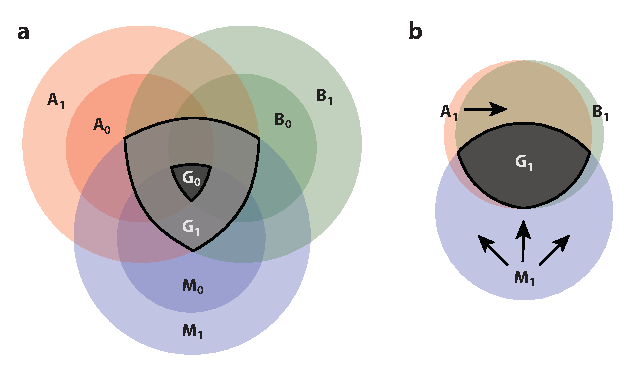
\includegraphics[width=3in]{SampleFigure}
\caption{Figure caption with descriptions of parts a and b}
\label{fig1}
\end{figure}

% Example of a Table
\subsection{Tables} Tables should also be cited in the main text in chronological order (\textbf {Table \ref{tab1}}).

\begin{table}[h]
\tabcolsep7.5pt
\caption{Table caption}
\label{tab1}
\begin{center}
\begin{tabular}{@{}l|c|c|c|c@{}}
\hline
Head 1 &&&&Head 5\\
{(}units)$^{\rm a}$ &Head 2 &Head 3 &Head 4 &{(}units)\\
\hline
Column 1 &Column 2 &Column3$^{\rm b}$ &Column4 &Column\\
Column 1 &Column 2 &Column3 &Column4 &Column\\
Column 1 &Column 2 &Column3 &Column4 &Column\\
Column 1 &Column 2 &Column3 &Column4 &Column\\
\hline
\end{tabular}
\end{center}
\begin{tabnote}
$^{\rm a}$Table footnote; $^{\rm b}$second table footnote.
\end{tabnote}
\end{table}

% Example of lists
\subsection{Lists and Extracts} Here is an example of a numbered list:
\begin{enumerate}
\item List entry number 1,
\item List entry number 2,
\item List entry number 3,\item List entry number 4, and
\item List entry number 5.
\end{enumerate}

Here is an example of a extract.
\begin{extract}
This is an example text of quote or extract.
This is an example text of quote or extract.
\end{extract}

\subsection{Sidebars and Margin Notes}
% Margin Note
\begin{marginnote}[]
\entry{Term A}{definition}
\entry{Term B}{definition}
\entry{Term C}{defintion}
\end{marginnote}

\begin{textbox}[h]\section{SIDEBARS}
Sidebar text goes here.
\subsection{Sidebar Second-Level Heading}
More text goes here.\subsubsection{Sidebar third-level heading}
Text goes here.\end{textbox}



\subsection{Equations}
% Example of a single-line equation
\begin{equation}
a = b \ {\rm ((Single\ Equation\ Numbered))}
\end{equation}
%Example of multiple-line equation
Equations can also be multiple lines as shown in Equations 2 and 3.
\begin{eqnarray}
c = 0 \ {\rm ((Multiple\  Lines, \ Numbered))}\\
ac = 0 \ {\rm ((Multiple \ Lines, \ Numbered))}
\end{eqnarray}

Define Standard Model (SM), Dark Matter (DM). There is also an "acronym" section we could use. 
Need to decide whether Dark Matter or dark matter.

Most recent reviews of DD and ID (in absence of anything better?)
\cite{DMDD_NaturePhysics}
\cite{DMID_NaturePhysics}
I prefer these ones also because they have arXivs but they are older \cite{Gaskins:2016cha}, \cite{0954-3899-43-1-013001}. There is also a VERY old AR: \cite{doi:10.1146/annurev.nucl.54.070103.181244}

History of DM: ~\cite{Bertone:2016nfn}

%Throughout this review, we will consider the relic density as a rough order-of-magnitude guide for our selection of models and results, rather than as an exact constraint. Most of the models considered that satisfy the relic density only consider a single particle. The DM sector may be much more complex than a single particle with a limited number of interaactions. Nevertheless, if these simple examples dominate over others.  

%these simple examples may emerge in the searches at the early stages of the LHC  particles  

We link the observations on DM to its particle properties.

Why WIMP miracle?

Make point that we see simple things first (why simplified models is a good assumption). 

\subsection{Observations on DM as a guide for its particle properties}
\label{sec:DMObservations}

%Mention relic

The observations mentioned above require the dark matter particle to be stable on a cosmological timescale. This has important consequences for the prediction and observation of dark matter reactions at colliders, even though collider experiments are unable to measure particles on timescales that are longer than the time it takes them to cross the detector. 

\begin{marginnote}[]
\entry{DM stability and collider searches}{DM is stable on a cosmological scale, while LHC experiments are limited to the observation of particles with a lifetime that is longer than the time needed to escape the detector (i.e. DM candidate particles could still decay into other particles outside the detector and leave a signal of missing transverse momentum).} 
\end{marginnote}

Firstly, the DM particle cannot decay. Conservation laws, such as R-parity in Supersymmetry (SUSY),
can prevent this. Another simple theoretical way to stabilize DM, as in Ref.~\cite{Batell:2010bp}, 
is the introduction of a global $Z_2$ symmetry. 
\begin{marginnote}[]
\entry{$Z_2$-parity}{symmetry under which the parity of the DM particle is odd, while the parity of SM particles is even.
It is multiplicative and conserved in the models considered. }
\end{marginnote}
According to the $Z_2$ symmetry an odd-parity DM particle cannot decay into any 
lighter even-parity SM particles and it is therefore stable. 
Additionally, DM particles will be produced in pairs from the decay of other particles
that are charged under the same gauge group as the SM.
A simplified diagram of an s-channel process at colliders
satisfying $Z_2$ symmetry is shown in panel (b) of Fig.~\ref{fig:monoX}.
If the particle mediating the SM-DM interaction is a SM particle, no additional particles beyond the DM need to be invoked, leading to the simplest DM production mode at the LHC. The only theoretically viable SM portal particles within the grounding assumptions of this review are the Z and the Higgs bosons, described in Section~\ref{sec:HZPortalModels}. 

%TODO: add sidebar figure of s-channel. 
%this will become useful when we talk about s-channel mediators. maybe also make a point
%for the t-channel mediator?

Secondly, dark matter particles are invisible to traditional collider experiments. 
However, the rest of the event is not. DM particles can be accompanied by one or more
visible particles that can recoil against the DM, leading to missing
momentum in the transverse plane. 

\begin{marginnote}[]
\entry{\pt}{transverse momentum} 
\entry{\MET}{magnitude of the missing transverse momentum} 
\end{marginnote}
%CD: CMS uses this in all its plots, but i don't find it too relevant yet
%From: https://arxiv.org/pdf/1106.5048.pdf
%The following notation is used: the vector boson momentum in the transverse plane is ?qT, and the hadronic recoil, defined as the vector sum of the transverse momenta of all particles except the vector boson (or its decay products, in the case of Z candidates), is ?uT. Momentum conservation in the transverse plane requires ?qT + ?uT = 0. The recoil is the negative of the induced ?E/T.

%I don't like how this is linking up. 

%shared context: many possible new physics searches at the LHC
%problem: can't do them all
%solution: strong theoretical motivation, as well as observability
%exposition: particular case of DM

Further assumptions are needed to predict signals of DM at colliders, such
as that there is some form of interaction between DM and SM particles. 
Couplings to SM particles need to feature in the model and be sufficiently large
to produce new particles and observe their signatures in the detectors. 
%everyone thinks of WIMPs, how strong is strong, how weak is weak? quantitative question of coupling, depends on model. in the introduction: need to talk about DM properties. Weak enough that there is no visible EM signal (no light emission or absorption). Relate those properties to what the particle physics properties need to be. Have a model in mind: s-channel mediator between DM and SM, weakness of interaction comes from particle being heavy or coupling being small. DMF models have order=1 couplings. 
Models of particle dark matter include SM couplings to satisfy
cosmological observations in the thermal freeze-out case. 
Under these assumptions, and given the lack of evidence for 
DM interacting strongly with baryonic matter or its emission or absorption of light,
these couplings need to be weak. 
%A typical DM-SM coupling satisfying relic density is of the order of XXX. %CD: isn't this too model-dependent?
The only SM particle that satisfies this requirement of being
sufficiently weakly interacting is the neutrino.
However, neutrinos cannot make up the totality of DM as they 
%are not sufficiently massive 
are relativistic particles and cannot explain the galaxy structures that formed in the universe~\cite{PlehnLecturesDM}. 
%also numbers here http://www.slac.stanford.edu/econf/C040802/papers/L002.PDF
%%CITE FENG AR, BERTONE'S BOOK
%The upper bound on the neutrino content of DM is YYY. Not sure where to find this number

Unlike previous accelerators that either yielded large datasets (e.g. B-factories) or high center-of-mass energy (e.g. Tevatron), the LHC gives unprecedented access to both rare processes and high scale processes at the same time, planning to collect 3/ab by 2035 reaching the design center-of-mass energy of 14 TeV. For this reason, it is worth speculating whether the portal particles could be observed at the LHC for the first time. Models that include one or more very massive new particles beyond the SM in addition to the DM particle are also an LHC search target, and are described in Section~\ref{sec:BSMMediatorModels}. 

Portal models and models of simple BSM mediation only try to explain the presence of particle DM. They keep the SM and the DM sectors separate, and make no claim to being a solution of other shortfalls of the SM. However, the coincidence that hierarchy problem, gauge coupling unification and DM particle nature could be solved with a single theory with observable consequences at the electroweak scale, has been one of the driving reasons to develop and consider SUSY as one of the main search targets for LHC searches. These models are discussed in Section~\ref{sec:SUSYModels}.

Finally, let us return on the concept of observability of the search target mentioned above. Even general purpose particle detectors may miss certain classes of phenomena, as the initial design choices privileged searches for the Higgs boson and for particles that generally decay promptly, as predicted by models discussed so far. However, there is tension when confronting data with SM portal models, BSM mediation models and supersymmetric models compatible with the standard freeze-out scenarios. This encourages us to look for other classes of models, especially those including particles with long lifetimes, as a way to go beyond the traditional WIMP scenario. Reactions including those particles and their connections to DM are sketched in Section~\ref{sec:LLPModels}.

%%I suggest this part goes in the introduction, as it motivates enumeration of models in chapter 2 and comparisons in chapter 4. 
The observation of a signal of visible or invisible particles at an LHC experiment that could be identified as being generated by one of the reactions described in this review cannot lead to claims that DM has been discovered. This is not a reason to discount searches for DM at the LHC, as such a signal would still be a groundbreaking discovery, regardless of its interpretation. Instead, we highlight the importance of the comparison of LHC results, where DM would be produced in the lab, with the results of complementary experiments that look for signals of DM coming from space. This comparison can only take place if the same theoretical model is used to interpret both results. This motivates the enumeration of possible models in this chapter. 

%Heading 1
\section{REACTIONS FOR INVISIBLE PARTICLE SEARCHES AT THE LHC}
\label{sec:02_Reactions}
%Throughout this review, we will consider the relic density as a rough order-of-magnitude guide for our selection of models and results, rather than as an exact constraint. Most of the models considered that satisfy the relic density only consider a single particle. The DM sector may be much more complex than a single particle with a limited number of interaactions. Nevertheless, if these simple examples dominate over others.  

%these simple examples may emerge in the searches at the early stages of the LHC  particles  

In this chapter, we will link the observations on DM to its particle properties. We then enumerate the possible reactions of DM at the LHC within certain grounding assumptions, building from simple to more complex models in terms of particle content. 

\subsection{Observations on DM as a guide for its particle properties}
\label{sec:DMObservations}

The observations mentioned in Section~\ref{sec:intro} require the dark matter particle to be stable on a cosmological timescale. This has important consequences for the prediction and observation of dark matter reactions at colliders. 

Firstly, a simple theoretical way to stabilize DM is the introduction
of a global $Z_2$ symmetry, as in Ref.~\cite{Batell:2010bp}. A realization of this
symmetry can be found in R-parity in the MSSM. %citation?
Under this symmetry, the parity of the DM particle is odd, while the parity of SM particles is even. 
$Z_2$-parity is multiplicative and conserved: this 
%is Z_2 parity a thing? I don't want to have it confused with the global SM parity
implies that an odd-parity DM particle (charge -1) cannot decay into any 
lighter even-parity SM particles (charge +1) and it is therefore stable. 
Additionally, DM particles will be produced in pairs from the decay of other particles
that are charged under the same gauge group as the SM. 

A simplified diagram of an s-channel process at colliders satisfying $Z_2$ symmetry is shown in panel (b) of Fig.~\ref{fig:monoX}.
If the particle mediating the SM-DM interaction is a SM particle, no additional particles beyond the DM need to be invoked, leading to the simplest DM production mode at the LHC. The only theoretically viable SM portal particles within the grounding assumptions of this revew are the Z and the Higgs bosons, described in Section~\ref{sec:HZPortalModels}. 

%TODO: add sidebar figure of s-channel. 
%this will become useful when we talk about s-channel mediators. maybe also make a point
%for the t-channel mediator?

Secondly, dark matter particles are invisible to detectors. 
However, the rest of the event is not: one can observe DM particles
produced in the event and escaping the detector 
due to their missing momentum in the transverse plane, if they recoil against one or 
more visible SM particles. 

%I don't like how this is linking up. 

%shared context: many possible new physics searches at the LHC
%problem: can't do them all
%solution: strong theoretical motivation, as well as observability
%exposition: particular case of DM

Collider experiments have a nearly unlimited choice of theoretically
motivated DM targets to search for. 
Theoretical arguments alone are not sufficient for a DM model to be tested at the LHC: 
couplings to SM particles need to feature in the model and be sufficiently large
to produce new particles and observe their signatures in the detectors. 

%everyone thinks of WIMPs, how strong is strong, how weak is weak? quantitative question of coupling, depends on model. in the introduction: need to talk about DM properties. Weak enough that there is no visible EM signal (no light emission or absorption). Relate those properties to what the particle physics properties need to be. Have a model in mind: s-channel mediator between DM and SM, weakness of interaction comes from particle being heavy or coupling being small. DMF models have order=1 couplings. 

Models of particle dark matter include SM couplings to satisfy cosmological observations in the freeze-out case. These couplings need to be weak enough that there is no visible signal of DM particles, as there is no evidence for DM interacting strongly with baryonic matter, nor for its emission or absorption of light. A typical DM-SM coupling satisfying relic density is of the order of XXX. %CD: isn't this too model-dependent?

The only SM particle that satisfies the requirement of being sufficiently weakly interacting is the neutrino. However, neutrinos cannot make up the totality of DM as they 
%are not sufficiently massive 
are relativistic particles and cannot explain the galaxy structures that formed in the universe~\cite{PlehnLecturesDM}. %%CITE FENG AR, BERTONE'S BOOK
%The upper bound on the neutrino content of DM is YYY. Not sure where to find this number

Unlike previous accelerators that either yielded large datasets (e.g. B-factories) or high center-of-mass energy (e.g. Tevatron), the LHC gives unprecedented access to both rare processes and high scale processes at the same time, planning to collect 3/ab by 2035 reaching the design center-of-mass energy of 14 TeV. For this reason, it is worth speculating whether the portal particles could be observed at the LHC for the first time. Models that include one or more very massive new particles beyond the SM in addition to the DM particle are also an LHC search target, and are described in Section~\ref{sec:BSMMediatorModels}. 

Portal models and models of simple BSM mediation are only motivated by the observation of DM. They keep the SM and the DM sectors separate, and make no claim to being a solution of other shortfalls of the SM. However, the coincidence that hierarchy problem, gauge coupling unification and DM particle nature could be solved with a single theory with observable consequences at the electroweak scale, has been one of the driving reasons to develop and consider SuperSymmetry (SUSY) as one of the main search targets for LHC searches. These models are discussed in Section~\ref{sec:SUSYModels}.

Finally, let us return on the concept of observability of the search target mentioned above. Even general purpose particle detectors may miss certain classes of phenomena, as the initial design choices privileged searches for the Higgs boson and for particles that generally decay promptly, as predicted by models discussed so far. However, there is tension when confronting data with portal models, BSM mediation models and supersymmetric models that are compatible with the standard freeze-out scenarios. This encourages us to look for other classes of models, especially those including particles with long lifetimes, as a way to shine the search lamppost beyond the classic WIMP scenario. Reaction including those particles and their connections to DM are sketched in Section~\ref{sec:LLPModels}

\subsection{Caveats and grounding assumptions}
\label{sec:GroundingAssumptions}

%%I suggest this part goes in the introduction, as it motivates enumeration of models in chapter 2 and comparisons in chapter 4. 
The observation of a signal of visible or invisible particles at an LHC experiment that could be identified as being generated by one of the reactions described in this chapter cannot lead to claim that DM has been discovered. This is because DM is stable on a cosmological scale, while LHC experiments are limited to the observation of particles with a lifetime that is longer than the time needed to escape the detector (i.e. DM candidate particles could still decay into other particles outside the detector and leave a signal of missing transverse energy). This is not a reason to discount searches for DM at the LHC, as such a signal would still be a groundbreaking discovery, regardless of its interpretation. This statement highlights the importance of the comparison of LHC results, where DM would be produced in the lab, with the results of complementary experiments that look for signals of DM coming from space. This comparison can only take place if the same theoretical model is used to interpret both results. This motivates the enumeration of possible models in this chapter. 

To define the scope of the reactions for invisible particles at colliders considered in this review, we make a number of grounding assumptions: 

\begin{enumerate}

\item We describe models where the DM particle interacts with SM particles, either directly or indirectly;
\item We restrict our list to models that include a $Z_2$ symmetry to stabilize DM;
\item We privilege models that respect Minimal Flavour Violation (MFV), which imposes that the flavor structure of couplings between DM and ordinary particles follows that of the SM.  %CITE?
%Citation from DMFs
%[49] J. Abdallah, H. Araujo, A. Arbey, A. Ashkenazi, A. Belyaev, et al., Simplified models for dark matter searches at the LHCSubmitted to Phys.Dark Univ. arXiv:1506.03116.
% [47] A. A. Petrov, W. Shepherd, Searching for dark matter at LHC with mono- Higgs production, Phys.Lett. B730 (2014) 178–183. arXiv:1311.1511, doi:10.1016/j.physletb.2014.01.051.
% [51] R. S. Chivukula, H. Georgi, Composite Technicolor Standard Model, Phys.Lett. B188 (1987) 99. doi:10.1016/0370-2693(87)90713-1.
% [52] L. Hall, L. Randall, Weak scale effective supersymmetry, Phys.Rev.Lett. 65 (1990) 2939–2942. doi:10.1103/PhysRevLett.65.2939.
% 2570 [53]
% A. Buras, P. Gambino, M. Gorbahn, S. Jager, L. Silvestrini, Universal unitarity triangle and physics beyond the Standard Model, Phys.Lett. B500 (2001) 161–167. arXiv:hep-ph/0007085, doi:10.1016/S0370-2693(01) 00061-2.
% 2575
% [54] G. D’Ambrosio, G. Giudice, G. Isidori, A. Strumia, Minimal Flavor Viola- tion: An effective field theory approach, Nucl.Phys. B645 (2002) 155–187. arXiv:hep-ph/0207036, doi:10.1016/S0550-3213(02)00836-2.
\item We primarily consider models where DM is a Dirac fermion, relying on existing theory material developed for early Run-2 searches. Other cases yield similar phenomenology for LHC searches, with some exceptions that we describe in this chapter. 
\item We privilege models that have a connection with thermal relic from freeze-out. We remark however that there are other models from other cosmological histories (e.g. freeze-in) that can be considered and would lead to interesting LHC signatures~\cite{Bernal:2017kxu}. 
%The Dawn of FIMP Dark Matter: A Review of Models and Constraints  - https://arxiv.org/pdf/1706.07442.pdf, Minimal Decaying Dark Matter and the LHC - https://arxiv.org/pdf/1305.6587.pdf
%
\end{enumerate}

%Caveat??
In the following sections will describe models from the perspective of experimental collider physicists, focusing on a selection of models that provide distinct and testable LHC signatures, without the ambition of theoretical completeness. For other perspectives on the models used for early LHC searches for DM, see~\cite{Kahlhoefer:2017dnp,Abercrombie:2015wmb,Arcadi:2017kky,Ellis:2010kf}. %Cite SUSY review by Feng?

\subsection{Higgs and Z boson portals}
\label{sec:HZPortalModels}

Even if we cannot observe DM itself at colliders, we can look for visible particles that are associated to Dark Matter. The LHC alone cannot solve the strong CP problem through observation of the axion, but it can still observe e.g. scalar resonances that appear in the theory. %CD: I think axion is out of place here

This raises the question of whether any of the SM particles could be associated to DM, for example in a similar fashion as the W and Z bosons mediate the weak interaction and produce neutrino pairs in the reaction. Models where the SM particle sector is coupled to the dark sector through an existing or a new particle are called \textit{portal models}. This kind of model leads to the most economical particle content for reactions at the LHC, as one only needs to add a neutral DM particle to the SM content if one of the SM particles is the portal particle. SM fermions cannot be portal particles under the assumption of a $Z_2$ symmetry, as they would allow the decay of DM. Photons, W bosons and gluons can't be portal particles either, as DM does not absorb nor emit light, nor it does it have electromagnetic or strong charge. The only viable SM portal particles remaining are the Z and the Higgs bosons. 

There are strong theoretical and experimental arguments to explore SM portal models at the LHC. 
%Theoretical
Processes involving mediators at the electroweak scale are among the first to be investigated, in DM theories that predict new weakly interacting particles~\cite{Cotta:2012nj}. This kind of portals are also present in a number of other theories~\cite{Arcadi:2014lta}. %CD: are there earlier monoZ papers?
%Experimental 
However, it is only the recent generations of collider and direct detection experiments that have started being able to probe the range of small couplings and relatively large scales required to observe this kind of models. 

\subsubsection{Z portal models}

The \textbf{Z portal} model, where the DM particle has vector and axial vector interactions with a Z boson, is a minimal extension of the SM as it only requires a single new particle to be added to the SM particle content. In $SU(2)_L \times U(1)$ extensions of the SM, the axial and vector couplings of the Z boson to DM are generally required to be of the same order. If no other couplings are present, this model is not $SU(2) \times U(1)$ invariant, unless couplings to the DM to the Higgs boson are added as well~\cite{Kahlhoefer:2015bea}. 
%The couplings between the Z and the DM can be vector, axial or mixed. 
In the minimal case where the couplings do not depend on the Lorentz structure of the interaction, 
%what I want to say: In general they are excluded in their minimal version because of their strong vectorial coupling necessary to respect relic abundance bounds.
large couplings are required for this model to satisfy the relic density. 
In the case of equal vector and axial couplings, this model is heavily constrained by LEP and direct detection experiments (see e.g. Refs.~\cite{Arcadi:2014lta,Escudero:2016gzx}). This model can still be viable wherever no relations between the vector and axial couplings are present. A review of Z portal models with different couplings can be found in Ref.~\cite{Arcadi:2014lta}. 
%Does one require a certain kind of couplings for symmetries? 
%Arcadi says: 
%In all these extensions, the axial coupling Aχ (see eq.(1)) of the Z boson to the dark matter is naturally of the order of magnitude of its vectorial coupling Vχ. The deep reason is that in a framework of SU(2)L × U(1) breaking the original SU(2)L condition (Vχ = Aχ) is only mildly modified by the dynamic of the breaking. 
%Maybe link this to the choices for the Z' model later on? 

\subsubsection{Higgs portal models}

The discovery of a SM-like Higgs boson~\cite{Aad:2012tfa,Chatrchyan:2012xdj} has sparked theoretical and experimental interest in \textbf{Higgs portal} models, where DM particles can interact with SM particles only through the Higgs boson (see e.g. Refs.~\cite{Patt:2006fw,Englert:2011yb,Djouadi:2011aa}). In Higgs portal models, DM couples to the SM operator connecting two Higgs fields and could dominate the interactions between SM and DM sectors.
%since the $H\dagger H$ operator has the lowest dimension in the SM. 
This interaction is renormalizable and leads to a UV-complete, minimal theory in the case of scalar and vector DM, while a self-consistent theory requires the presence of further particles mediating the interaction in the case of fermion DM~\cite{Freitas:2015hsa}. 

%From http://iopscience.iop.org/article/10.1088/1126-6708/2008/07/058/pdf
%Higgs-sector and Z′ interactions between the hidden sector
%and the SM states are special in that they involve gauge-invariant operators of dimension
%dO ≤ 4, and thus can be induced by physics at arbitrarily high scales with unsuppressed
%couplings. 

The properties of the Higgs boson are modified in the presence of decays to invisible particles. Precision measurements of the Higgs width and couplings offer a probe for these models complementary to direct searches for the invisible particles, as described in the next chapter. 
%This class of models is already constrained by electroweak precision measurements, but still viable if the DM mass is about half the Higgs mass. 

%We could have a picture of constraints here?

%Arcadi
%However, the last LUX results[11], combined with the invisi- ble width of the Higgs excluded the Higgs-portal scenario for dark matter mass below 200 GeV [2].

\subsection{Effective Field Theories and Simplified models of BSM mediators}
\label{sec:BSMMediatorModels}

Having completed the survey of the possible minimal DM models that only add a single new DM particle to the SM, we move to the next class of models, where the SM particle spectrum is complemented by the DM particle as well as by other BSM particles. In this case, the LHC search targets expand from the excess of missing transverse momentum to a wide variety of observable signatures from e.g. the decays of the new BSM particles. 

The huge body of theoretical literature on DM models featuring additional BSM particles drives the design of experimental searches in two complementary directions. In the case of self-consistent models of DM such as fully-developed SUSY models, all experimental handles are exploited for targeted searches that are sensitive to specific model features. These models will be described in the next section. However, the desire to make no assumptions on the DM phenomenology and to cast a net as wide as possible remains. The adoption of much simpler model as first LHC Run-2 DM benchmarks led to the design of more generic searches targeting the broad features of those models. The success of such simple, at times incomplete and not always theoretically sound models has been due to their ability to predict the key features and observables related to DM production at the LHC with only a limited number of new particles and theory parameters, factoring out the more complex processes that do not affect LHC phenomenology as they e.g. occur at higher energy scales. As proven by the history of SM discoveries, this simple approach can be used to discover the most prominent DM-SM interaction processes in the wake of the LHC start-up. 

These simple models have generally been organized according to their interactions and observable consequences~\cite{Goodman:2010ku,Abercrombie:2015wmb}, used as building blocks for more complex theories in models of DM and elsewhere, see e.g ~\cite{Alwall:2008ag, Agrawal:2010fh, Alves:2011wf, Choudhury:2015lha, Gutschow:2012pw}, and employed for building a prioritized set of LHC search scenarios that is only loosely connected to specific theories of DM. 
Even in the case of simple models, this review lays grounding assumptions on what is covered, similarly to what has been done for the first LHC searches. In addition to the grounding assumptions discussed in Section~\ref{sec:GroundingAssumptions}, we restrict to models where the leading process is tree-level, leaving cases where the dominant contributions are of higher order for later study (see e.g. Ref.~\cite{Godbole:2015gma}). 

\begin{figure}[!htpb]
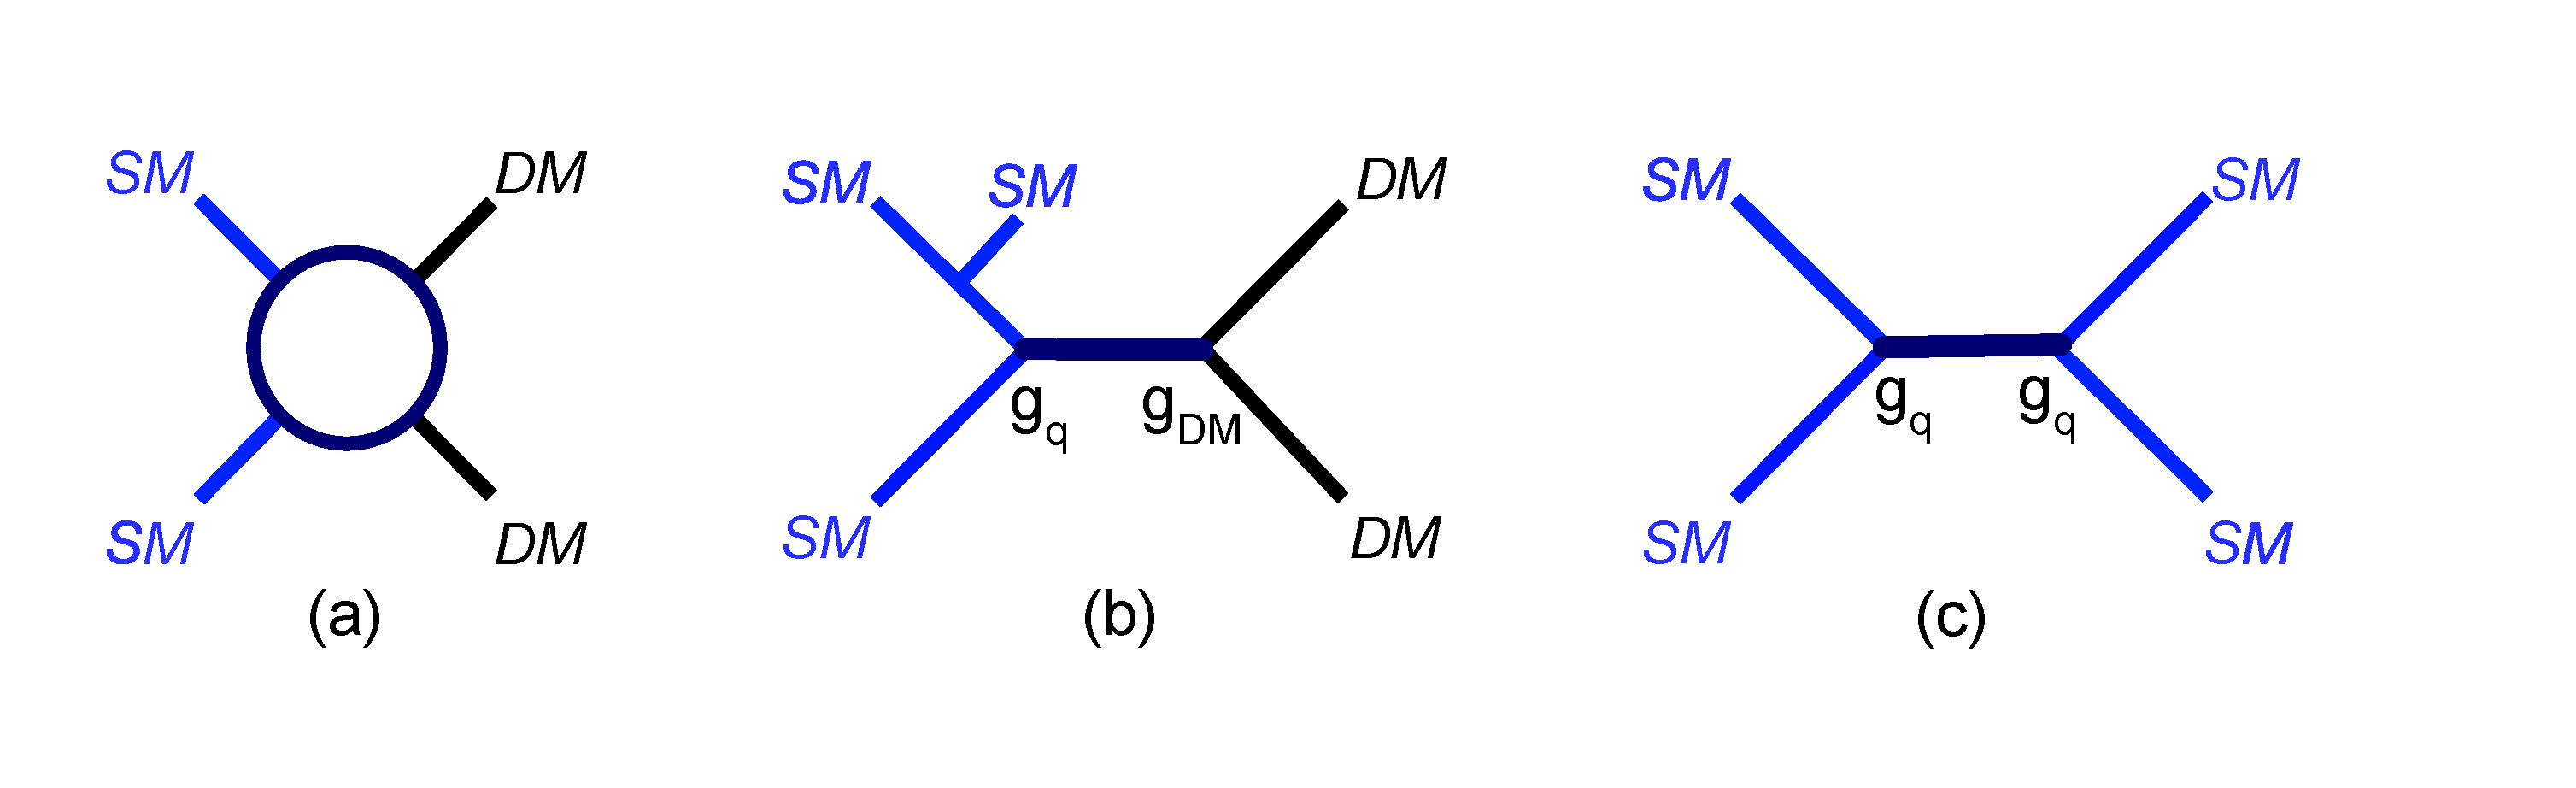
\includegraphics[width=\textwidth]{figures/MonoX.pdf}
\caption{Sketches of (a) the basic Standard Model (SM) - Dark Matter (DM) interaction at colliders in an effective field theory (EFT), (b) its extension as a basic simplified model where a new mediator particle is exchanged in the s-channel (including an additional energetic object radiated from one of the initial state quarks) and (c) the same simplified model where the mediator decays back into SM quarks. The coupling constant characterizing the mediator-quark interaction strenght is denoted as \gq, while the mediator-DM coupling constant is denoted as \gdm. From~\cite{monoXfig}.}
\label{fig:monoX}
\end{figure}

\subsubsection{Effective Field Theories}

\textbf{Effective field theories} (EFTs)~\cite{Goodman:2010ku, Shoemaker:2011vi} are the simplest possible models of DM production at the LHC beyond those described in Section~\ref{sec:HZPortalModels}. A four-point interaction is used to describe the DM production at the LHC in a low-energy approximation of a full theory, similarly to what done when describing the weak interaction through a Fermi process before the introduction of the W and Z bosons~\cite{Fermi2008}. EFT operators were first widely employed to describe DM reactions at colliders at the Tevatron~\cite{Bai:2010hh,Beltran:2010ww}. They were found advantageous because of their model-independence, and since each of the operators encapsulates the phenomenological characteristics of most known types of SM-DM interaction. A sketch of an EFT process at the LHC is shown in panel (a) of Fig.~\ref{fig:monoX}. 

The only parameter characterizing an EFT operator, in addition to the type of DM particle and to the type of SM-DM interaction, is the scale of the contact interaction $\Lambda$. In the case of a $s-$channel completion of the EFT, this interaction scale is proportional to the mass of the mediator particle. If the scale of the DM interaction is sufficiently low with respect to the mediator mass, the phenomenology is the same for the EFT as for its $s-$channel completion. 
This may not always be the case at the LHC, given the high center-of-mass energy collisions: a better description of both theory and phenomenology can be reached when explicitly including the new particles in the model considered~\cite{Buchmueller:2013dya,DeSimone:2016fbz,Berlin:2014cfa}. Certain EFT operators also may suffer from gauge invariance issues at the electroweak scale~\cite{Bell:2015sza}. However, if no completion is available, EFTs are still a good benchmark to motivate the exploration distinct kinematic regions and signatures at the LHC. %Maybe mention that obscure model we have in DMF report?

\begin{marginnote}[]
If a completion of the EFT is not available, procedures describing how to truncate the events where the EFT description is not valid are available~\cite{Racco:2015dxa,Busoni:2014sya,Busoni:2013lha,Busoni:2014haa}. A recommendation on how to present EFT results from LHC searches can be found in~\cite{Abercrombie:2015wmb}.
\end{marginnote}

Run-1 LHC searches privileged EFT operators, while Run-2 searches are limited to using EFT models with a SM singlet and a boson pair, coupled to DM through a contact interaction (see e.g.~\cite{Petrov:2013nia,Berlin:2014cfa}). [TODO CD: find completion: maybe Linda's talk at some old DMWG? AB may have more luck with trilobyte searches]


\subsubsection{Simplified models}
\label{sub:simplifiedModels}
 
%CD: this sentence does not really work
Simplified models of BSM mediation are a natural step beyond effective operators and still map well to the different types of interactions. 

Simplified models resolve the issue of whether a model-independent EFT description is valid at the LHC, even though they are not complete models themselves (e.g. not all the models used are gauge invariant~\cite{Kahlhoefer:2015bea}). Simplified models can be used for comparisons with non-collider DM searches within a clearly specified theory framework. Their use as benchmark models for Run-2 searches also highlights the strength of the LHC in searching for the visible decays of the mediator particle alongside its decays in DM particles, as detailed in the next chapter. 

For a comprehensive review of WIMP simplified models of DM at the LHC, we refer to~\cite{Arcadi:2017kky}, while~\cite{Abercrombie:2015wmb} presents a prioritized list of simplified models that have been used in early LHC Run-2 searches. The prioritized, compact set of benchmark simplified models in~\cite{Abercrombie:2015wmb}, as well as their parameters, have been discussed and agreed upon during a joint experimental and theory effort called the Dark Matter Forum (DMF), now Dark Matter Working Group within the LHC Physics Centre at CERN (LPCC)~\cite{DMWG}. 

\begin{marginnote}[]
The DMF was built starting from the discussion of various communities in Refs.~\cite{Yavin:14092893,Malik:2014ggr,Abdallah:2015ter}. All models covered in~\cite{Abercrombie:2015wmb} are available on the DMF git repository. Add reference. 
\end{marginnote}

In the simplified models chosen as benchmarks for the first LHC Run-2 searches, only one extra particle is added to the the DM and SM particle spectra. In general, this particle mediates the DM-SM interactions. If neutral, the mediator particle is singly-produced at the LHC, and decays in pairs of DM particles due to the $Z_2$ symmetry as well as in pairs of SM particles. If the mediator is colored, it can lead to a $t-$channel exchange between an incoming LHC parton and the DM particle. The phenomenology of colored mediators of DM is akin to that of SUSY models with a squark exchange~\cite{Papucci:2014iwa,An:2013xka,Bell:2012rg} with some differences that we will review later in this section. 

Early LHC searches have initially privileged $s-$channel resonances as benchmark models, as a generalization of the simplest portal models described in the previous section. Resonances decaying in two bodies
%, be those visible or invisible particles, 
are a simple, attractive benchmark to be directly produced at particle collider that has just increased its center-of-mass energy. These resonances can be classified according to their spin: spin-1 vector or axial vector mediators (also called Z'), scalar mediators (termed $\phi$ in the following) and spin-2 vector mediators. This review does not cover in detail spin-2 mediators as they have not yet been adopted as benchmark models by LHC searches, even though they produce diboson signatures that are not present in other models. More information on spin-2 mediators can be found in e.g. Refs.~\cite{Kraml:2017atm,Han:2015cty}.

%CD question: introducing parameter scans is too long. 
%CD gut feeling: it would be good to have some pictures to break this up? 
%CD TODO: mention relic for all of these? 
%CD maybe would prefer to move "when do we see this at the LHC" to the next section? 

%%%s-channel
%General
\textbf{Massive spin-1 bosons with axial or axial vector couplings} to SM and DM particles~\cite{Shoemaker:2011vi} are common in many theories, beyond those of DM mediation. They can be considered as heavy copies of the SM Z boson that arise from breaking of larger gauge groups, and as such they can be contained in larger models. A relevant characteristic of this model for LHC phenomenology is that if the Z' couples to quarks (as it needs to, in order to be produced at the LHC), then it must have visible decays back into quarks. This opens a new avenue for searches of this new particle in dijet signatures with sensitivity in early LHC data, complementing searches for excesses of missing transverse momentum. 

%Parameters
The simplest incarnation of kind of model, where the Z' only couples equally to each kind of quarks and to DM, is fully defined given the nature of the Z' couplings (vector, axial vector or mixed), their magnitude (\gq and \gDM), the mass of the DM particle \mdm and the mediator mass \mmed. The nature of the Z' couplings (vector, axial vector or mixed) does not change the LHC phenomenology, but changes the comparison of LHC results to DD and ID searches. Axial vector are the most widely used LHC benchmarks as DD rates are suppressed. [CD: specify more?]. 

%Additions: Higgs and Z' models
Vector and axial vector mediator models can include couplings of the Z' to the Higgs boson, so that the Z' boson can acquire mass through a new baryonic Higgs $h_B$~\cite{Berlin:2014cfa}. This collapses to the simpler vector model in the limit of very heavy Z' mass. When the interaction between the Z' and the SM Higgs is relevant, it can be parameterized using the Z'-SM Higgs coupling \ghZprimeZprime, the mixing angle between the SM Higgs and the baryonic Higgs, \sinthetab, the vacuum expectation value of $h_B$. This model can also lead to mono-Z signals, if the Z' is allowed to interact with the Z and the photon through kinetic mixing, but this interaction has been negleccted in LHC Run-2 searches so far. 
%CD: is there a paper by Vichi on this topic? Can't find it

%Problems
In certain region of this parameter space, especially at low mediator masses, the leptophobic Z' model can satisfy the relic density constraints~\cite{Chala:2015ama}. However, if taken in isolation, these models are  non-renormalizable, and the axial vector model violates perturbative unitarity in certain regions of the parameter space (see Ref.~\cite{Boveia:2016mrp} and references therein) if \mdm is larger than \mmed. 
%CD: and references therein = maybe we should cite original papers? 

%General, reasons for doing it at the LHC
If the mediator is a real scalar or a pseudoscalar singlet, it can have tree-level interactions with DM.
\textbf{Color-neutral scalar and pseudoscalar bosons} mediating SM-DM interactions (see e.g. Refs.~\cite{Buckley:2014fba}) take advantage of the theoretical and experimental body of knowledge that led to the recent discovery of another scalar boson, the Higgs boson. Minimal Flavor Violation dictates that the coupling of these new bosons to fermions should be proportional to those of the Higgs boson to escape flavor constraints (see Ref. ~\cite{Dolan:2014ska} for a description of remaining constraints for pseudoscalar searches), and therefore that their visible decays should be dominated by heavy-flavor quarks. Other parallels with LHC Higgs phenomenology are the importance of loop-induced couplings to gluons in the production of scalar and pseudoscalar mediators~\cite{Haisch:2015ioa,Mattelaer:2015haa} and the associated production of the mediator together with heavy flavour quarks~\cite{Buckley:2014fba}. Scalar and pseudoscalar models have much lower cross-sections than their vector and axial vector counterparts in the same fashion as the Higgs production cross-section is suppressed with respect to the Z cross-section in the SM, but the associated heavy quarks provide experimental handles that make those models testable at the Run-2 LHC. Single top signatures are also in reach of LHC searches~\cite{Pinna:2017tay}, as they are kinematically favored even though their production cross-section is generally lower with respect to the associated production of a pair of top quarks. %CD: this is interesting and new, but may be cut if we need to cut. 

%Parameters
Color-neutral scalar and pseudoscalar models are fully defined given the masses of the DM particle and of the mediator, the nature of the $\phi$-DM couplings (\gdm) and $\phi$-fermion (\gq) couplings. Following the convention in~\cite{Abercrombie:2015wmb}, \gq is a pre-factor to the Yukawa couplings of the mediator to fermions and it is considered equal for all quarks in early LHC searches. 
The LHC kinematics of models with scalar and pseudoscalar mediators assuming the same couplings is degenerate. Since the pseudoscalar model has been favoured for the interpretation of the DAMA and galactic center excess~\cite{Arina:2014yna,Agrawal:2014una} and collider searches are favored when comparing to DD~\cite{Banerjee:2017wxi}, LHC searches have privileged this choice and considered the associated scalar boson as decoupled at higher energies. 

%Additions: Higgs models
\begin{marginnote}[]
\vskip-100pt
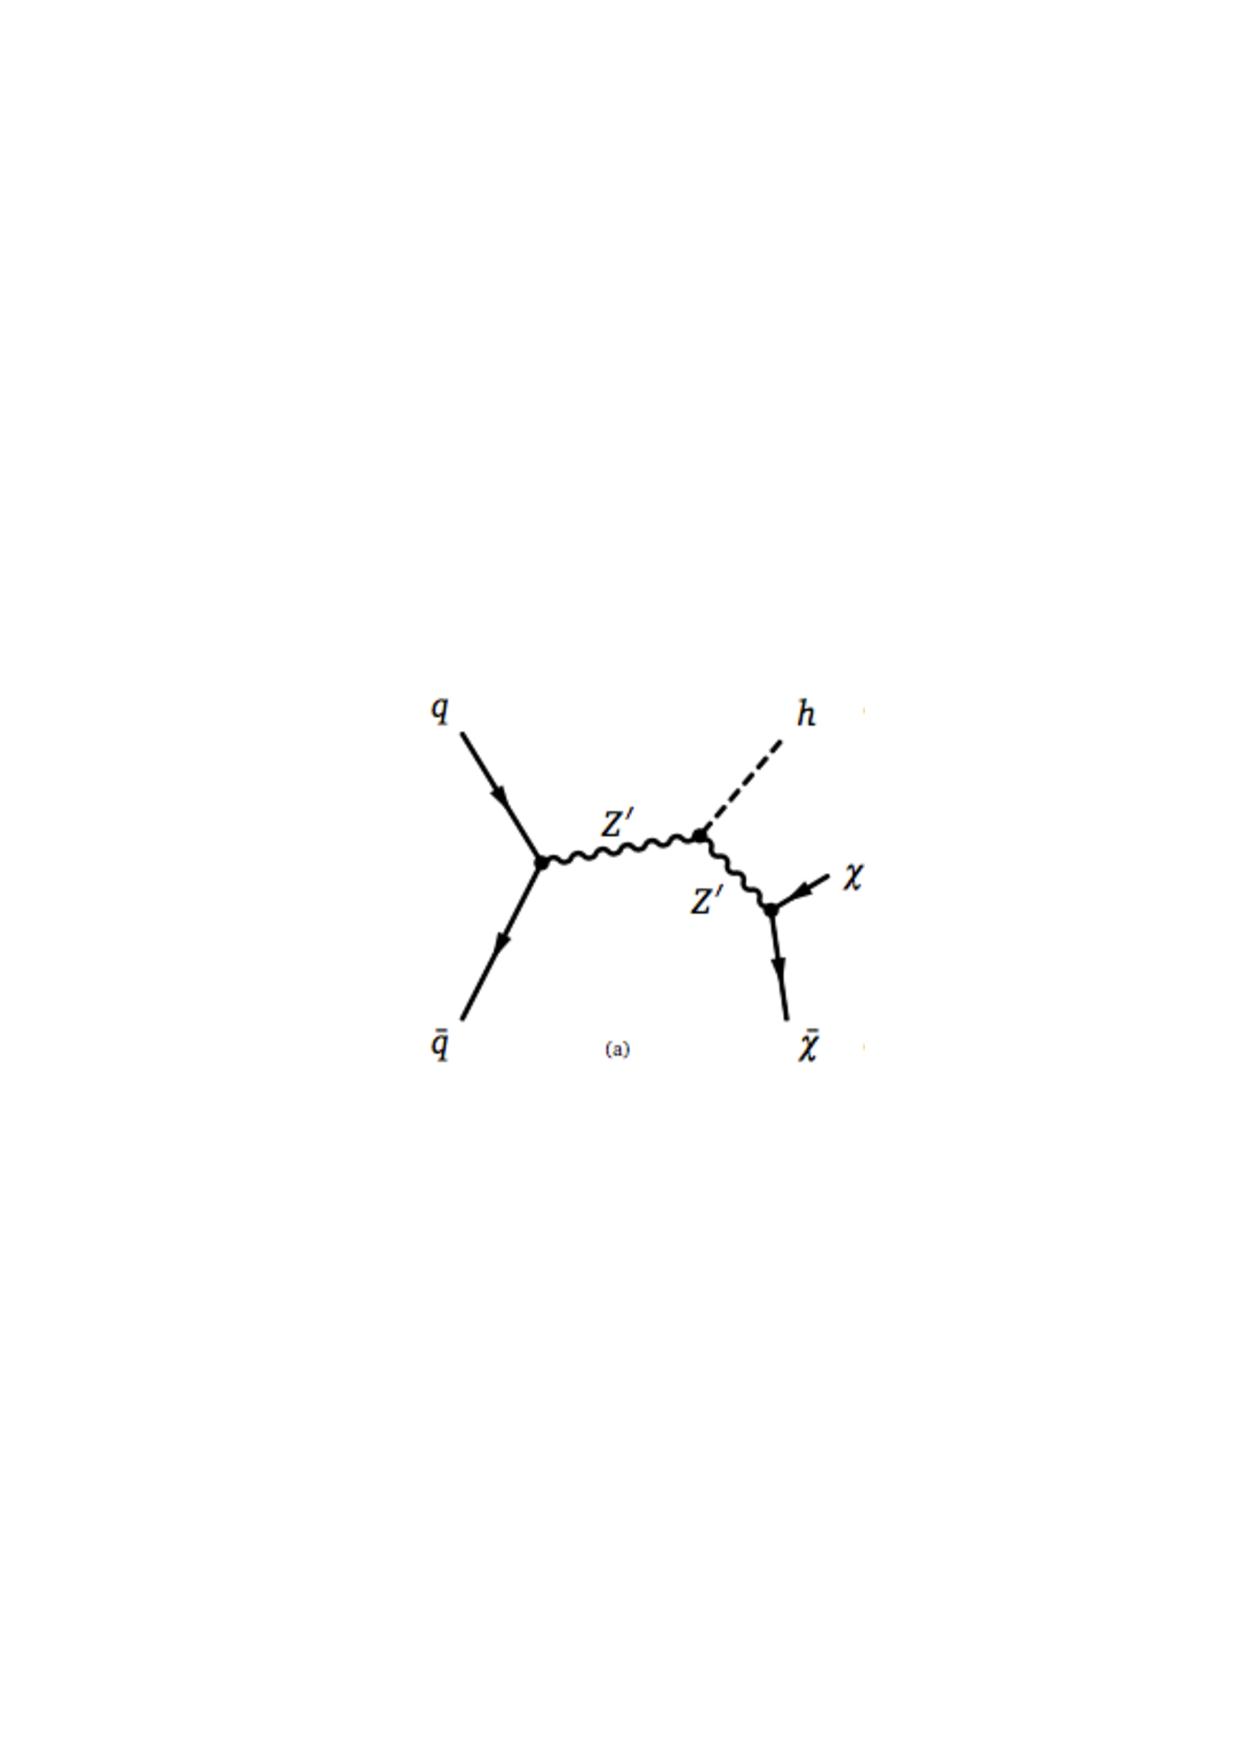
\includegraphics[width=0.5\textwidth]{figures/test-feynman.pdf}
\vskip-100pt
Feynman diagram testing things. We could do this and it's informative, but positioning will be a pain. 
\end{marginnote}

%CD: this needs a feynman diagram otherwise one gets confused
In the most general scalar potential, the scalar can couple to DM through a Higgs portal~\cite{Berlin:2014cfa}. The scalar mediator mixes with the SM Higgs boson with a mixing angle \sinthetahS and with a new physics coupling $b$ that can be set to unity, and to DM through a Yukawa term as above. This model adds mono-Higgs signals to the signatures of the scalar model without Higgs couplings. The mixing angle is constrained from current Higgs precision measurements to be \sinthetahS $<$ 0.4, and the LHC kinematics does not depend on this mixing angle. Couplings to other MS particles, notably EW gauge bosons, can also be added as a consequence of electroweak symmetry breaking as in ~\cite{Bauer:2016gys,Englert:2016joy}. The signatures of this latter model include invisible decays of the Higgs boson if the DM particle is lighter than the SM Higgs, as well as signals of Higgs and vector bosons plus missing transverse momentum at tree level. 

%CD: check back on emails with DiFranzo

%Problems
If the mediators are pure SM singlets, the model is not invariant under $SU(2)_L$~\cite{Bell:2016ekl}. 
%Maybe add Uli/No/etc's papers here?
To restore gauge invariance, the mediator needs to mix with the Higgs sector, introducing further complexity of interactions. However, as we will see in Sec.~\ref{sec:LessSimplifiedModels}, this complexity does not translate into significant changes in the LHC kinematics of the simplest models, but rather adds extra signatures for LHC searches.

%%%t-channel, colored
%General
\textbf{Scalar and pseudoscalar bosons that possess a $Z_2$ charge} take simplified models used at the LHC beyond $s-$channel SM-DM interactions~\cite{Bai:2013iqa, Papucci:2014iwa, An:2013xka, Bell:2012rg} as they mediate the interaction between a DM particle and a SM quark. Models including color triplets of this kind have historically been called $t-channel$ models, but their diagrams are not exclusively of simple $t-$channel mediation. In these particular diagrams, a scalar that is colored under SU(3) is exchanged, analogously to a squark exchange in the MSSM where only squarks and neutralino are light.
With respect to the $s-$channel mediator models, models with a colored scalar mediator have a broader set of multi-jet signatures and kinematic features that make it interesting in terms of LHC phenomenology~\cite{Abercrombie:2015wmb}. %This will be substituted by the DMWG write-up if it comes in time. 
Another handle for LHC searches is the radiation of a Z boson by the right- and left-handed mediators, as well as a W boson by the left-handed mediator~\cite{Bell:2012rg}. 

%Parameters
The definition of the parameter space for colored mediator models requires setting the mass of the mediators and of the DM particle. The mediator mass is set equal for all mediators due to the MFV assumption, and the mediator must be heavier than the DM particle to ensure DM stability. 
%Requirement of the width: mChi^2+mq^2<=Mmed^2
The coupling between DM and quarks \gdmq in LHC searches have been set to be universal but only to the first two quark generations, violating MFV. 
%CD: the following sentence does not have a source, and the Bell model only uses left-handed quarks. This is a question for Millie and the theorists present tomorrow. 
However, if only right-handed, down-type quarks are considered, flavour constraints still do not exclude a significant part of the parameter space~\cite{Abercrombie:2015wmb}. 

As opposed to the MSSM, the coupling between DM and quarks in this simplified model is not a priori fixed or constrained by the necessity of fitting within a more complex, self-consistent particle spectrum. The couplings required for this model to satisfy the relic density are generally higher than what used by SUSY models. 
%Citation to MG's studies?
Couplings to vector bosons also allow the mediator to radiate a W or a Z, leading to LHC signatures that can be targeted by specific searches~\cite{Bell:2012rg}. 
%Problems 
More sophisticated models that satisfy the full SM gauge symmetry and MFV include third generation couplings and lead to two independent mediators and couplings are described in Ref.~\cite{Ko:2016zxg}. 
The parameters and couplings of this model have also been tuned to explain the gamma ray excess and motivate searches with a single $b-$quark in the final state~\cite{Agrawal:2014una}, leading to a similar phenomenology as the MSSM with a light bottom squark and neutralino. 
%Top-flavored models also exist in literature but have not been used as benchmarks in LHC searches. 

\subsubsection{Consequences of $s-$channel mediated models: visible decays}
\label{sec:MediatorSearches}

As mentioned in the earlier section, if the mediator particle is produced from from interactions of
quarks and gluons, it will also decay in quarks and gluons. 
For this reason, it is worthwhile that collider experiments not only search for
the invisible Dark Matter particles, but also probe directly the interaction between Standard Model and 
Dark Matter particles by searching for the visible decays of the particles that mediate it, as shown 
in Figure~\ref{fig:monoX} (c) and summarized in e.g. Refs.~\cite{Liew:2016oon,Fairbairn:2016iuf}. 

%CD cite the following
%Coupling--mass mapping of di-jet peak searches, 10.1103/PhysRevD.88.035021 ok
%Searches for Dijet Resonances at Hadron Colliders, 10.1142/S0217751X11054905 in the experimental part, i would say
%Searching for Low Mass Dark Portal at the LHC, 10.1016/j.dark.2013.03.002 ok
%Constraining Dark Sectors with Monojets and Dijets, 10.1007/JHEP07(2015)089 ok
%Constraints on Z? models from LHC dijet searches and implications for dark matter - https://arxiv.org/pdf/1605.07940.pdf -> ok

Dijet searches are sensitive to vector and axial vector DM mediators decaying 
exclusively to jets with couplings that would satisfy relic density constraints~\cite{Chala:2015ama},
but also to new, unknown particles that might be created when crossing 
the threshold of a new energy scale. For the same reason, 
it is not possible to claim a discovery of DM mediators at the LHC without
corresponding excesses in invisible channels and non-collider experiments. 
Nevertheless, these benchmark models have motivated novel search techniques
to look for low-coupling, low-mass resonances below the TeV scale that would
have otherwise not been explored in early Run-2 data due to experimental difficulties~\cite{An:2012ue,Dobrescu:2013coa}. 

The leptophobic vector and axial vector simplified models described in \ref{sub:simplifiedModels} 
are however not always theoretically viable, as lepton decays are needed for gauge invariance
or are included through radiative corrections leading to a mixing between the Z' and the Z 
(see Ref.~\cite{Albert:2017onk} and references therein). A simple extension of the leptophobic vector
and axial vector models allows the mediator to decay into leptons at tree level. 
As explained in the next sections, dilepton resonances are often more sensitive than dijet resonances
at the LHC. Decays of the spin-1 mediator into neutrinos are also required by gauge invariance, and add 
an invisible decay channel that can enhance signatures of missing transverse momentum, depending on
the size of the couplings~\cite{Albert:2017onk}. 

%All citations from DMF, probably want to save citations for later
%They are sometimes necessary in order to construct a consistent theory, for example in minimal completions of the axial-vector model [11, 12] or in models with extended Higgs sectors [13, 14]. They often appear in anomaly-free spin-1 mediator models [15], see also Section 3.3.2 of [7]. They may also be induced through radiative corrections (e.g. through quark loops that lead to Z??Z mixing). The near-ubiquity of lepton couplings in full theories motivates including them when searching for visibly-decaying spin-1 mediators.

%Generic resonance searches sensitive to a broad range of theoretical models 
%are already the focus of LHC. 

\subsubsection{Less simplified models}
\label{sec:LessSimplifiedModels}

The initial list of models recommended to the experimental collaboration by the Dark Matter Forum described above is a first set of simple, mostly tree-level processes targeting early Run-2 searches. Targeting one simplified model at a time however does not cover the full complexity of LHC signatures and kinematic distributions in more complete models. Exclusively considering simplified models therefore presents the risk of missing important search targets. Moreover, UV-complete models are important and interesting as they offer solutions to SM problems beyond DM, as in the case of SUSY that will be discussed in the following section. 

There are a large number of these "less-simplified" models in literature, and very few of them have been explored directly by LHC searches considering them as benchmarks. In this review we will only sketch the main characteristic of a small selection of models within our grounding assumptions. This selection has different kinematic consequences and different signatures with respect to the simplified models used by Run-2 LHC searches so far. 

\textbf{Co-annihilation} models add one extra particle to the dark sector, generally close in mass to the DM particle. Examples can be found in Refs.~\cite{Buschmann:2016hkc,Baker:2015qna,Khoze:2017ixx}. The strong interaction between these two DM states drives the cosmological history~\cite{PlehnLecturesDM}, as processes involving both DM particles can efficiently annihilate DM into SM particles. In terms of LHC phenomenology, coannihilation models produce signatures of missing transverse energy and multiple hadronic jets accompanied by multiple resonant or non-resonant hadronic jets, in some cases untested by current searches~\cite{Buschmann:2016hkc}. In other cases, the small mass splitting between the two particles forces the decay of the next-to-lightest particle into the lightest particle to be kinematically suppressed, in turn leading to a sizable lifetime for the next-to-lightest particle~\cite{Khoze:2017ixx}. The late decays of the coannihilation partner give an additional experimental handle that can be used for LHC searches, as described in the next chapter.  
%Dark terminator needs Majorana particle, not mentioned although the idea of vector + scalar is interesting beyond LianTao's 2HDM
%Other~\textbf{models with two mediators, a scalar and a vector} with small couplings to SM particles have been developed to escape existing LHC constraints~\cite{Duerr:2016tmh}. 

%OOutline said monotop, but I don't know where to fit those because they don't necessarily have much to do with anything we talked so far? i would be happier to talk about monotop searches in terms of Priscilla/Deborah's studies. 

%OOutline said gluphilic, but we cited it above and we need to save space

The \textbf{evolution of scalar models} has also attracted the attention of both theory and experimental LHC community. The simplified scalar and pseudoscalar models described in Sec.~\ref{sub:simplifiedModels} are not self-consistent, if considered as stand-alone models they only focus on one experimental signature at a time. They are not considered the best benchmark model to make the most of %CD: bleurgh
the search opportunity offered by a machine that is sensitive to scalar particles with couplings of the order of those of the Higgs boson.
The first step towards more consistent scalar and pseudoscalar models is the addition of Higgs couplings and coupling to vector bosons that naturally stem from gauge invariance, as described above and in~\cite{Bauer:2016gys,Berlin:2014cfa}. A further refinement is to embed the scalar/pseudoscalar model in a more complete theory, namely a Two-Higgs Doublet Model (2HDM)~\cite{Bauer:2017ota,Ipek:2014gua,No:2015xqa,Goncalves:2016iyg,Bell:2016ekl}. 
%%Overkill?
%[1] M. Bauer, U. Haisch, F. Kahlhoefer, CERN-TH-2017-011, DESY-17-010 [arxiv:1701.07427 [hep-ph]].
%[2] S. Ipek, D. McKeen and A. E. Nelson, Phys. Rev. D 90, no. 5, 055021 (2014) [arXiv:1404.3716 [hep-ph]].
%[3] J. M. No, Phys. Rev. D 93, no. 3, 031701 (2016) [arXiv:1509.01110 [hep-ph]].
%[4] D. Goncalves, P. A. N. Machado and J. M. No, arXiv:1611.04593 [hep-ph].
%[5] N. F. Bell, G. Busoni and I. W. Sanderson, arXiv:1612.03475 [hep-ph].
In these models, the new scalar or pseudoscalar mediator mixes with the Higgs partners rather than with the SM Higgs, so that the model is still compatible with Higgs measurements. 2HDM+scalar/pseudoscalar have an interesting phenomenology that is not dominated by jet+missing transverse momentum searches but rather by the results of searches of Higgs or EW bosons+MET. A richer span of experimental signatures permits to expose uncovered regions in the parameter space of the model, as well as to highlight the complementarity between final states. 2HDM models developed for LHC searches focus on a Yukawa structure of Type-II, where the couplings are the same as the MSSM. The particle content of this model includes two CP-even bosons (one of which is the SM Higgs boson), two CP-odd bosons (of which one is the pseudoscalar DM mediator, privileged because it escapes DD constraints), two charged Higgs boson and the DM particle. Masses and couplings of these models are chosen to respect vacuum stability~\cite{No:2015xqa}, electroweak and flavour constraints, as well as to highlight the complementarity of the various experimental signatures. Depending on the parameter chosen, this model can satisfy the relic DM density, in general with values of \mdm above 100 GeV.   

%Sam's LianTao's 2HDM checks
%https://docs.google.com/presentation/d/10R9XJaoMDEhXKhd_Wx9yMXEaPl4uXR8IcmuTeLancvg/edit#slide=id.g217998804d_0_47

\subsection{Supersymmetric models and other theories}
\label{sec:SUSYModels}

[left for AB, see ooutline]

Other BSM theories including DM particle candidates that are not covered in this review are extra dimensions~\cite{Hooper:2007qk}, and DM as sterile neutrino~\cite{Adhikari:2016bei}. For AB who has book: See Bertone's book for non-SUSY candidates at the EW scale. 

\subsection{Long-lived particle models}
\label{sec:LLPModels}

%CD: this is very clumsy but in the spirit of blurting everything out, here it is

As discussed in the introduction to this chapter, the LHC does not directly detect DM, but rather uses visible objects to signal the presence of non-interacting, long-lived particles that escape detection. If the particle does not decay, then it is a good DM candidate. In many non-WIMP, dark sector models, one can postulate the existence of DM particles as well as other particles with lifetimes not long enough to be cosmologically stable. Those particles would escape conventional detection by collider experiments, as they e.g. decay half-way through the detector, and still lead to signatures of missing transverse momentum. 
However, these dark sector particles usually do not carry sufficient energy to be observed in this way, so experiments must devise methods targeting those non-standard decays. These will be discussed in Chapter FUTURE.

%taken some examples from: https://indico.cern.ch/event/606421/contributions/2558018/attachments/1445296/2226369/long_lived_overview.pdf
The main mechanisms for a partner particle to acquire a long lifetime are related to the suppression of its tree-level decays when:
\begin{itemize}
\item the partner particle has a large mass compared to its parents and decay products, so the decay proceeds off-shell, as in the case of e.g. the W-mediated pion decay in the SM;
\item the partner particle can decay to the DM particle but won't do so frequently due to the small mass splitting, as in the case of coannihilation;
\item when the couplings between the partner particle and either SM or DM particles are small, as in the case  of the Cabibbo-suppressed b-meson decays in the SM. 
\end{itemize}

In this review, we only sketch two examples of the third case, as it connects directly with the simplified models described in Sec.~\ref{sub:simplifiedModels}. If the only connection between the DM and SM is the new mediator particle, and DM can annihilate directly to BSM mediators and not viceversa (as \mdm $>$ \mmed), then the couplings of the mediator to the SM can be arbitrarily small. This happen for example when introducing a U(1)' symmetry mediated by a vector boson (a "dark boson"), leading to coupling $\epsilon$ through kinetic mixing, or when adding a scalar boson (a "dark Higgs") that only couples to the SM via a Higgs portal or via mixing with a heavy pseudoscalar in 2HDMs with a coupling $k$. 
%The latter model is interesting because ID is suppressed, but it's called the nightmare scenario.
In both these cases, the mediator (a "dark boson") can be long-lived~\cite{Pospelov:2007mp}, and its visible decays into SM particles or associated production with a SM boson provide the main collider handle~\cite{Curtin:2014cca}. 
%Z width, contact interactions
There is a large possible dark boson mass range that is still compatible with thermal freeze-out, from 1.5 GeV to 40 TeV~\cite{Das:2010ts}, and it can be probed by complementary experiments including present and future colliders. Another mechanism for generating the relic density that is compatible with very weak SM  interactions such as those of dark photons is the freeze-in scenario (see e.g.~\cite{Co:2015pka,Bernal:2017kxu}), where DM is produced from the thermal bath but never reaches equilibrium. CD: I don't understand this yet. 

Another bottom-up approach adopted in~\cite{Buchmueller:2017uqu} is to impose masses and couplings for the models described in~\ref{sub:simplifiedModels} so that they include a long-lived particle. The categorization of the models by production operator and final state permits a more systematic set of benchmarks for this kind of signatures. These models can then be mapped onto more complete theories. No attempts have yet been made however to connect these models to cosmological history. 


\section{EXPERIMENTAL RESULTS}
\label{sec:03_ExperimentalResults}
Now that we have a handle on the reactions of DM observable at collider experiments, we turn to a description of the searches and experimental constraints for DM at colliders, privileging LHC searches as they generally set the most stringent constraints. For a detailed description of the LHC and the ATLAS, CMS and LHCb experiments, we refer to~\cite{LHC2008,ATLAS2008,CMS2008}. %CD: blurb more? I'd say no. 
The first period of LHC running (2010-2012) at 7 and 8 TeV center-of-mass energy ($\sqrt{s}$) is termed Run-1, while the second period (2015-2018) is called Run-2. 
The categorization of these searches follows loosely the description of the benchmark models. We start describing searches for DM interacting through SM bosons~\ref{sec:results_ZHSearches}, then move to generic searches for signals with missing transverse momentum~\ref{sec:results_monoXSearches}, and outline the searches for complete models with DM candidates in Section~\ref{sec:results_SUSYSearches}. Throughout this chapter
%and in Section~\ref{sec:experimentalChallenges} %CD: removed in favour of sidebars
we will highlight the experimental challenges and the novel experimental techniques used to overcome them,
motivated by the strong interest in dark matter searches. 
We then conclude with searches for long-lived particles within models of DM in
Section~\ref{sec:results_LLPSearches}. %CD: need to rewrite this sentence, but the idea is: if we hadn't had DM as a motivation motivation we wouldn't have done this difficult stuff. 

\subsection{Searches for DM in interactions mediated by SM-boson}
\label{sec:results_ZHSearches}

The invisible decays of the Z and Higgs boson are the main direct targets of searches for SM-boson-mediated interactions between SM and DM particles, if the DM particle is lighter than half the mass of the boson. Above this region, Direct Detection experiments are generally more sensitive than collider experiments. 
%CD: do we need to answer "what if not"? No one seems to care, but one could maybe think of using monojet off-shell (tiny tiny region) and precision constraints for the off-shell region too, a la dijet. Main point for the moment: DD covers this region so we don't have to. 
In the SM, the Z boson can decay to a neutrino-antineutrino pair, while the Higgs boson decays into a pair of Z bosons each decaying to neutrinos. Additional decays of the Z and Higgs boson to particles beyond the SM modify the properties of the vector boson, such as width and couplings. 

%MonoZ

%CD only mentioning below because it's like a monophoton
%Simple (but somehow messy) explanation in https://cds.cern.ch/record/1750933/files/CERN-THESIS-2013-330.pdf, Hugo's student
%Hugo did it, unpublished: https://www-cdf.fnal.gov/physics/ewk/2007/ZnunuWidth/
%CDF direct: 466 pm 42
\textbf{Decays of the Z boson into invisible particles} can be constrained using the invisible Z width. It can be measured directly in Z decays in association with a photon emitted as initial state radiation. Events are selected containing a single photon, missing transverse momentum and no other sizable event activity. This selection is also used for identifying events from possible DM reactions at colliders.
%LEP combined: 503 $\pm$ 16 MeV
The total Z width has been measured indirectly at LEP~\cite{ALEPH:2005ab} leading to a measurement of the number of light neutrino families compatible with cosmology; if the partial widths of the decays into visible particles are subtracted from the total width, the invisible width can be measured to 499.1 $\pm$ 1.5 MeV~\cite{Patrignani:2016xqp}. 
%The precision of the indirect measurement is better than that of the direct measurement, due to the higher statistics and the relative ease of selection and background subtraction for the visible Z decays. %CD: omitted, no space
%The main systematic uncertainty in this case comes from the theoretical uncertainties in the simulation. CD: Carena seems to think it is an uncertainty on fast simulation
New physics effects modify direct and/or indirect Z width~\cite{Carena:2003aj}.
\begin{marginnote}[]
Direct and indirect Z width measurements must agree if the decay of the Z to a pair of invisible new particles is to be the main mechanism responsible for the deviation from the SM values. 
\end{marginnote}%CD: I think this is important to mention in the same sense as the caveats on the s-channel resonances, but it can be omitted
%in this case, an analysis of the mass of the system recoiling against the photon would provide a handle to distinguish between different BSM processes. %CD: omitted because this is possibly too handwavy but how can we summarize 4 pages of Carena in a sentence?
%Carena quantitative: At present, measurements at LEP and CHARM II are capable of constraining the left-handed Z\nu\nu-coupling, 0.45 <~ g_L <~ 0.5,  while the right-handed one is only mildly bounded, |g_R| <= 0.2.
The LEP precision measurements~\footnote{Bounds on Z to invisible decays obtained from LHC searches are not yet competitive~\cite{deSimone:2014pda}.}, as well as direct detection experiments, rule out the majority of the Z-mediated DM scenarios~\cite{Arcadi:2014lta,Escudero:2016gzx}. The LEP invisible width is well below the width one would expect if vector and axial vector models of DM were realized, for all couplings satisfying the relic density with a DM mass below 25 GeV. Direct detection experiments such as Xenon1T~\cite{Aprile:2017iyp} 
%CD: take figure 2 of Escudero:2016gzx and compare with the results of Aprile:2017iyp
rule out most of the other simplified model scenarios compatible with freeze-out relic density up to multi-TeV DM masses. 
%DM mass above 6 TeV for the vector couplings, while for axial the plot is truncated. 

%%MonoH

\textbf{Invisible decays of the H boson} within the SM only contribute to less than 0.1\% of the total decay width. For this reason, an observation of even a small contribution to the Higgs width from invisible particles would signal the presence of new physics phenomena that could be linked to DM if 2\mdm $< m_H$~\footnote{For the case of heavier DM particles, see Ref.~\cite{Djouadi:2011aa}.}. 

Pre-LHC constraints on the invisible Higgs width are derived from measurements of the ZH production channel at LEP in searches for new neutral Higgs-like bosons, where only the visible decays of the Z are observed. This is a common procedure to select events in LHC DM searches. %CD: need a number! 
It is not feasible to directly or indirectly measure the total and partial Higgs widths at a hadron collider and then extract the invisible contribution as done for the Z at LEP, as some of the decays (e.g. gluons and lighter quarks) have too large a background to be measured, the experimental resolution even for leptonic decays is large compared to the intrinsic Higgs SM width, and the kinematics of the ZH process is not fully determined as in lepton colliders. %CD: this is ambiguous also because I am not sure I fully understand the first and third points completely - need AB's help, page 2 of Dobrescu/Lykken. 
%Lykken/Dobrescu, 1210.3342: Total theoretical SM width/mass for H125: 3.2 * 10^-5 MeV, due to small Yukawa of b quark and suppression of WW*. From rates and couplings,  can extract upper and lower limits on the exotic Higgs branching fractions, which come from the upper/lower limit on the total width. This paper ignores exp uncertainties. 
%Wagner Dark Side of the Higgs boson: omit because we don't care about non-SM Higgses
%The width can be extracted from the lineshape in the low-background channel $Z \rightarrow ZZ \rightarrow 4l$, assuming a SM width. This is what CMS has done. 
%If one does not want to assume the SM width, one can still extract the width
%above 190 GeV where the experimental resolution is better. 
%what we want to see is a larger total width with less normalization because of the invisible decays
Instead, searches at the LHC either attempt to directly observe the invisible decays of the Higgs boson, or compare measurements with precise theoretical calculations of SM parameters, to reveal
%unearth? there are no worms in this article so we should change this word
discrepancies signaling new physics or indirectly place constraints on new physics phenomena. 
Higgs to invisible LHC searches using Run-1 and Run-2 data~\cite{Khachatryan:2016whc,Aad:2015pla} employ and combine the $qq \rightarrow H qq$, $qq \rightarrow VH$, $gg \rightarrow HZ$, $gg \rightarrow Hg$ Higgs production modes. 
%CD: This section is just CMS for now. Need to add ATLAS, but also cut as we're using too much space for this:
%https://atlas.web.cern.ch/Atlas/GROUPS/PHYSICS/PAPERS/HIGG-2015-03/fig_09.png
In all cases, in addition to a requirement of sizable missing transverse momentum, auxiliary visible objects are used to select the events. 
%Loop-induced signals are important. 
%For more info on importance and calculation of loops: 1605.08039, but we run out of citations and space
The events are divided in exclusive categories targeting specific production modes. The associated boson (VH) searches target the decays of Z bosons to electrons, muons light or heavy flavour quarks, while the W bosons can decay into light-flavour jets. 
The $qq \rightarrow H qq$ production mode is dominated by Vector Boson Fusion (VBF) processes, where the Higgs boson is produced in association with two hadronic jets that have a large pseudorapidity ($\eta$)
%CD: assume eta?
separation in the detector, and a large invariant mass. This topology is used to select events and discriminate between signal and background. 
%The large QCD backgrounds are suppressed by requiring that the missing transverse momentum recoils against the jets in the event. 
%If the missing transverse momentum was in the direction of the jets, there would be a chance of it coming from mismeasured jets. %CD: hmmm written this in a rush
The jet+MET search, described in more detail in the next section, is reinterpreted for the $gg \rightarrow Hg$ mode. 

%The upper limit on the invisible BR from Higgs decays is 25%. 
%ATLAS Abstract
%Direct searches for invisible Higgs boson decays in the vector-boson fusion and associated production of a Higgs boson with W/Z (Z ? ??, W/Z ? jj) modes are statistically combined to set an upper limit on the Higgs boson invisible branching ratio of 0.25. The use of the measured visible decay rates in a more general coupling fit improves the upper limit to 0.23, constraining a Higgs portal model of dark matter.
%%Precision
Precision measurements of the Higgs boson properties and the comparison with SM theory also play a role in constraining the possible contributions to new physics, as decays into invisible particles would reduce the SM Higgs production and decay coupling strengths~\cite{Khachatryan:2016vau,Englert:2011yb,Aad:2015pla}. 
%For the Higgs boson, the upper limit on the branching fraction to visible and/or invisible non-SM particles only using precision measurements is 34\%
%In case we want to say what limits these
%The main limitation for the measurement of the invisible width of the Higgs at the LHC is due to QCD uncertainties the Higgs production cross-section, which limits the sensitivity of these searches to roughly 10\% of the SM value. 

The most stringent observed upper limit on the fraction of invisible decays of the Higgs boson, combining direct and precision measurements is 23\%.
%What does it mean for Higgs portal models: DD is always better
In the case of light fermion DM with scalar couplings to the Higgs, direct detection experiment rule out most of the parameter space where the model can provide the measured relic density~\cite{Escudero:2016gzx,Djouadi:2011aa}. Due to the suppression of the cross-section for DD in the pseudoscalar case, the model is still not constrained around a small region for DM masses corresponding to half the Higgs mass and above. %CD: maybe we have to say why this is the case - essentially rates are too small, see paper by Plehn. 

\subsection{Generic searches for DM with missing transverse momentum}
\label{sec:results_monoXSearches}

%Sidebar (50 words minimum, 200 words maximum) briefly discussing a fascinating adjacent topic; insert below Literature Cited section, but indicate near which section in text the sidebar should be typeset
\begin{textbox}[!h]
\section{Details of \MET reconstruction and fake \MET rejection}
This is why this is important, this is 10 words. 
This is why this is important, this is 10 words. 
This is why this is important, this is 10 words. 
This is why this is important, this is 10 words. 
This is why this is important, this is 10 words. 
This is why this is important, this is 10 words. 
This is why this is important, this is 10 words. 
This is why this is important, this is 10 words. 
This is why this is important, this is 10 words. 
This is why this is important, this is 10 words. 
This is why this is important, this is 10 words. 
This is why this is important, this is 10 words. 
This is why this is important, this is 10 words. 
This is why this is important, this is 10 words. 
This is why this is important, this is 10 words. 
This is why this is important, this is 10 words. 
This is why this is important, this is 10 words. 
This is why this is important, this is 10 words. 
This is why this is important, this is 10 words. 
This is why this is important, this is 10 words. 
This is why this is important, this is 10 words. 
This is why this is important, this is 10 words. 

%\subsubsection{Missing transverse momentum}
%\label{sub:MET} 

%Main points:
%\begin{itemize}
%\item The measurement of \MET relies on the precise measurement of all reconstructed physics objects. 
%\item Some description of \MET significance may be needed, but it may also be too academic. 
%\item Fake \MET is rejected using quality cuts.  
%\item Pile-up needs specific techniques because of the soft terms. 
%\item \MET at the trigger level is the driving reason why we can't go lower, see next section.
%\end{itemize}

%from ooutline

%- Mismeasured MET (combining instrumental effects and beam/cosmics background)				
%	- CDF				
%		- beam background: exploit track pointing to jet and calorimeter layers				
%		- QCD: shitty method from Mario (extrapolation changing the veto)				
%	- LHC:				
%		- beam backgrounds: like CDF, more refined				
%			- can have a % of how many events would have been				
%		- QCD: matrix method a la SUSY				
%	- Other backgrounds (diboson, top)				
%		- Small so using MC				
%		- LHC has validation regions				
%			- check ttbar				

%Valerio's talk for relevant plots 
%https://indico.cern.ch/event/466934/contributions/2590281/attachments/1489278/2314178/20170706_EPS_DMatATLAS.pdf

%MET significance: in VBF CMS search
%For the 8 TeV dataset, an additional requirement is set on an approximate missing transverse energy significance variable S(Emiss) defined as the ratio of Emiss to the square root of the scalar sum of the transverse energy of all PF objects in the event [62]. Selected events are required to satisfy S(Emiss) > 4?GeV.


\end{textbox}

WIMP DM particles at colliders escape detection, and their observation requires one or more visible objects in the same event. Searches that only rely on this feature are for the most part model-agnostic, as they only need to detect an excess of missing transverse momentum left by the DM particles recoiling against SM objects, without making any extra assumption on the DM particles or on their production mechanism. Similar search strategies have been employed as center-of-mass energy and dataset size increased, from LEP to Tevatron to the most recent LHC searches~\cite{Fox:2011fx,Beltran:2010ww,Bai:2010hh}. A generic event selection for excesses of \MET also provides an inclusive sample for more targeted searches as it will be discussed in Chapter~\ref{sec:05_Future}. 

We begin this section by describing the LHC searches for missing transverse momentum in association with one or more hadronic jets. The jet+\MET search allows us to illustrate many of the techniques used in invisible particle searches, and it is one of the most powerful to constrain BSM-mediated simplified models of dark matter. We then move on to outlining searches using different associated objects, and continue with searches for visible mediators that are the consequences of the DM production mechanism. Finally, we compare and discuss the sensitivity of invisible DM and visible mediator searches at the LHC. 

\subsubsection{Searches with jets}
%monojet

%%CD: I am not sure I would want to read this summary of monojet search. But maybe I'm just jaded. Anyway, if we can, we should make it more interesting / give it a slightly different spin than just a plain description. 

%%Intro and event selection

Events containing invisible particles can be identified and selected at colliders if initial state radiation (ISR) is present. For $e^+e^-$ colliders, the most frequently radiated object is a photon, while for hadron colliders gluon radiation dominates. These searches have been called "Mono-X", where X is the radiated object, although the radiation of a single object is only the leading process in a SM-DM $s-$channel interaction~\cite{Haisch:2013ata}. For this reason, the most recent LHC searches for MET with jets~\cite{Sirunyan:2017jix,Aaboud:2017phn} allow for events containing more than one jet in the final state. Since the presence of highly energetic invisible particles would manifest as an excess of events with a significant \MET, the main observable for this search is the number of events in \MET \textit{signal regions}, either exclusive (in bins of \MET) or inclusive (considering all events above a given \MET threshold). 
The discovery of a signal originating from one of the benchmarks DM models presents different challenges, depending on the DM particle mass and boost. If the mediator is heavy, any light DM particle will receive a boost and appear as an excess in the tails of the SM \MET distribution. If instead the DM particle pair originates from a light mediator, of the same mass range as the Higgs boson, it will manifest itself at low \MET. The low \MET suffers from a much higher rate of both instrumental and SM backgrounds. As a consequence, it is impossible to record and store all events with a low-\MET for further analysis, since at the data-taking stage (within the \textit{trigger} and data acquisition systems) it is difficult to obtain further handles to discriminate signal and background, and the sensitivity to low-\MET signals is compromised. This challenge will be discussed further for both visible and invisible particle searches in Sec.~\ref{sub:twoBody}.

\begin{marginnote}[]
\entry{Trigger}{a detector system that decides which LHC collision events are to be recorded for physics analysis. For a description of the trigger systems of the ATLAS and CMS experiments, see ~\cite{Smith:2016vcs,Aaboud:2016leb,Khachatryan:2016bia}.}
\end{marginnote}

%and  QCD subprocesses matter - too much detail too little space https://cds.cern.ch/record/159861/files/198507018.pdf

%in OOutline we wanted to quote example numbers, but there is a lot of eyeballing
%>1000 GeV: EM10: 226+/-16 events predicted, 245 observed
%WIMP mdm 400, mmed 1000: 0.2 (eyeballed)*200 GeV  

%up to 3 jets with pT>30 GeV for ATLAS
Events are selected to enter the \MET signal regions if they contain at least one jet in the central region of the detector ($\eta<2.4$) with \pt $>$ 250 GeV (ATLAS) or \pt $>$ 100 GeV (CMS) and \MET $>$ 250 GeV (ATLAS) or \MET $>$ 200 GeV (CMS). This selection ensures that all events with these characteristics are recorded by the trigger system for further analysis. A lepton veto is used to suppress background from leptonically decaying W bosons. 
%CMS excludes taus, while ATLAS does not. Too much detail imo. 
QCD background where large \MET originates from mismeasured jets is rejected by requiring that the $\phi$ direction of the missing transverse momentum vector does not align with the direction of the four-momentum of the jets with the highest \pt (leading jets). The remaining QCD background estimated from data amounts to a maximum of 0.4\% of the total background. The large number of events containing fake \MET due to non-collision background (e.g. cosmic rays, beam-gas interactions, calorimeter problems), shown in Fig.~\ref{fig:fakeMET} is rejected with specific quality criteria discussed in the relative Sidebar.%Sidebar? Textbox?

\begin{figure}[!htpb]
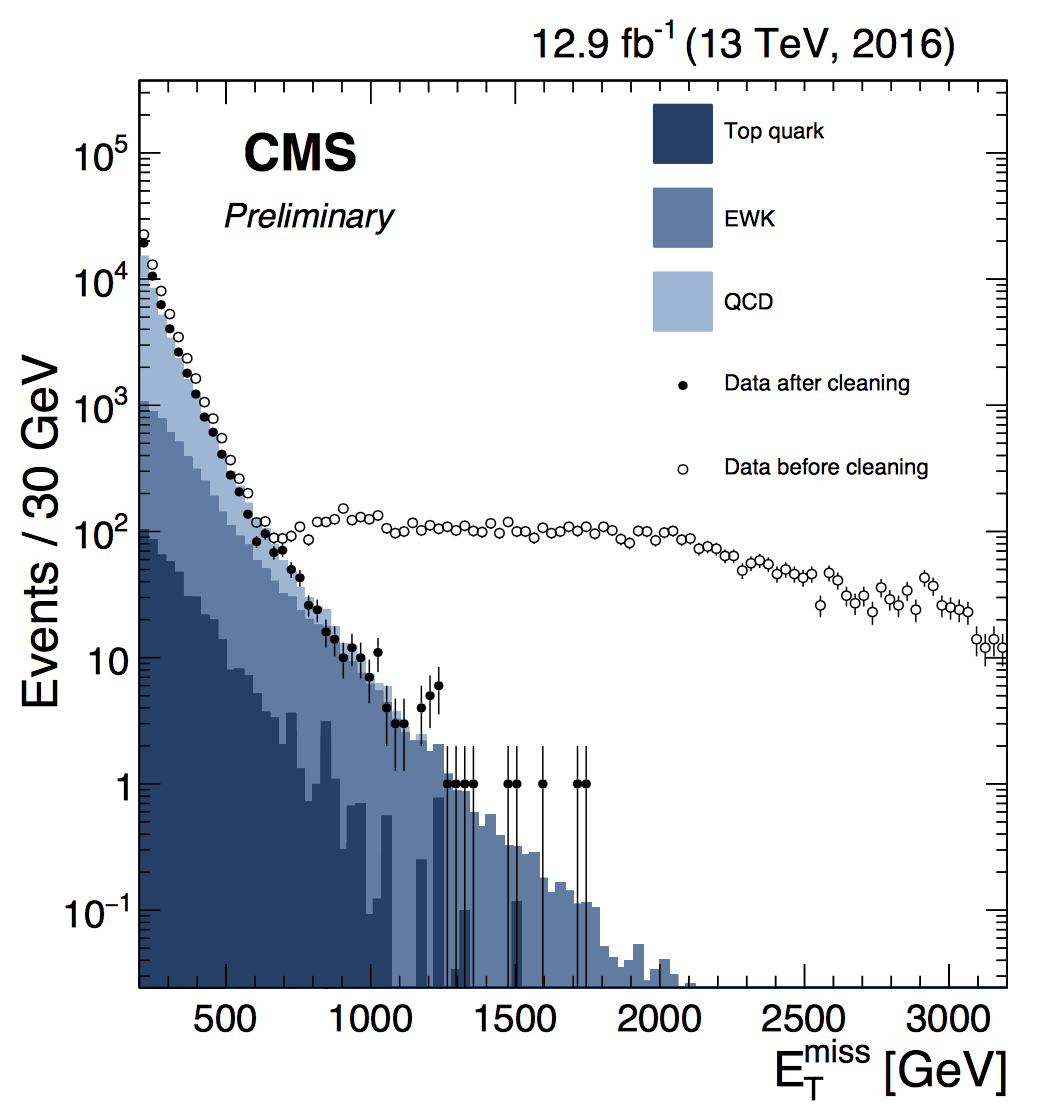
\includegraphics[width=0.5\textwidth]{figures/FakeMETTemp.png}
%Caption from the ATLAS monojet but they only have pT
%https://atlas.web.cern.ch/Atlas/GROUPS/PHYSICS/PAPERS/EXOT-2015-03/
\caption{The \MET distribution of the data events passing the [define selection] without any cleaning criteria applied on the leading jet. The Standard Model background indicated in the plots corresponds to the estimates obtained for the analysis signal region, including jet quality requirements. 
%The jet selection inefficiency of the cleaning selection is O(1\%), which is negligible compared to the observed excess in data. 
This demonstrates the necessity of a strong non-collision background suppression for this analysis. From~\cite{ToBeFound}.}
\label{fig:fakeMET}
\end{figure}

%CMS: up to 4 leading jets 
The CMS analysis also applies specific vetoes for photons and heavy flavour jets, to reject events with photon ISR or containing top quarks. The CMS analysis also includes a signal region targeting hadronic decays of the W and Z bosons using substructure techniques, which is considered separately in the case of ATLAS and will be discussed in Sec.~\ref{subsub:monoV}. 

\begin{marginnote}[]
\entry{Signal region}{a region of phase space for a search that is enriched in signal events. Event counts in this region are used to compare background-only prediction to data in search for discrepancies signaling new physics. 
%For example, a region with a high \MET and no other objects except for the ISR object is a signal region for a \MET+X search.
}
\entry{Control region}{a region of phase space for a search that is signal-free but with characteristics otherwise as close as possible to the signal region. Event counts in this region are used to estimate backgrounds in the signal region. 
%For example, a region requiring no \MET and a process mimicking that of the signal region is a control region for a \MET+X search.
}
\end{marginnote}


%%Backgrounds
The main background contributions that remain after the event selection are
invisible decays of the Z boson into neutrinos (approximately 55-70\% of the total background) 
%numbers in Livia's talk: https://indico.cern.ch/event/682235/contributions/2817876/attachments/1576792/2490208/DMWG-2017_V2.pdf and in Francesca's talk:
%https://indico.cern.ch/event/682235/contributions/2817877/attachments/1576793/2490236/171218_atlas_ungaro.pdf
and leptonic decays of the W boson where the lepton is not
reconstructed (approximately 20-35\% of the total background), in association with jets. 
%
In order to reduce theoretical and experimental uncertainties on the main V+jet backgrounds, the number of events in the signal region from each of these backgrounds are derived from data in signal-free \textit{control regions} selecting V+jet processes where the W and Z bosons decay into visible particles ($Z\rightarrow ll, W\rightarrow l\nu+jets$, where $l$ = $e, \mu$). 
%not sure we should say that the bin by bin estimates are used, here it's ambiguous
The event selection follows that of the signal region, substituting a lepton requirement to the lepton veto. The visible decay products in events selected for the control regions are subtracted from the total transverse momentum balance, providing an estimate of the contribution of these backgrounds in the signal region. CMS also uses a $\gamma$+jet control region where the photon is subtracted following the same procedure, to increase the statistical precision of the background estimate. 
%
The distribution of events in the main observable used for the search, the shape of the \MET distribution, is simulated and reweighted for each of the control regions using the most recent perturbative calculations for NLO QCD and QED~\cite{Lindert:2017olm}. The estimation of the number of $Z\rightarrow \nu\nu$events from the $\gamma$+jet and  $W\rightarrow l\nu$+jets control region needs a specific treatment due to the difference in the processes. This is particularly important for a consistent treatment of the different processes used in the background estimation and of the main theoretical uncertainties, and it will be discussed further in the following textbox. %CD: how do we call the thing
The full information on the theoretical and experimental uncertainties and their correlations from this procedure is used in a simultaneous fit to control and signal regions, to determine the overall background estimate in each of the \MET regions considered. 
%and leads to an improvement of 40 to 50% in the search according to PhilHarris and Livia, but I wouldn't add that unreferenced
Backgrounds from top processes in ATLAS are estimated using a dedicated control region with a requirement of a $b-$jet that is included in the fit, while CMS takes this background from simulation. Smaller diboson backgrounds are estimated from simulation. 

%Sidebar (50 words minimum, 200 words maximum) briefly discussing a fascinating adjacent topic; insert below Literature Cited section, but indicate near which section in text the sidebar should be typeset
\begin{textbox}[!h]
\section{Precision estimation of background for \MET+X searches}
In order to relate the number of events in the jet+\MET
signal regions (where $Z\rightarrow \nu\nu$ dominates) and control
regions (where events with jets produced in association with
$Z\rightarrow ll$, $W\rightarrow l\nu$ and $\gamma$ are used to maximise
the statistical power of the background estimation),
one needs to rely on a precise theory  
prediction of the ratio of the V+jets cross-sections. 
This is why this is important, this is 10 words. 
This is why this is important, this is 10 words. 
This is why this is important, this is 10 words. 
This is why this is important, this is 10 words. 
This is why this is important, this is 10 words. 
This is why this is important, this is 10 words. 
This is why this is important, this is 10 words. 
This is why this is important, this is 10 words. 
This is why this is important, this is 10 words. 
This is why this is important, this is 10 words. 
%\subsubsection{Precise background estimation}
%\label{sub:precision}

%Cite AR on this topi (but it's 2009): \cite{doi:10.1146/annurev.nucl.56.100704.122617}
%from ooutline
%- LHC results				
%	citations for most recent
%	- Differences between ATLAS and CMS:				
%		- CMS starts with only Z, ATLAS uses Z and W, CMS uses everything including gamma				
%		- theoretical issues with using Z and W				
%		- Pozzorini paper: shit is complicated, W and Z are one thing but if you want to do photon it's a different story				
%			- dependence of result on analysis cuts				
%			- QCD correction				
%			- EW corrections				
\end{textbox}

%%Experimental uncertainties
The systematic uncertainties on the background estimate for the jet+MET search range from 2 to 7\% (CMS) and 2 to 10\% (ATLAS), depending on the \MET region. The main uncertainties are due to the identification of leptons (CMS) and the understanding of the jet and \MET calibration (ATLAS). 

%%What it means for the models we talked about
Since no significant excess is found in any of the signal regions, limits are set on the parameter space of Higgs portal models described in Sec.~\ref{sec:HZPortalModels} and simplified models described in Sec.~\ref{sec:BSMMediatorModels}, namely where the SM-DM interaction is mediated by $s-$channel vector (V), axial vector (AV), scalar (S) and pseudoscalar (P) and colored scalar mediators.  
%CD: Maybe we put this in the reactions chapter? It is quite an important statement
Since the simulation of the entire parameter space for these models by the experiments is computationally intensive, the Dark Matter Forum had agreed on a limited set of benchmark parameters to be tested~\cite{Abercrombie:2015wmb}, privileging those that change the LHC kinematics of the search (e.g. give a harder \MET spectrum) rather than those that only change the cross-section of the process and can therefore be reinterpreted from the search results. For example, the kinematics and cross-section of the vector and axial vector mediators is very similar at the LHC, while the DD and ID cross-sections change. 
The parameter values used as benchmarks (e.g. couplings) have been selected considering the sensitivity of early Run-2 searches, precision constraints and general simplicity arguments. As described more in detail in Section~\ref{sub:comparisonVisibleInvisible}, results are given in the \mdm, \mmed  plane fixing the couplings to \gq=0.25 and \gdm=1.0 for vector and axial vector mediated models, \gq=\gdm=1.0 for scalar and pseudoscalar models and \gdmq=1.0 for colored scalar models. The simplified models employed by the experimental collaborations are known at NLO~\cite{Neubert:2015fka,Haisch:2013ata,Backovic:2015soa}. 

%monoH come from CMS but maybe ATLAS has a better reinterpretation. 
The most stringent 95\% C.L. observed (expected) upper limits on the invisible branching
fraction from jet+\MET searches are 53\% (40\%).  TODO look for ATLAS?
%(CMS, combining jet and vector boson radiation categories). 
%V/AV come from CMS search, ATLAS is less sensitive as it's 1.55 TeV
Vector and axial vector mediators are excluded by LHC searches at values of \mdm up to 700 and 400 GeV respectively with \mmed up to 1.8 TeV. This choice of model and couplings produces a relic density that is lower than the Planck measurement and it is still unconstrained by LHC searches for \mdm$>$0.3 TeV at \mdm$=$1.8 TeV for the vector mediator, and for 0.65$<$\mdm$<$0.75 TeV at \mdm=1.8 TeV for the axial vector mediator\footnote{Here and in the following, we quote observed limits at 95\% C.L. and refer to the bibliography for expected limits and 90\% C.L. limits.}. 
%CD: Not sure this is interesting for anyone? A bit complicated to project a 2D plot in words
%pseudoscalar comes from CMS
The LHC limit on the pseudoscalar mediator mass is lower due to the Yukawa-like couplings suppressing the cross-section with respect to spin-1 mediators, and it is 0.4 TeV in the CMS search for \mdm up to roughly 150 GeV. 
Jet+\MET searches are not yet sensitive to scalar mediators with the chosen couplings. 
%t-channel comes from ATLAS
%CMS
%Colored scalar mediators with masses up to 1.4 TeV at values of \mdm = 60 GeV are excluded.
%ATLAS
%CD TODO: check what parameters are people using?
Colored scalar mediators with masses up to 1.7 TeV at values of \mdm = 10 GeV are excluded for \gdmq=1 and \mdm=100 GeV. Considering this exclusion limit, this model still provides a viable DM relic density for \mmed \mdm above roughly 500 GeV at \mmed=1.7 TeV\footnote{The ATLAS and CMS results do not use the same parameters, here we report the ATLAS result.}.

Other benchmark scenarios such as compressed SUSY scenarios, 
%maybe explain?, 
squark pair production, 
%who ordered that
non-thermal singly-produced DM, 
and Large Extra Dimensions (ADD) are also constrained by the ATLAS and CMS searches, in some cases providing the most stringent constraints to date. 

%%Reinterpretation - this is the only thing that I think fits well here
The jet+\MET search can constrain a wide variety of reactions for invisible particles. Therefore, various approaches have been taken to allow model-builders and phenomenologists to easily reinterpret its results. As for most LHC searches, the published experimental data from the ATLAS and CMS collaborations is provided on the HEPData platform~\cite{Maguire:2017ypu}. Additionally, a  simplified likelihood function~\cite{Collaboration:2242860}, which under certain assumptions approximates the full likelihood using a reduced set of information, is provided for the CMS result~\cite{Sirunyan:2017jix} and has been used for reinterpretation~\cite{Pobbe:2017wrj}. Moreover, the ATLAS Collaboration has used the ratio of cross sections of events containing a jet and \MET and events containing a jet produced in association with an opposite-sign same-flavour dilepton pair from the decay of a Z/$\gamma*$ boson~\cite{Aaboud:2017buf}, corrected for detector effects. 
%in a fiducial phase space - saving space, leaving it unsaid
This is an observable sensitive to the anomalous production of events with jets and \MET, and uses many of the techniques from the the jet+\MET search described above to estimate background. The constraints derived are comparable to those of the jet+\MET search with the equivalent dataset. Unlike most other searches for new physics described in this review, detector effects are already accounted for (\textit{unfolded}) when presenting results, so that there is no need to implement a detector simulation to reinterpret this search. 

\subsubsection{Searches with photons and vector bosons}
\label{subsub:monoV}
%monophoton, monoV

Searches for invisible particles produced in association with a jet are the most sensitive among the searches employing an object radiated in the initial state, due to the large signal rates from the radiation of a gluon as opposed to the radiation of a photon or a W/Z/Higgs boson. The jet+\MET final state is however also affected by the largest SM and instrumental background, and only covers signals producing a high \MET to comply with data-taking limitations at the trigger level, due to the high-rate backgrounds producing signal-like signatures. It is therefore worth considering other objects as ISR, as those searches will be subject to different backgrounds, different kinds of systematic uncertainties, lower \MET thresholds, and can provide confirmation in case of an excess in the jet+\MET final state~\cite{Birkedal:2004xn,Petriello:2008pu}. 
%Gershtein:2008bf 2nd monophoton paper, save cites
The sensitivity hierarchy of \MET+X searches does not necessarily privilege the jet+\MET final state if there is a direct new physics coupling between a vector boson and the DM, as in the case of the EFT model mentioned in Section~\ref{sub:EFT}, or if the radiated object is a new particle~\cite{Autran:2015mfa}. 
%This latter signal motivates searches in the \MET+generic resonance final state CD: keep for later. 

ATLAS and CMS have pursued searches for missing transverse momentum produced in association with a photon%monophoton - if we're running low on citation space, remove CMS monophoton
\cite{Aaboud:2017dor,CMS-PAS-EXO-16-014},%less lumi, unpublished, ,
vector boson decaying hadronically %monoV, had, 2015+2016 (CMS) and 2015 (ATLAS)
\cite{Sirunyan:2017jix,Aaboud:2016qgg} or leptonically %monoV, lep, 2015+2016
\cite{Aaboud:2017bja, Sirunyan:2017qfc}. 

One of the advantages of these search signatures over the jet+\MET one
is the lower event selection threshold, thanks to the additional handles to suppress background
provided by either the photon ISR or the leptonic decays. As an example, the lowest \MET 
value for the search is 100 GeV for the leptonic Z+\MET search~\cite{Sirunyan:2017qfc} %CMS https://arxiv.org/pdf/1711.00431.pdf
as opposed to 200 GeV for the jet+\MET search~\cite{Sirunyan:2017jix}. 

%CD: this can be cut except for the first sentence? 
The event selection and the background estimation strategy depends on the final state, but generally mirror those of the jet+\MET search. 
The \textbf{photon+\MET searches} use a photon to trigger the events to be recorded for analysis, and selects events containing an isolated photon above 150 GeV and no leptons. The number of events from Z decays to neutrinos in association with a photon can be estimated in events where the lepton veto is inverted and the contribution of visible Z and W boson decays is removed from the transverse momentum balance of the event, and transferred to the signal region. The total systematic uncertainty is dominated by the statistical uncertainty in the control regions, ranging from 4\% to 10\%. 
%Don't want Zgamma resonances so restrict mllgamma < 1 TeV, but maybe too much info
Jets and leptons faking photons are estimated directly from data, and the $\gamma$+jet background where the jet is mismeasured and produced \MET is suppressed by the requirement that the photon and the direction of the \MET vector do not overlap in the azimuthal plane. 

%Total ATLAS uncertainty in SR1:
%post-fit
%>>> 160./2600
%0.06153846153846154
%pre-fit
%>>> 200./2400
%0.08333333333333333

The \textbf{W/Z+\MET searches} where the vector boson (V) decays to a quark-antiquark pair specifically select events where the decay products from the high-\pt{} boson are collimated, to better discriminate signal and background. QCD jets will not present any \textit{substructure}, while the decay products of vector bosons grouped into large-radius jets have a typical two-prong pattern from the hadronization of the quark-antiquark pair. The dominant background is still Z decays to neutrinos in association with jets, followed by W decays where the lepton is not identified, and top quark decays. The shapes of these backgrounds are estimated using simulation, while the normalization is determined in control regions, similarly to the jet+\MET search. In the CMS search, the V+\MET backgrounds are estimated in a simultaneous fit together with the jet+\MET backgrounds. The main uncertainty for this search (up to 9\%~\cite{Sirunyan:2017jix} and 13\%~\cite{Aaboud:2016qgg} %ATLAS, CMS is 9\% due to the tagging requirements
) is due to the modeling of the substructure observables. 
\begin{marginnote}[]
\entry{Jet substructure}{a set of techniques employed to extract information from the radiation pattern of a jet, by analyzing its constituents or its reconstruction history. For a review, see ~\cite{Larkoski:2017jix}.}
\end{marginnote}
The \textbf{Z+\MET searches} where the Z boson decays leptonically~\footnote{Leptonic decays W bosons have also been employed in the past for this kind of searches, but due to the additional experimental challenges (e.g. the presence of an additional invisible particle, the neutrino in the W decay) and the reduced sensitivity with respect to the hadronic decays, they have not been specifically pursued as DM searches for the LHC Run-2.} are sufficiently general to be sensitive to simplified models of DM with a Z radiation, as well as to Higgs decaying into new invisible particles and produced in association with a Z~\cite{Sirunyan:2017qfc, Aaboud:2017bja}. The event selection includes a constraint on the dilepton invariant mass, which limits the backgrounds to diboson, leptonically decaying top quarks, Drell-Yan production and a small amount of triboson processes. The estimation of the main $ZZ\rightarrow 2\nu 2l$ background (about 60\% of the total backgrounds) uses simulation, as the data sample that could be used to constrain the normalization as in the jet+\MET search is statistically-limited. The main uncertainty for this search (10\% on the background estimation) comes from the theoretical uncertainties on this background. The CMS search uses a Boosted Decision Tree (BDT) applied to events with the missing transverse momentum between 100 and 130 GeV, to enhance the sensitivity to invisible Higgs decays. 

The photon+\MET searches provide the next-to-most stringent constraints after the jet+\MET search, 
up to \mmed $<$ 1200 GeV for vector and axial vector mediators with \gdm=1.0 and \gq=0.25 for \mdm=100 GeV,
in the region where the mediator can decay to DM. %Not mentioning off-shell, otherwise it's a closed region. 
The ATLAS photon+\MET search also sets limit on the EFT model where the DM couples directly to the photon, 
excluding EFT scales between 150 and 750 GeV for \mdm=100 GeV, assuming the maximal coupling value allowed by perturbativity. 
%The excluded region decreases to 150-600 GeV for a coupling value of 3. 
Searches in the \MET+hadronic Z final state constrain vector and axial vector mediator
masses of \mmed $<$ 650 GeV for \mdm=100 GeV\footnote{As a side note that is useful to compare results from different LHC datasets, 
Run-1 V+\MET searches used a version of the vector simplified model
that enhanced W radiation because of the constructive interference 
due to different up- and down-quark mediator couplings,
but that was not gauge invariant~\cite{Bell:2015sza,1475-7516-2016-01-051}.}. 
Searches in the \MET+leptonic Z final state provide constraints on 
\mmed $<$ 650 GeV for \mdm=100 GeV for vector and axial vector mediators. 
W/Z+\MET searches are also uniquely sensitive to the radiation of a boson 
from the mediator particle in the case of colored scalar models~\cite{Bell:2012rg}, 
but the Run-2 searches do not present this interpretation. 
%CD: maybe we add a link to the 8 TeV search but it's worse than monojet 

\subsubsection{Search signatures including the Higgs boson}
%monoH, H to invisible detailed earlier on

%CD: we already said that before
The newly discovered Higgs boson is of particular interest for DM searches at the LHC. 
Higgs radiation is kinematically and PDF suppressed, but searches for a mono-Higgs have
other strong theoretical motivations. 
Higgs portal models are the simplest incarnation of theories where the coupling
between the dark sector and the SM is realized through a Higgs boson. Higgs couplings
to at least a new scalar are necessary for the gauge invariance of simplified models described in
the previous chapters towards more complete theories. 
%The rates of signatures including Higgs bosons are small, but 
Gauge symmetries link Higgs+\MET signatures and signatures including W, Z bosons
or jets as well as two-body mediator searches~\cite{Liew:2016oon}. 
%so results from Higgs searches are not to be taken in isolation.  

The search strategy depends on the decay mode of the Higgs boson. 
With the current LHC dataset (2015+2016 Run-2, 36 $fb^{-1}$), only the 
$H \rightarrow \gamma\gamma$ and $H \rightarrow b\bar{b}$ decay channels 
have been used to search for DM, due to their relative experimental simplicity
and high rates. Other decay channels such as $ZZ, WW$ and $\tau\tau$ are 
expected to contribute to DM searches as well in the future. 

Searches in the decay channel 
$H \rightarrow \gamma\gamma$ in association with \MET~\cite{CMS-PAS-EXO-16-054,Aaboud:2017uak}
are sensitive to a variety of benchmark models regardless of the small branching fraction, thanks to the 
high precision in the reconstructed Higgs boson mass and the ability to probe low \MET 
thresholds compared to other Higgs decay channel as the trigger rates are low. 
The SM background is estimated using a fit to the diphoton mass distribution, in events categorized
according to their missing transverse momentum for CMS (50$<$\MET$<$130 GeV and \MET$>130$ GeV)
or according to specifications optimised for different signal categories.%this is useless but the analysis is needlessly complicated  
The main uncertainty for the $H \rightarrow \gamma\gamma$ searches using the 2015+2016
LHC Run-2 dataset is statistical. 
In the search where the Higgs boson decays into two bottom quarks~\cite{Aaboud:2017yqz}
in association with \MET$>$150 GeV, 
all backgrounds except for the QCD background are estimated using MC simulation
and constrained in dedicated control regions. This search also employs jet substructure
techniques for events with \MET$>$500 GeV,
to discriminate boosted Higgs decays from QCD processes. 
The main systematic uncertainty for the lower \MET signal region is the modelling 
of the V+jets background, while higher \MET signal region is still statistically limited
with the 2015+2016 LHC dataset.

In absence of discrepancies between data and background,
limits are set on the baryonic Higgs benchmark model outlined in
Sec.~\ref{sub:simplifiedModels} with 
\gq=1, \gdm=1, \ghZprimeZprime/$m_{Z}$=1, \sinthetab=0.3, 
%CMS: mZ'=10-10000 GeV, mDM=1-1000 GeV
%CD: it would be nice to say what this can be reinterpreted to but we have no space
and on a Z'-2HDM model with $tan\beta$=1, \gZPrime=0.8 and \mdm=100 GeV~\footnote{ 
In the case of the Z'-2HDM model, CMS and ATLAS set different masses for the 
new Higgs bosons, 
%https://docs.google.com/presentation/d/10R9XJaoMDEhXKhd_Wx9yMXEaPl4uXR8IcmuTeLancvg/edit#slide=id.g1f308da957_0_17
%ATLAS fixes both to 300 GeV, CMS fixes to mA0 
%For the record:
%CMS: A and Z' varied between 300-800 and 600-2500 GeV respectively
%ATLAS: mZ? = 400 to 1400 GeV, mA0 = 200 to 450 GeV
%The masses of the neutral CP-even scalar (H0) and the charged scalars (H�) from Z?-2HDM model are set to 300 GeV. The DM mass m? is set to 100 GeV 
%CMS: 
%Two-Higgs-doublet-Z' signals with a pseudoscalar mass of 300 GeV are excluded at 95\% CL for Z' masses below 900 GeV
%Baryonic Z' models with a dark matter mass of 1 GeV are excluded at 95% CL for Z' masses below 800 GeV
so the constraints are not directly comparable. 
This has been rectified in the coming iteration of these analyses.}. 

%CD: I kinda want to say this but we have no space so why bother
%the mandala boson is shit, misguided attempts at combining Higgs discovery with every other excess

\subsubsection{Searches with heavy-flavor quarks}
%ttbar+MET
%reinterpretation of SUSY

Generic searches employing one single additional object produced in association with \MET
are powerful tools to probe simple models of DM. More complex models, however, bring 
more handles for discovery: the first step in this direction can be taken with searches using 
scalar and pseudoscalar models as benchmarks, where information about the production mechanism 
(e.g. the mediator is produced in association with two heavy flavor quark, complementing the
gluon-fusion production mode of the \MET+jet searches) is exploited in 
the search strategy. 

The searches in~\cite{Aaboud:2017rzf,CMS-PAS-EXO-16-051}
are optimized for DM scalar and pseudoscalar mediators
selecting events in the semileptonic and fully hadronic top quark decay channels,
as well as events containing one or two bottom quarks, in association with \MET. 
The dominant backgrounds in~\cite{Aaboud:2017rzf} are estimated separately
using MC in each of the signal regions,
and their normalization constrained using control regions in a simultaneous fit.
The main uncertainties for these searches are, depending on the signal region, 
theoretical and MC simulation related uncertainties, jet energy scale and resolution. 
and uncertainties related to the identification of heavy flavor quarks. 
Signatures including \MET and two heavy flavor quarks are similar to 
signatures of third generation quark superpartners, leading to dedicated
DM signal regions being included in SUSY searches or used
for reinterpretation~\cite{Aaboud:2017aeu,CMS-PAS-SUS-17-001}. 
In SUSY-like searches, the dominant $t\bar{t}$ backgrounds
are heavily suppressed using variables that combine visible and invisible
mass~\cite{Lester:1999tx} targeting the model sought. 
This step uses information that is model-dependent,
but increases the sensitivity to specific processes. The remaining
small backgrounds are estimated using simulation. 

The sensitivity of searches of \MET associated to top quarks
is comparable for the two strategies. 
For a choice of \mdm=1 GeV, pseudoscalar mediator masses of 10-50
GeV~\cite{AAaboud:2017aeu} and scalar mediator masses up to 100
GeV~\cite{CMS-PAS-SUS-17-001} are excluded. 
%CD: it would be nice to find out why this difference in sensitivity? 
The increased LHC dataset 
will allow these searches to be sensitive for other DM masses. 
%CD: this sentence is shit but i'm tired
Signatures with $b\bar{b}$ pairs are less sensitive to
scalar and pseudoscalar mediators that do not explicitly
privilege bottom quarks. Mediator masses for the b-flavored colored scalar 
model discussed in~\cite{Agrawal:2014una} are excluded up to 1.1 TeV
for \mdm=35 GeV. 

%Not spending more than one sentence on monotop, is that ok?
Other searches in the heavy flavor+\MET category are those only
including only one top or bottom quark
(also called mono-top or mono-bottom searches)~\cite{CMS-PAS-EXO-16-051, Aad:2014wza},
and place constraints on models that include singly-produced DM candidates
through flavor-changing neutral currents, described in~\cite{Boucheneb:2014wza}. 

%The main backgrounds for these searches are single top or misidentified $t\bar{t}$ processes. 
%The search where the top quark decays hadronically
%employs substructure techniques to tag the boosted top quark decays.  
%These searches place constraints on models of DM (resonant, non-resonant). 

\subsubsection{Two-body mediator searches}
\label{sub:twoBody}
%Dijet and dilepton
%Mention TLA

Decays into pairs of SM particles are an inevitable consequences of models where
DM mediators are exchanged in the $s-$channel and have a SM coupling. 
This possibility to probe the SM-DM interaction through the visible 
decays of mediator is a unique feature of collider experiments
%and can be exploited for dark boson models as well? 
and one that they are well-prepared for, with a wealth of generic searches for
two-body resonances (see e.g.~\cite{Harris:2011bh}).
In the following, we will describe two of the most general examples,
the searches for dijet and dilepton resonances, their challenges and the implication of their results
for models of SM-DM mediation. % including a Z'-like mediator. 

%Describe dijet search
\textbf{Searches for dijet resonances} exploit the smoothness of the falling QCD background
to derive their background directly from a fit to data. This minimizes modelling
and theoretical uncertainties. Localized excesses are sought atop %woo atop!
the fitted background estimation~\cite{Aaboud:2017yvp,CMS-PAS-EXO-16-056}. 
%Where dijet lose sensitivity: wide signals, angular 
If the resonance is wider than 15\%, as in the case of 
vector and axial vector mediator models with couplings roughly above \gq$>$0.5~\footnote{This value
assumes that the new particle can decay only to quarks and DM particles, with \gdm=1.0 and \mdm=1 GeV.}, 
the fitted background estimation will be biased by the presence of signal. 
In this case, the \textbf{scattering angle of dijet events} can be exploited as a discriminating variable, 
since the QCD background is dominated by $t-$channel processes that privilege
large angular separations between the two jets, as opposed to signals with an isotropic angular distribution
in the center-of-mass frame that translates to the presence of more central jets in the
detector~\cite{CMS-PAS-EXO-16-046,Aaboud:2017yvp}.  
%$s-$channel scattering processes are more in the center-of-mass frame
%are not 
%in case of wide resonances, 
%and below the trigger thresholds .  

%Where dijets lose sensitivity: low-mass 
Standard LHC dijet searches lose sensitivity at masses below the TeV, where the high QCD
rates force the experiments to randomly discard a large fraction of background and
signal events alike (see sidebar). %sidecar, not sure how to call this but we can ask for help
An example of such a technique is recording only \textbf{partial event information} for later analysis directly 
from the trigger system (called Data Scouting in CMS~\cite{CMS-PAS-EXO-16-056},
Trigger-object Level Analysis in ATLAS~\cite{Aaboud:2016leb}, Turbo Stream in LHCb~\cite{Aaij:2016rxn}),
to overcome the data storage constraints. 
Dijet resonance searches that use this technique~\cite{CMS-PAS-EXO-16-056,ATLAS:2016xiv}
can record the full rate of dijet events to much lower dijet invariant masses than the standard dijet
searches, but have to overcome a number of challenges that go beyond
a seemingly simple search. The first challenge is demonstrating that the
performance of the physics objects reconstructed at the trigger level is sufficiently good
to perform a physics analysis and not just take a decision on whether to keep the event.
Secondly, the extremely large background rates (above 10$^5$ events/GeV) grant
a sufficient statistical precision to observe signals of the order of a few thousand events,
but also per mille-level detector and SM contamination effects. 
An alternative data-taking strategy is to require a \textbf{high-\pt{} ISR object} to trigger
on the event and reduce the QCD background, but the sensitivity is reduced by this requirement with
respect to selecting the leading order dijet process. The ISR object can be either a jet and a photon,
and it recoils against a dijet pair. The dijet pair can be either resolved~\cite{ATLAS:2016bvn} or
collimated and reconstructed within a large-radius jet tagged with substructure techniques~\cite{Sirunyan:2017nvi},
depending on the ratio between mass and transverse momentum of the resonance
that boost the decay products. If the mediator particle decays democratically to
different quark flavours or preferentially into heavy flavour quarks (as in the case for a scalar mediator),
searching for \textbf{$b\bar{b}$ or $t\bar{t}$ resonances}~\cite{lowMassDiB,CMS-PAS-HIG-16-025} 
can overcome the data taking constraints 
at masses above roughly 500 GeV and have a sensitivity comparable to inclusive 
dijet searches for vector and axial vector mediators. An interesting feature of 
scalar and pseudoscalar particles decaying to $t\bar{t}$ 
is their interference with SM $gg \rightarrow t\bar{t}$ production~\cite{Djouadi:2016ack}
that has to be explicitly accounted for when estimating the background for these searches
~\cite{Aaboud:2017hnm}. 

TODO: add coupling-mass summary plot for ATLAS
%TLA and challenges, point to sidebar

%Sidebar (50 words minimum, 200 words maximum) briefly discussing a fascinating adjacent topic; 
%insert below Literature Cited section, but indicate near which section in text the sidebar should be typeset
%Consider swapping with the ERC text below?
\begin{textbox}[!h]
\section{Challenges in selecting events at the detector level (trigger)}
%Trying to approximate 10 words per line
%Notes for improvement: 
%this is too long, needs sharpening. 
% the points i want to make are:
% higher thresholds are bad for mediator searches and also in general -> go TLA
% pileup increases MET thresholds -> get track info at the trigger level
%it needs a much clearer motivation: model X gives low mass. 
%probably that needs done in the text because space constraints, but then why using this box-thing (other than tidying things up)? 
The LHC collides protons every 25 $\mathrm{ns}$, producing 40 billion 
of events per second at nominal conditions. This amount of data cannot be 
recorded in its entirety, and not all events are interesting
for the experiments' physics programmes. %programmes or programs?
A trigger system is used to decide whether an event is selected for further analysis. 
Its first level is realized in hardware and only uses
partial detector information for fast decisions in a time of
the order of $\mathrm{\mu s}$, while its second level is software-based
and uses more refined algorithms and information to make a
decision in $\mathrm{ms}$. 

\textbf{Challenge: triggering on low-\pt objects}
Since the rates of SM physics processes decrease
with the transverse momentum of the objects involved, and processes
with a high momentum transfer have a higher chance of containing
interesting features or new particles, the trigger system records
events above a certain threshold e.g. in leading jet \pt or in event \MET. 
Only a fraction of events that do not satisfy these thresholds is recorded. 
Searches for signals with high-rate backgrounds and 
MET or jet \pt below these thresholds are 
therefore penalized unless novel
%not novel anymore?
data recording techniques, such as only recording partial event information 
needed for the search, are employed.

\textbf{Challenge: \textit{pile-up} in trigger} Simultaneous proton-proton interactions occurring within the detector
readout time cannot be completely disentangled from the hard process
of interest, especially if reconstructing the collision vertex
is not possible at the trigger level due to CPU constraints. 
This \textit{pile-up} increases the likelihood of passing 
the minimum threshold to record events, especially in the \MET triggers.
For this reason, the increase in the LHC instantaneous luminosity by virtue
of increasing the number of simultaneous
collisions leads to increases in the trigger thresholds to
keep manageable event recording rates. Reconstruction algorithms that suppress
the effects of pile-up can be employed by ATLAS and CMS directly at the trigger level,
using information on the objects and energy density within the event~\cite{CMS:2014ata,ATLAS-CONF-2014-019}. 
In future LHC runs, track information to disentangle the provenance of the 
energy deposits from the collision vertex will be available for
ATLAS and CMS from dedicated hardware systems (see e.g. Refs.~\cite{Shochet:2013gaw,1748-0221-6-12-C12065}). 
\end{textbox}

%Describe dilepton and remind of why we want to include dilepton
Searches for new particles decaying in opposite-sign, same-flavor lepton pairs~\cite{Aaboud:2017buh,Khachatryan:2016zqb} can also be interpreted in terms of the simplified models of DM, 
if the mediator particle has sizable couplings to leptons. Although lepton couplings
are not mandated by the quark-antiquark production at hadron colliders as dijet couplings are, 
lepton couplings feature in a variety of models that can embed
the simplified models of DM used as benchmark for LHC searches. %this sentence repeats the one in Sec.2. 

The main backgrounds for the dilepton searches in electron and muon final states 
arise from Drell-Yan processes, and are estimated using simulation corrected for NNLO effects and normalized to the Z boson peak event yield in data. 
%ATLAS. too much detail
%The background prediction is smoothed using functional fits where the number of simulated events is not representative of the data statistics. 
Reducible backgrounds where other objects are mismeasured as leptons are estimated using data. The main uncertainties on the background estimation are of theoretical nature, for the entire invariant mass range. 

%List constraints from both searches with two coupling options
%The CMS analysis also scans the coupling-mass plane by fixing the ratio between \mdm and \mmed to ensure perturbativity 
%CMS sentence: Quark couplings down to 0.05 for mediator masses at 50 GeV are excluded for the spin- 1 simplified models as shown in Fig. 12. 
The same constraints from dijet and dilepton searches apply to both vector and axial vector mediators:
the LHC phenomenology (rates and kinematics) is the same for both. Searches for visible mediator decays 
are sensitive to masses as low as 50 GeV (boosted dijet) and constrain SM-DM couplings \gq as low as 
0.05 at 60 GeV. Jets from the mediator decay start being spatially separated above mediator masses of 250-300 GeV, 
and that is where the resolved dijet+ISR topology takes over in terms of sensitivity, with the $\gamma$ ISR + dijet channel
constraining \gq$>$0.15-0.2 up to 350 GeV, where the jet ISR + dijet channel is not limited by
trigger thresholds anymore and is more sensitive due to the higher gluon radiation rates.
Searches with jets at the trigger level are the most sensitive to low-mass mediators where available,
excluding simplified models with \gq as low as 0.05 starting from 400 GeV. 
Standard dijet searches constrain models with DM mediators up to 3 TeV.  
%but lose sensitivity to lower couplings where they start to be statistically limited. 
Dilepton searches are more sensitive than dijet searches in case of equal couplings
of the mediator to leptons and jets, due to the much reduced backgrounds. ATLAS and CMS searches
with the 2015+2016 dataset probe signal masses starting from 150 and 400 GeV respectively.  
%what is the minimum coupling by dilepton searches? not sure this is easy to do without reinterpretation

%Mention LianTao's paper where baryonic / 2HDM monoHiggs is also constrained. 
%Mention results of other searches: ttbar resonances for pseudoscalar with interference, Higgs-like scalars (CMS boosted) 

\subsubsection{Comparison of sensitivity of visible and invisible LHC searches}
\label{sub:comparisonVisibleInvisible}

It is important to note that generic searches for new two-body resonances
are by design sensitive to a broad range of theoretical benchmarks, 
and as such they alone can offer little information on 
whether a discovery would imply in terms of DM mediators.
In absence of a signal and within a specific model scenario,
searches for mediator particle with visible decays
provide constraints that are complementary to those of searches
for DM particles, in particular in the off-shell region 2\mdm $>$ \mmed where the mediator
cannot decay to DM directly but can still decay into much lighter SM particles
such as leptons and quarks. 
The relative sensitivity of the two kinds of searches
is a model- and parameter-dependent statement: for $s-$channel simplified models
searches for DM particles only dominate if the coupling to DM is much larger
than the coupling to quarks, and even then reducing \gq reduces the LHC production
cross-section and therefore the overall sensitivity of \MET+X searches. 
One advantage of searches for invisible particles is their sensitivity to models with
very light mediators ($<$50 GeV), since the reach of dijet and dilepton searches to low-mass
resonances is still ultimately limited by data taking constraints. 

%Mention why we plot things in the mass-mass plane. 
A sketch of the comparison of the sensitivity of searches for visible decays of vector and axial vector mediator models, and invisible DM particles 
in the \mdm vs \mmed plane is shown in Fig.~\ref{fig:sensitivityComparison}, fixing the couplings. The choice of plane and the scenarios chosen follow the choices of the Dark Matter Working Group~\cite{Albert:2017onk}, to illustrate the complementarity of different LHC searches for $s-$channel-mediated model of DM and to convey the message that the sensitivity of LHC searches to simplified models of DM depends both on model choice and parameter choice. 
%Mention why mass-mass? Because on-shell/off-shell regions clearly spelled out

The topmost left-hand side figure shows a leptophobic vector mediator with \gl=0, \gdm=1.0 and \gq=0.25, where dijet searches for visible decays of the mediator constrain both on-shell and off-shell region but are limited by data-taking constraints at masses above roughly 50 GeV, where \MET+X searches take over in the on-shell region. An equivalent picture is drawn for the vector mediator, in the top right plot. The bottom right plot shows the case of an axial vector mediator with reduced quark couplings and equal lepton couplings (\gq=\gl=0.1 and \gdm=1.0), where it can be seen that searches for dilepton resonances cover a larger range of parameter space with respect to dijet resonances but are still limited at low mediator masses; the region constrained by from \MET+jet searches extends to lower DM and mediator masses with respect to the case of the model with \gq=0.25 due to the reduced production rate. The third panel in the bottom left shows the scenario of a vector mediator where lepton couplings are reduced with respect to quark couplings (\gq=0.1, \gl=0.01, \gdm=1.0), where the range of all regions constrained by visible mediator decay searches is considerably reduced with respect to the scenarios with larger couplings. 

%TODO: make more visible, limit to 2 plots
\begin{figure}[!htpb]
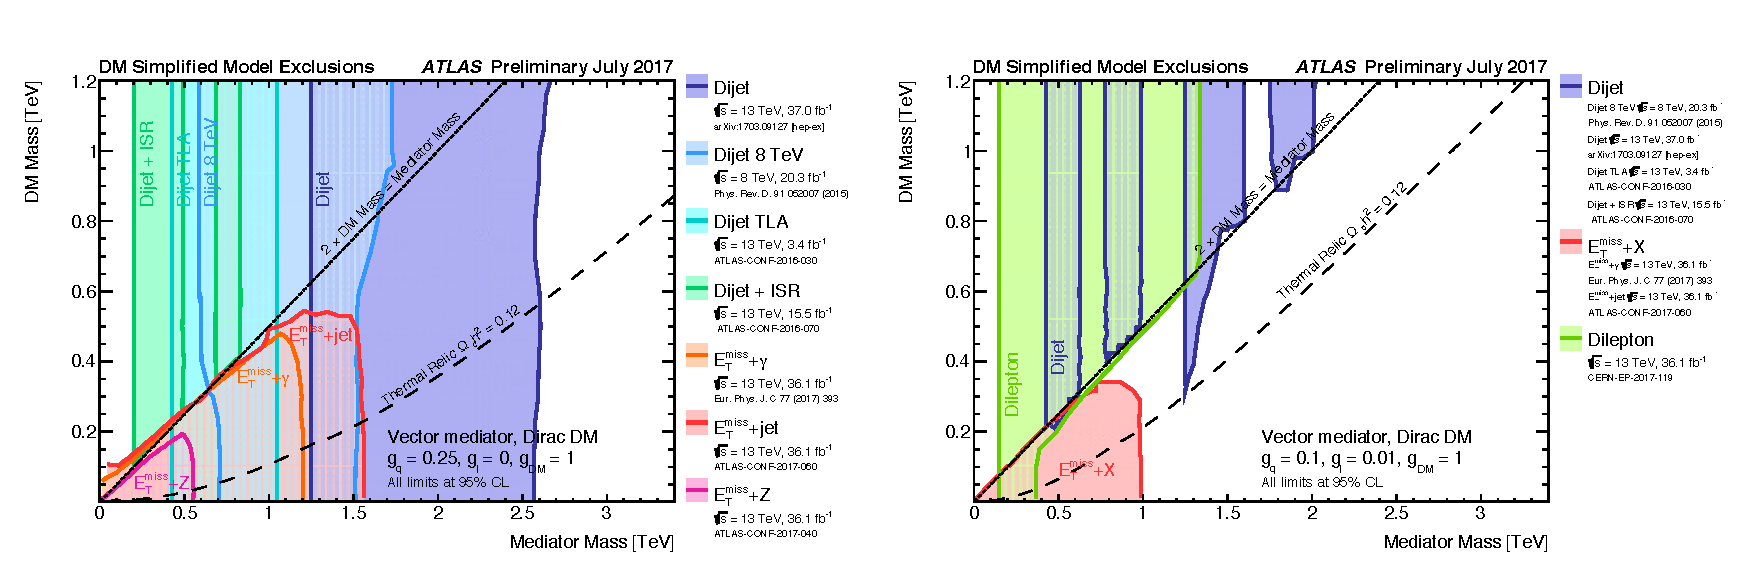
\includegraphics[width=\textwidth]{figures/SummaryPlotsMassMass.pdf}\caption{
Regions in a dark matter mass-mediator mass plane excluded at 95\% CL by a selection of ATLAS dark matter searches, for a vector mediator benchmark model with varying coupling scenarios. Top plots: \gq=0.25, \gl=0.0, \gdm=1.0, axial vector (left, separate search constraints) and vector mediator (right, combined search constraints), highlighting the sensitivity of visible searches in this scenario and the near-equivalence of the vector and axial vector as benchmark models for LHC searches. Bottom plots: \gq=0.1, \gl=0.1, \gdm=1.0 for an axial vector mediator (left) and \gq=0.1, \gl=0.01, \gdm=1.0 for a vector mediator (right), highlighting the sensitivity of the lepton searches and its dependence on the chosen coupling value. Dashed curves labeled "thermal relic" indicate combinations of dark matter and mediator mass that are consistent with a dark matter density of $\omega_c = 0.12 h^2$ and a standard thermal history, as computed in MadDM~\cite{Backovic:2015cra}. The dotted curve indicates the kinematic threshold where the mediator can decay on-shell into dark matter. }
%\gdm=1.0  \gq=0.25universal to all flavors, and a lepton coupling gl set to zero. This choice of couplings corresponds to the "V1" scenario in arXiv:1703.05703. Leptonic decays are absent at tree level. The results use 13 TeV data except for Phys. Rev. D91 052007 (2015). The exclusions from the ATLAS dijet searches are derived from the limits provided on Gaussian-shaped resonances following the procedure recommended by ATLAS in Appendix A of Phys. Rev. D91 052007 (2015) and in arXiv:1703.09127. Small fluctuations in the contour are a product of the dijet reinterpretation scheme. 
%To the left of the curve, annihilation processes described by the simplified model deplete ?c below 0.12 h2. A dotted curve indicates the kinematic threshold where the mediator can decay on-shell into dark matter. The exclusion regions, relic density contours, and unitarity curve are not applicable to other choices of coupling values or model.
\label{fig:sensitivityComparison}
\end{figure}

%CD: if we want coupling-mass, we could show the plots in the figs dir: SummaryPlotsCouplingMass.pdf

%In case sample figure with different scenarios as an example
%\begin{figure}[!htpb]
%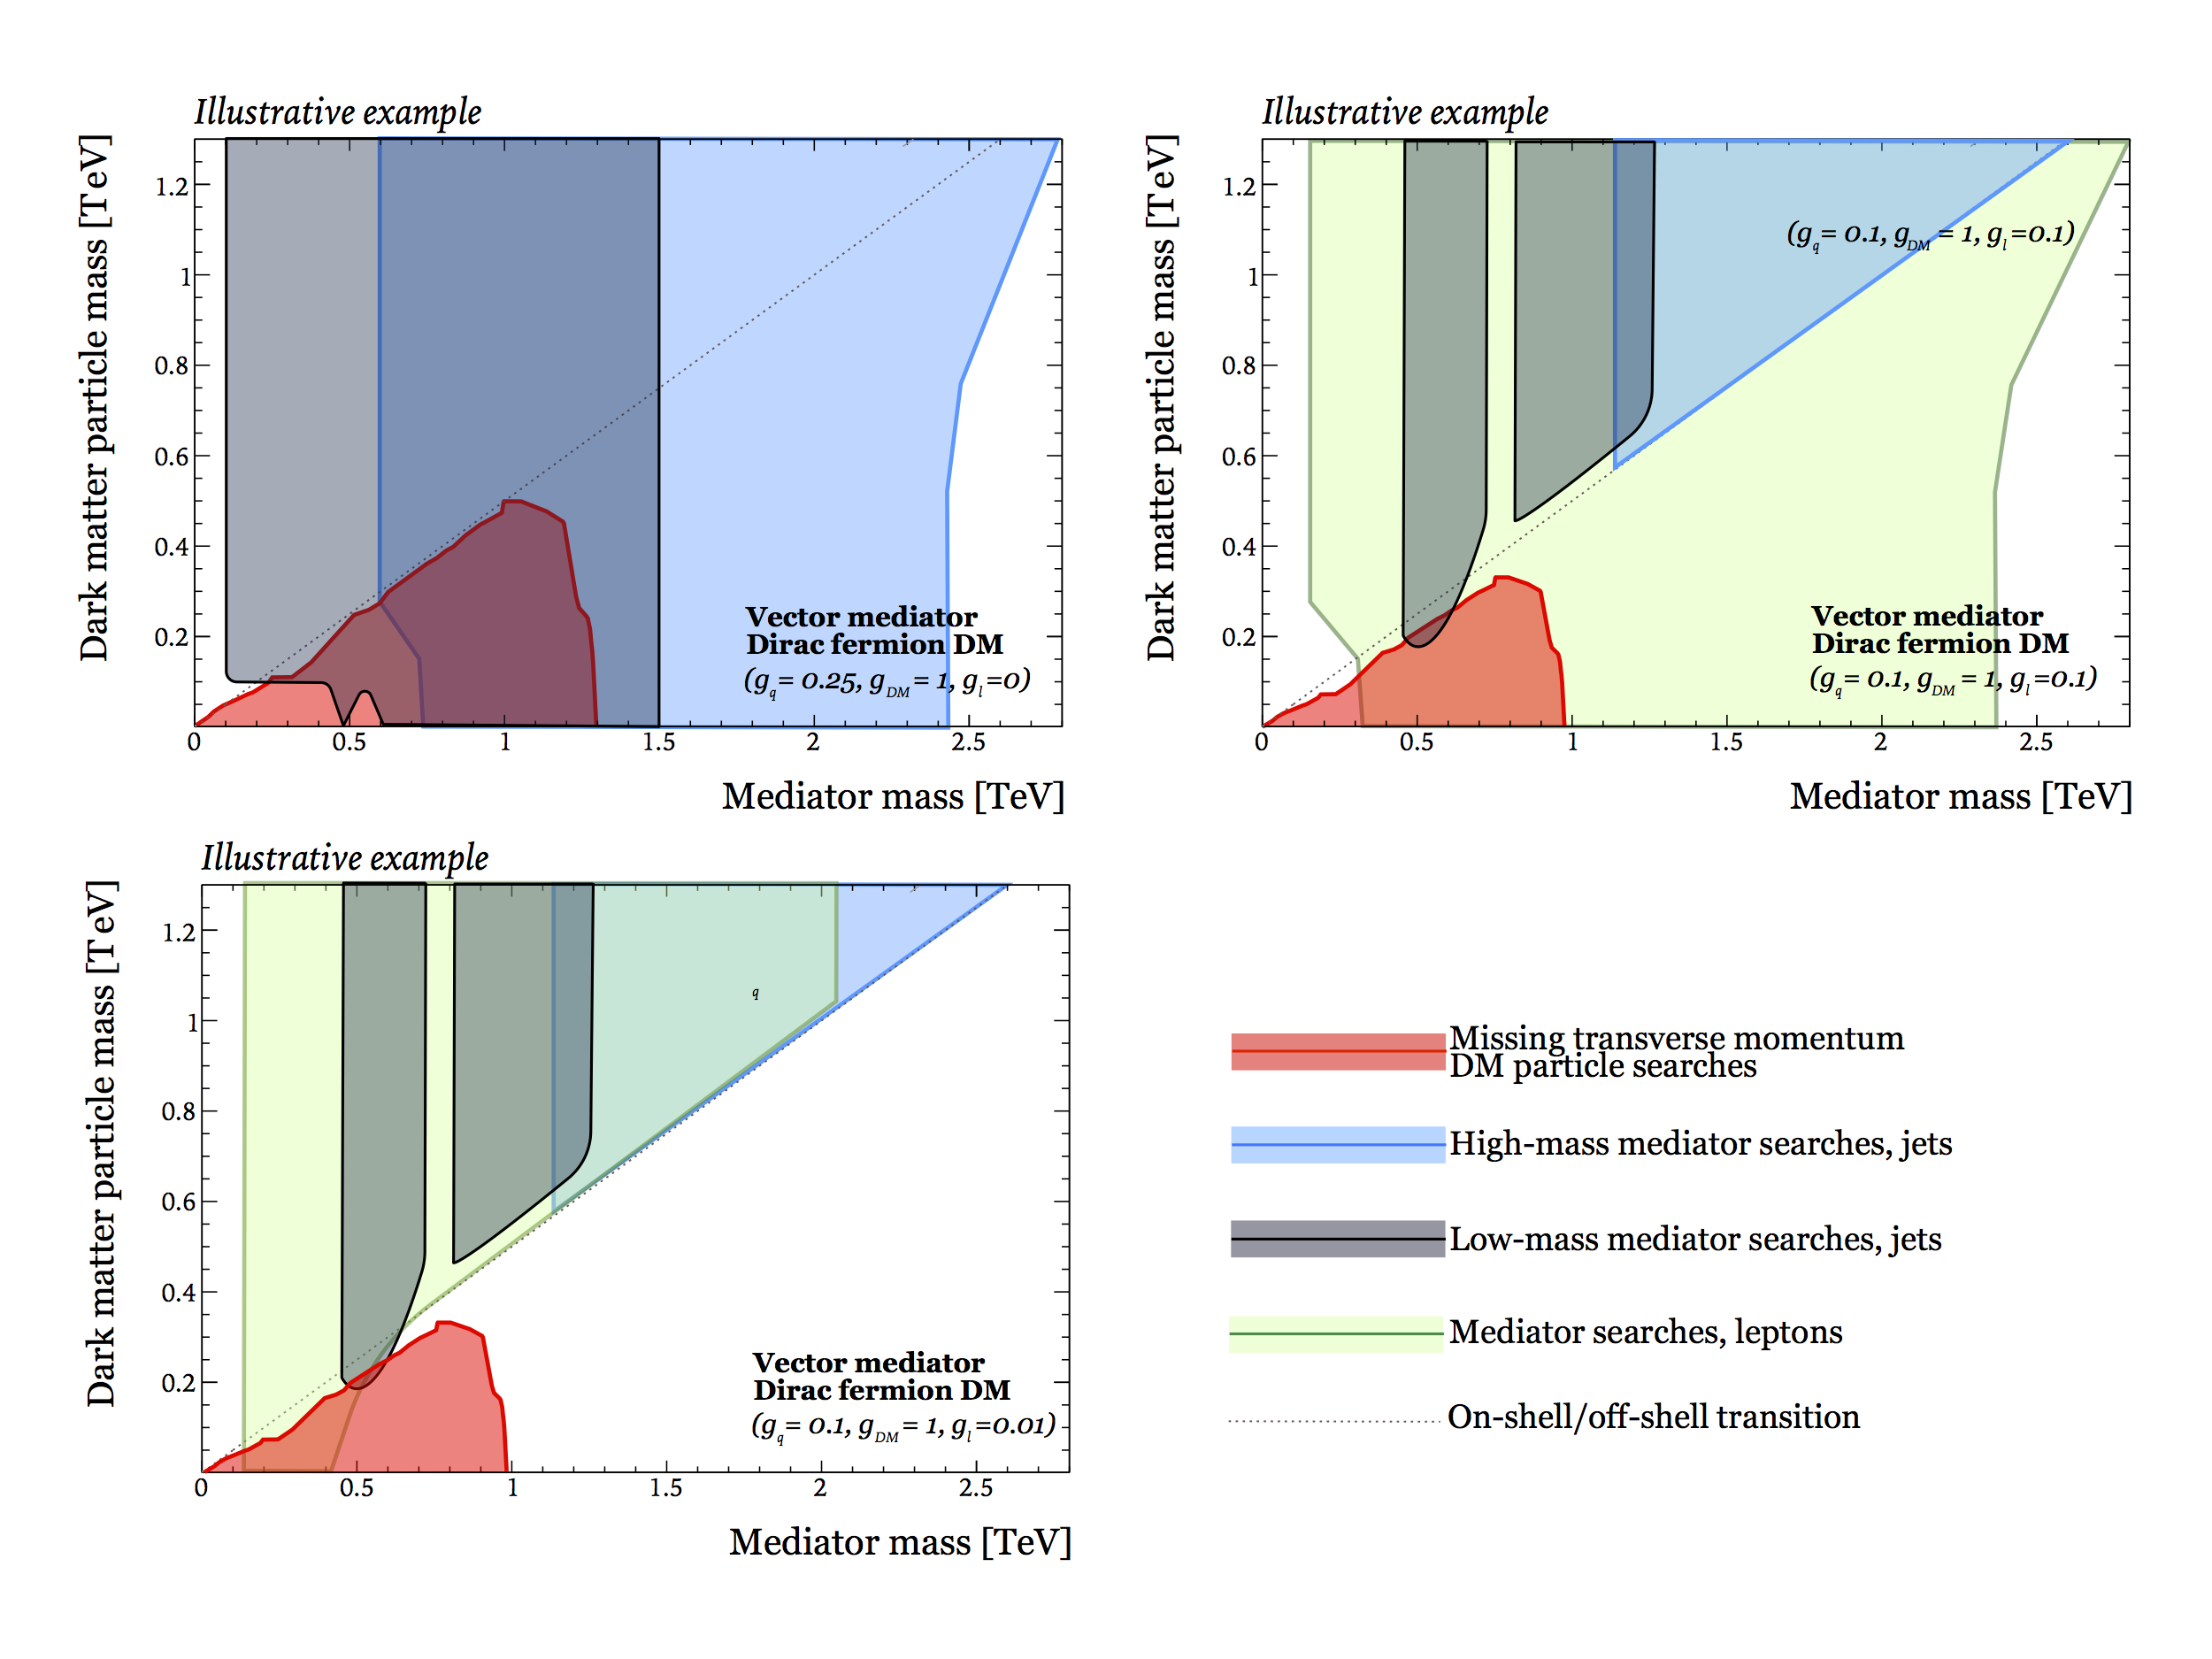
\includegraphics[width=\textwidth]{figures/DMSummary.png}
%\caption{Illustrative examples of the comparison of the sensitivity of searches for visible and invisible mediators in the \mdm-\mmed plane, for different coupling scenarios. No actual data has been used, but experimental observations have been used as inspiration for the figure. From~\cite{AnotherWikipedia}.}
%\label{fig:sensitivityComparison}
%\end{figure}

%It would be nice to make tables of lowest mediator/DM searches+refs for 100 GeV DM mass,
%as a poor-person approximation of a summary plot we can't make because ATLAS data not public. 

%%%SUMMARY TABLE FOR MONOX SEARCHES: descoped, unless we just want a list of references of all the searches which may be useful but obsoletes early
%\begin{table}[h]
\tabcolsep7.5pt
\caption{Summary of searches for BSM mediators at the LHC}
\label{tab:BSMSearchesSummary}
\begin{center}
\begin{tabular}{@{}l|c|c|c|c@{}}
\hline
Signature & Model& \mmed limit & \mdm limit  & Cit.\\
 &  & (\mdm=100 GeV) & (\mmed=100 GeV)  &  \\
%{(}units)$^{\rm a}$ &Head 2 &Head 3 &Head 4 &{(}units)\\
\hline
Jets+\MET & $s-$channel, AV$^{\rm a}$ & Column3 & Column4 & \cite{Sirunyan:2017jix,Aaboud:2017phn} \\
Jets+\MET & $s-$channel, V$^{\rm a}$ & Column3 & Column4 & \cite{Sirunyan:2017jix,Aaboud:2017phn} \\
Jets+\MET & colored scalar & Column3 & Column4 & \cite{Sirunyan:2017jix,Aaboud:2017phn} \\
Photon+\MET & Column 2 & Column3 & Column4 & Column\\
W,Z (had)+\MET 1 & Column 2 & Column3 & Column4 &Column\\
W,Z (lep)+\MET 1 & Column 2 & Column3 & Column4 &Column\\
Higgs+\MET &Column 2 & Column3 & Column4 &Column\\
\hline
\end{tabular}
\end{center}
%\begin{tabnote}
$^{\rm a}$ Coupling values: \gq=0.25, \gdm=1.0; $^{\rm b}$second table footnote.
%\end{tabnote}
\end{table}



\subsection{Searches for SUSY DM}
\label{sec:results_SUSYSearches}
%Good talk for ATLAS:
%http://cds.cern.ch/record/2299118/files/ATL-PHYS-SLIDE-2017-1008.pdf
%SUSY2017 summary
%https://indico.cern.ch/event/695201/contributions/2853913/attachments/1582877/2502678/011618_SUSY17Summary.pdf

SUSY Dark Matter is a well-motivated search target of collider searches, and as such it has received 
large experimental attention, demonstrated in the numerous searches published by ATLAS and CMS alone since the start of the LHC.  
In this section we only give a flavor of the most recent experimental results, concentrating on those
that specifically highlight the connections to cosmological observables. 

As discussed in Sec.~\ref{sec:SUSYModels}, predictive benchmark models lead to specific signatures
where the DM particle (often leading to \MET) is accompanied by a cascade of other objects. 
The presence of invisible particles in the final state prevents the reconstruction of the full decay chain, and 
searches often use discriminating variables that are a proxy of the combined mass of visible and invisible
particles in the event (see e.g.~\cite{Lester:1999tx}). 
If a search addresses specific final states in its signal regions,
then it will benefit from an increased sensitivity with respect to a more generic \MET+X search
designed to lay hold of a number of less specific models.  
For this reason, SUSY searches apply a more stringent event selection for their signal regions than generic searches. 
The cost of this increased sensitivity is a larger number of possible searches that must be done to have a
broad coverage of the various specific possibilities in which new SUSY particles would manifest. 

%CD question: do we want to talk about the search methodology, VR, CR, SR? I would say no but it depends on what we do with the monojet part. 
Many SUSY searches use simplified model as benchmark signals. These models are usually inspired by restricted versions of the
MSSM and capture the kinematics of only a subsection of the particle spectrum. Simplified models can subsequently be combined to constrain
full, self-consistent models~\cite{Kraml:2013mwa}. Search results are presented in the plane of neutralino mass against superpartner particle mass.
This is the same strategy adopted 
%this is not to piss off Oliver otherwise I'd write it the other way around because I am Italian and I like sentences that start with a clause
by generic DM searches. 

R-parity conserving SUSY searches can be broadly categorized
%this way we're not going to talk about RPV? but not sure this apply, see RPV gravitino
according to the features of the signal they would produce at colliders, specifically whether:
\begin{itemize}
\item the new particles sought are strongly or weakly produced, leading to decay chains containing strongly or weakly interacting SM particles; %strong SUSY and weak SUSY 
\item heavy superpartners of the top and bottom quarks are present, leading to final states with heavy flavor quarks;%Stop and 3rd gen
\item whether the particle spectrum of LSP and NLSP is compressed, leading to either soft or long-lived objects. %LLP SUSY
\end{itemize}

\begin{figure}[!htpb]
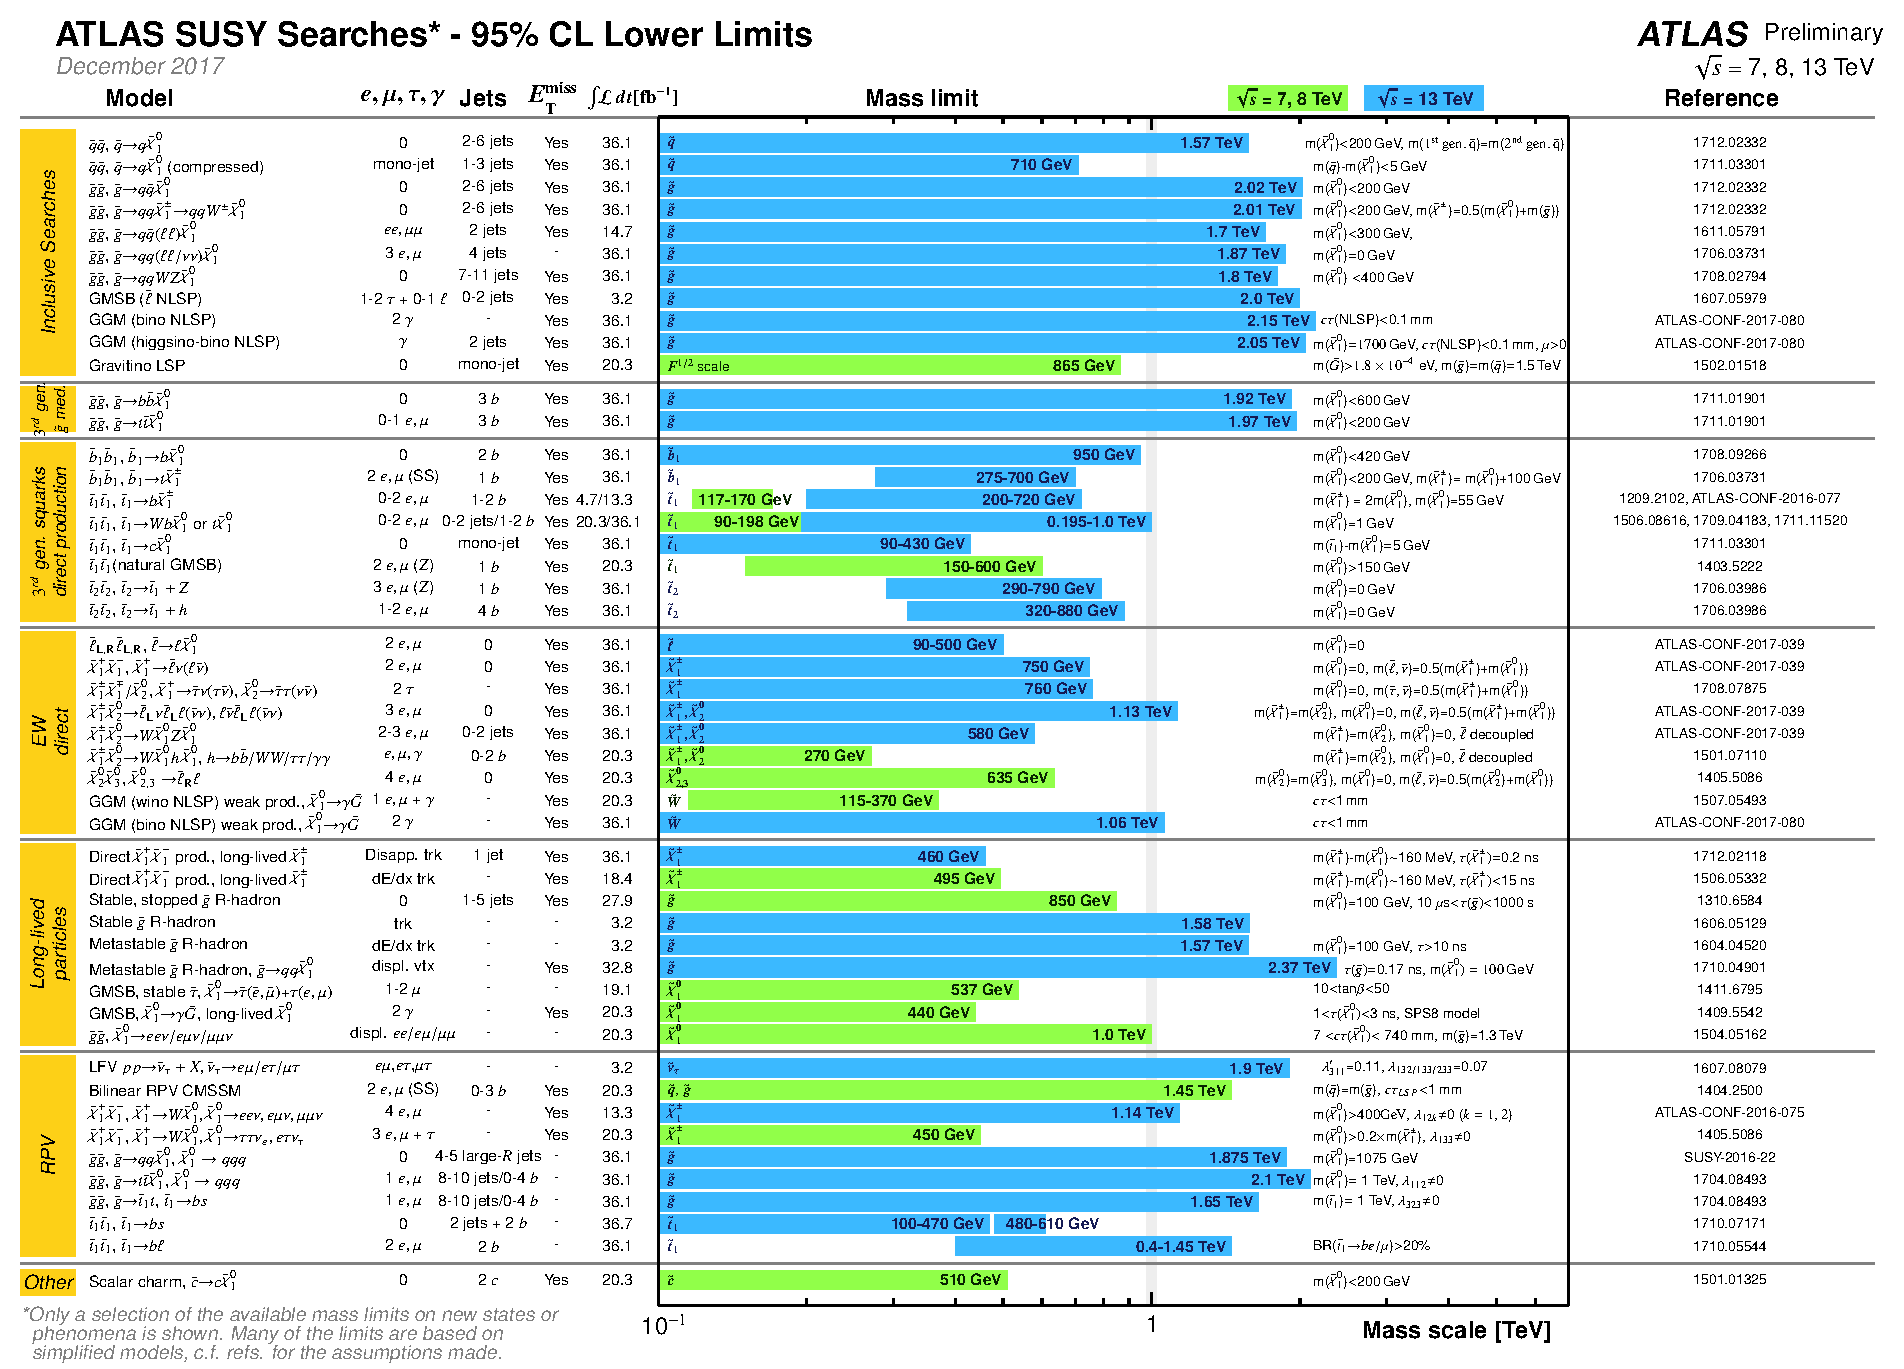
\includegraphics[width=\textwidth]{figures/ATLAS_SUSY_Summary.pdf}
\caption{Mass reach of ATLAS searches for a representative selection of results available in December 2017. From~\cite{ATLASSUSYSummary}.\label{fig:SUSYSummary}}
\end{figure}

No SUSY search so far has found evidence for the discovery of new particles, and the mass
reach of ATLAS searches using simplified models is shown in Fig.~\ref{fig:SUSYSummary}, with a similar reach for CMS searches. 
The lower limit on the masses of the strongly produced partners of quarks and gluons %for 100 GeV neutralino masses
are approaching 2 TeV (see e.g.~\cite{Aaboud:2017bac}). 
%picked the strongest gluino limit from https://atlas.web.cern.ch/Atlas/GROUPS/PHYSICS/CombinedSummaryPlots/SUSY/ATLAS_SUSY_Strong_all/ATLAS_SUSY_Strong_all.png
Heavy flavor supersymmetric partners are excluded below 1 TeV (see e.g.~\cite{Sirunyan:2017wif}). %picked the latest stop 0L from CMS
Weakly coupled SUSY models have much smaller cross sections with respect to their strongly coupled counterparts, 
and require larger integrated luminosities for discovery or exclusion, the combination of a variety of searches 
as in [SUS-17-004, CMS combination] or specific signatures, e.g. requiring a highly energetic jet to the search
region to select events regardless of the low \MET from compressed spectra as in [SUSY-2016-025] or
by exploiting the long lifetime arising from the small mass difference between the particles in the decay chain
[PUB-2017-019, reinterpreted]. %CD: This is poor effort but do we want to give it more space? 
The searches for gauge boson superpartners (gauginos) have a reach of approximately 1 TeV if the superpartners
of SM leptons are light and the search can benefit from a high leptonic branching ratio, 
while the constraint on the gaugino masses reduces to 600 GeV if their decays proceed
through W and Z bosons.
%Maybe we shouldn't call them gauginos because that is more terminology? 

%Notes from the SUSY talk
%No evidence for Jet+MET SUSY (strong plain SUSY)
%Specifically target scenarios of gauge mediated: add photons to the final state and push sensitivity
%SUSY 2017 Gluino up to 2 TeV range. 
%There are parallels between the models
%Use exclusive combinations of objects
%Pick the right signal, very specific also in the mass spectrum 
%RPV: gravitino DM 

%Higgsino searches nice to find projections for those. going to take a lot of luminosity.

%\subsubsection{pMSSM scans}

Targeting a specific signature, such as a cascade decay in a specific SUSY simplified model, 
drastically increases our ability to discover it. A narrower focus however trades generality for sensitivity. 
Designing and interpreting searches solely using simplified models may not capture the spectrum of possibilities
given by full, theoretically well motivated models. 

The concreteness of SUSY can be put to use to complement simplified models, by mapping search design and
interpretations to many different combinations of parameters in a full model such as the pMSSM. 
Ref.\cite{Conley:2010du}, and continuing through LHC experiments ~\cite{Aad:2015baa, Khachatryan:2016nvf},
use the pMSSM to define a finite (though large) parameter space to probe. In this context, 
one can ask, systematically, what regions of the parameter space are already excluded by
existing results and what regions remain viable. 
%, and why those regions have so far remained untouched. %CD: unclear how you can tell this from SUSY scans?

Even the approach of these scans does not provide rigid or exhaustive exploration of the possibilities,
as even the pMSSM relies on simplifying assumptions, but these efforts can provide a coarse-grained
map determining signatures that remain unexplored by current searches.  
Adding assumptions relating the LSP to a thermal relic, one can further narrow the list of search
targets and key in on particular regions of parameter space for prioritized studies, see e.g. Ref.~\cite{Aaboud:2016wna}
in the case of electroweak SUSY. 
%CD: I would leave this discussion for the relic section later. Otherwise we can start with:
%These assumptions are of course not to be taken as more than a guiding principle... 

Tools such as Mastercode~\cite{Bagnaschi:2017tru} and GAMBIT~\cite{Athron:2017ard} can also be used to fit SUSY (and generic BSM)
model parameters to data and cosmological constraints. The outcome of these codes, often ran on supercomputers, 
is the likelihood for the viability of sets of parameters of a SUSY model given the available data from
colliders and other experiments.
%CD: I am not 100% sure I can convey this in three lines.

%global fitting code for generic Beyond the Standard Model theories, designed to allow fast and easy definition of new models, observables, likelihoods, scanners and backend physics codes.
%code that allows to fit different versions of the Minimal Supersymmetric Standard Model (MSSM) to currently existing experimental data.


%(cite battaglia etc? and ATLAS paper with relic?). Mention that these assumptions are of course very tenuous,
%as they deal with physics at potentially much higher energy scales. But DM density is one
%of the only clues we have about BSM, so more, not less, of this sort of thing is interesting to do (i.e. vary the assumptions).

%Other tools to do this. GAMBIT.

%Tools exist to approac

%\subsubsection{Models with long-lived particles}
%This serves as transition for the LLP chapter


\cite{Cahill-Rowley:2014twa} %???


\subsection{Searches for DM in association with long-lived particles}
\label{sec:results_LLPSearches}

%TODO: transition from NLSP talk above (which e.g. could be metastable and long lived) to talking about the exotics/general counterpart to susy.

%summary diagram in https://indico.cern.ch/event/656211/contributions/2673379/attachments/1498650/2333150/UW_dark_photons.pdf

The LHC searches mentioned in this chapter, with the exception of compressed SUSY scenarios, 
so far target prompt production of WIMP DM or associated mediator particles at colliders. 
The absence of a signal constrains these traditional WIMP models to have small cross-sections and high mass scales. 
This is one of the reasons why less-accessible dark photon models, including mediators with masses from the MeV to the tens
of GeV and with a range of potential lifetimes, are a target that is gaining interest by LHC searches. The list of results
below is only an example of LHC searches for dark photons to exemplify the upcoming opportunities for these signatures at colliders. 

These signatures are particularly challenging for ATLAS and CMS, given that many of these possibilities escape
conventional detection (e.g. decay outside the tracking volume, requiring custom reconstruction techniques, or 
are too light to be selected by the trigger). 
Collider experiments can still search for distinctive detector signatures from visible decays of light dark bosons. 
The searches in~\cite{ATLAS:2016jza} look for \textit{lepton-jets}, collimated decay products of light,
long-lived boosted dark bosons.
%Prompt also exists, see Miriam's diagram
The BR of the SM Higgs boson is found to be below 10\% for a range of masses and lifetimes. This search benefits from tailored
trigger and reconstruction algorithms for collimated muons. Other examples of searches for dark photons at
general purpose experiments are exotic decays of the Higgs boson~\cite{Aad:2015sva.CMS-PAS-HIG-16-035}, 
where dark bosons are pair-produced and decay to muons. 
%The CMS mass range covered is 0.25-8.5 GeV, while the ATLAS range is 15 and 60 GeV
%Lepton-jets are also produced in SUSY cascade decays. 
%https://indico.cern.ch/event/492240/contributions/2302157/attachments/1367524/2072266/Leptonjets_HiggsCoupling_Nov2016_Safonov.pdf
%fun substructure for electron jets
%https://journals.aps.org/prd/abstract/10.1103/PhysRevD.95.055007
%If we want to mention sterile neutrinos (probably not), https://journals.aps.org/prd/abstract/10.1103/PhysRevD.91.093010
Drell-Yan dilepton production
and electroweak precision observables are also sensitive to these models~\cite{Curtin:2014cca},
due to the mixing of the dark boson with the SM bosons. 
%Mention sensitivity? See Shelton's talk
The LHCb experiment can exploit precise tracking 
to search for visible decays of both prompt and long-lived dark boson into muon pairs~\cite{Aaij:2017rft},
providing the most stringent constraints between 10 and 70 GeV. 
Only visible decays are accessible to LHCb,
it is a non-hermetic forward experiment. 
Experiments at electron-positron colliders, such as the BaBar and Belle experiments, 
exploit the knowledge of the center-of-mass energy as a constraint to compensate their non-hermeticity, 
and set stringent collider limits on the kinetic coupling $\epsilon$ for this kind of models
for dark boson masses between 0.5 and 10 GeV. 


%%%%%%%%
%ASSORTED JUNK
%%%%%%%%

%beginning with the searches that illustrate many of the experimental 
%
%
% and then signals of MET. 
%
% description has a historical and ordering
%We begin with introducing 
%
%start with introducing the searches, mostly  
%
% of DM searches, we will turn to a [categorization] of the searches done so far. After a summary of searches for interactions through SM bosons, we turn to the experimental results 


%As described in the previous chapter, DM itself is not visible at colliders and has
%to be observed indirectly in association with other visible particles. 
%
%Signals of DM can come from MonoX and diX searches. 
%
%State of the art MC:
%
%Vector and scalar models are known at NLO~\cite{Neubert:2015fka,Haisch:2013ata}
%NLO corrections for vector and scalar models in monoZ and monojet
%
%t-channel
%
%From Millie's talk (see Reaction OmniOutliner):
%Since the DM-mediator-quark vertices allow for simultaneous FS partons with different hard scale, particular prescription needs to be used for the generation of samples with different partons that splits samples in number of mediators. Interference between the diagrams is neglected following Papucci et al. 

%%%Bunch of text from ERC that could be useful for TLA part

%This is what I wrote in ERC, not sure if it's usable

%At the LHC, proton beams with a center of mass energy of 13 \tera\electronvolt \ will collide up to 
%every 25 \nano\second \ at the four interaction points, where experiments are installed. 
%The ATLAS (\textbf{A} \textbf{T}oroidal \textbf{L}HC \textbf{A}pparatu\textbf{S}) experiment 
%is a general purpose detector located at the Interaction Point 1.
%From the Spring of 2010 to Fall 2012 the LHC has recorded a total of 25 \invfb of collision data 
%at 7 and 8 \tera\electronvolt. 
%
%It is the high interaction rate of proton-proton collisions at the LHC that 
%allows the collection of the large dataset necessary to search for rare processes. 
%The design and operation of the ATLAS detector is described in 
%References~\cite{DetectorPaper}. The key subsystems employed in this projects are the calorimeters, 
%where energy deposits from the collimated sprays of particles originated by 
%quarks and gluons are detected. The energy deposits are used as inputs of 
%\textit{jet algorithms}~\cite{Salam:2009jx}: 
%the experimental output used for the analysis is a reconstructed jet that, after calibration, 
%contains information on the kinematics of the original physics process. 
%The system and technologies employed to select and collect interesting data are the crucial components for the 
%innovative Trigger Level Analysis searches outlined in WP2 and WP3, 
%and they are described in more detail in Section~\ref{subsub:datacollection}. 
%
%The LHC will restart operations in Summer 2015, increasing the center of mass energy to 13 TeV. 
%The dataset collected over the course of the planned three years of operations (called \textit{Run 2}, 
%ongoing until mid-2018) corresponds to 100 \invpb~\cite{KEKRossi}. 
%Upgrades to further increase the data rate and the center of mass energy to 14 TeV will be 
%undertaken during the course of 2016, and completed during the 1.5 year technical stop (called LS2).
%LS2 will last until the beginning of 2020, leading to the third LHC run 
%that will collect an additional 200 \invpb of data. 
%
%During LS2, the LHC experiments will undergo major upgrades to their hardware (called Phase-I upgrades). 
%In the final two years of this project that coincide with the LHC Run 3, 
%I will exploit the new gFEX trigger board~\cite{Bartoldus:1602235} to extend the Trigger-Level Analysis 
%method to obtain an increased sensitivity for four-jet final states. 
%
%\subsubsection{Data collection and data analysis in ATLAS at the LHC}
%\label{subsub:datacollection}
%
%The rare signal events sought are buried in an overwhelming number of background events.
%It is therefore necessary to have a \textit{trigger} system that in a very short timescale 
%selects the interesting collision events based on the presence of high transverse momentum physics objects 
%(muons, electrons, photons, jets and tau leptons). 
%
%The ATLAS data collection rate at the end of the trigger selection still
%surpasses other ``Big data'' 
%challenges both in academic research and in industry. 
%As an example, ATLAS and the three other main detectors at the LHC produced and recorded 
%13 petabytes of data just in 2010~\cite{NaturePetabyte}. It is clear
%that with such large dataset new ideas and new analysis techniques are needed,
%especially in the case of small deviations over large backgrounds. 
%One such idea consists of moving the data analysis as close
%to the data taking as possible, ultimately removing the need for storage at all. 
%This proposal moves the first steps for the ATLAS detector in this direction, 
%proposing to only retain a subset of the event information, and eventually 
%to move an entire search to be done in real-time as soon as the data
%is collected. 
%
%\paragraph{The ATLAS Trigger system}
%
%The ATLAS trigger system is subdivided in two levels: Level-1 and High Level Trigger (HLT)
%The first, fast selection is made at L1 using coarse detector information. 
%Its logic is mostly hardwired in the readout electronics, 
%given that the decision needs to be made in less than 2.5 $\mu$ \second. 
%The bandwidth available for data transfer to the HLT and the HLT computing power
%limit the rate that could be accepted by the L1 to 75 kHZ from the initial 40 MHz 
%provided by the LHC~\cite{Sfyrla:1510140}. The events accepted by the L1 trigger 
%are passed on to the HLT trigger, a software subsystem. The longer latency allows 
%to perform a more refined reconstruction of the objects that are used for the selection.
%Jets reconstructed within the HLT system will be called \textit{trigger jets} in the following,
%while \textit{offline jets} are those reconstructed after the event has passed the full trigger chain.
%During the 2012 data taking, ATLAS recorded and reconstructed data at a rate of 
%400 Hz, leaving an additional 200 Hz of recorded data for later reconstruction
%(\textit{delayed} data).  
%
%Since the rate for certain signatures (e.g. multi-jet events that are backgrounds of the 
%searches outlined in this proposal) would saturate the limited bandwidth that needs to be shared 
%by all triggers, some triggers are \textit{prescaled}. 
%This means that only a fraction of the events accepted 
%are effectively passed onto the next level.
%A prescale of 1 means that all events 
%selected by the trigger are accepted, while larger prescales mean that only a fraction 
%1/prescale is accepted. This in turn harms the sensitivity of searches, as signal events
%will be rejected by the trigger system as well. 

%Blurb from ERC

%Hadronic jets are a particularly promising final state for both the Dark Matter mediators 
%produced at the LHC, but also for new, unknown particles that might be created when crossing 
%the threshold of a new energy scale such as in the upcoming LHC run. 
%Not knowing the exact nature of these new particles, it is not possible
%to pin down at which energy scales they are going to be produced, 
%and at which rates. This calls for generic searches that are sensitive 
%to a broad range of theoretical benchmarks, and whose results can be easily
%re-interpreted in different frameworks. The absence of any New Physics discoveries 
%during the first LHC run also points to the need for the study of more elaborate 
%and rare processes that can only be achieved with new analysis techniques. 

%A wide range of theoretical models attempt to incorporate Dark Matter. 
%Many of these models postulate the presence of a new massive subatomic particle
%that interacts only feebly with SM particles as a Dark Matter candidate.
%The presence of these Weakly Interacting Massive Particles (WIMPs) can be inferred in 
%in a variety of experiments. \textit{Direct Detection} 
%experiments detect the interaction between an incoming 
%Dark Matter particle and target nuclei within the detector, by measuring nucleon recoil.
%\textit{Indirect Detection} experiments detect the fluxes of SM particles that 
%are produced from the annihilation of DM particles~\cite{Bertone:2004pz, Bauer:2013ihz}. 
%Dark Matter searches at colliders are supported by the consistency
%of the thermal relic density and the annihilation rates of WIMP candidates with masses
%in the GeV-TeV range, compatible with the energy regime of the LHC~\cite{Bertone:2004pz}. 
%The complementarity of those searches in terms of the WIMP-SM interaction of interest 
%is shown in Figures~\ref{fig:complementarity} (a-c). 
%
%\begin{wrapfigure}{L}{0.7\textwidth}
%% \begin{figure}[!h]
%\centering
%    \includegraphics[width=0.65\textwidth]{figures/SimplifiedModels}
%  \caption[Complementarity of DM searches]{\label{fig:complementarity} Sketch showing the complementarity 
%  between different experiments searching for Dark Matter (a-c). The difference between
%  the EFT approach and the simplified model approach is depicted for collider searches in (c-d).}
%% \end{figure}
%\end{wrapfigure}
%
%Indirect detection experiments such as 
%FERMI~\cite{Hooper:2010mq}, AMS 
%~\cite{PhysRevLett.113.121101} and DAMA~\cite{Bernabei:2003za}
%have observed tantalizing signals 
%with a possible Dark Matter explanation.
%There some tension between direct detection experiments: the signal-like excesses 
%and characteristics of events in the CDMS and CoGENT experiments~\cite{Agnese:2013rvf,Hooper:2010uy}
%are not confirmed by other experiments such as LUX~\cite{Akerib:2013tjd}. 
%
%The flagship searches for Dark Matter at the LHC and at the Tevatron 
%exploit the recoil of undetected pair-produced WIMPs against a jet radiated 
%by one of the initial-state quarks or gluons. Such searches have yet to find 
%evidence for WIMPs (see e.g. Refs. ~\cite{Aad:2013oja,ATLAS:2014wra,Aad:2014vka,Aad:2014vea,Aad:2014tda,ATLAS-CONF-2012-147}
%for the ATLAS Collaboration). 
%
%Results from all these experiments need to be connected in a coherent framework for a 
%successful program of study of Dark Matter in the coming years. 


\section{EXTRAPOLATION OF COLLIDER RESULTS}
\label{sec:04_Extrapolation}
Models of particle dark matter involving SM-DM interactions necessarily link searches for DM at collider and searches in direct and direct detection experiments. Figures~\ref{fig:Complementarity} (a-c) show that, in the EFT paradigm, different search strategies are simply looking at the same process from different perspectives: DM can interact in the lab in DD experiments, it can be observed in space %galaxies is too close to snowmass formulation "indirect detection experiments that connect lab signals to dark matter in our own and other galaxies"
by ID experiments, and it can be created in the lab by colliders and observed by experiments such as ATLAS, CMS and LHCb. This complementarity of multiple experiments is necessary to elucidate the nature of dark matter in case of a discovery. Collider experiments are unable to determine whether a new phenomenon with the signatures discussed in Sec.~\ref{sec:03_ExperimentalResults} are directly connected to DM processes. % from an invisible particle or from a DM mediator. 
%Good sentence from DMF 
%One advantage of collider experiments lies in their ability to study and possibly characterize the mediator. A discovery of an anomalous E/T signature at the LHC would not uniquely imply discovery of dark matter, while at the same time e.g. discovery of an anomalous and annually-modulated signal in a direct-detection experiment would leave unanswered many questions about the nature of the interaction that could be resolved by the simultaneous discovery of a new mediator particle. Collider, direct, and indirect detection searches provide complementary ways to approach this problem [50], and it is in this spirit that much of our focus is on the mediator.

On the other hand, collider experiment can make a prediction for the signal strength of a particular model and test its consistency with relic density. This prediction can be verified in presence of a signal in DD and ID, and the connection with the galactic nature of the new phenomenon can be established. Colliders can also shed light on the physics processes that complement DM production, e.g. as in Fig.~\ref{fig:Complementarity} (d) colliders can discover the new particle mediating the interaction and measure its coupling to SM particles other than quarks and gluons, or they can observe other cascade decays that produce the DM particle in case of SUSY models. For this reason, it is important to have a broad LHC search program that includes different experimental targets, both generic and model-specific.  %would be nice to give some literature here but no space

%Note on this figure: it's on wikimedia before i submitted the nature physics because I planned to reuse it here and told nature physics i wanted it cited but nature physics being the predatory shit paper that it is ignored all my request of creative commons (but they redid it with thinner lines). maybe we reword the caption?
\begin{figure}[!htpb]
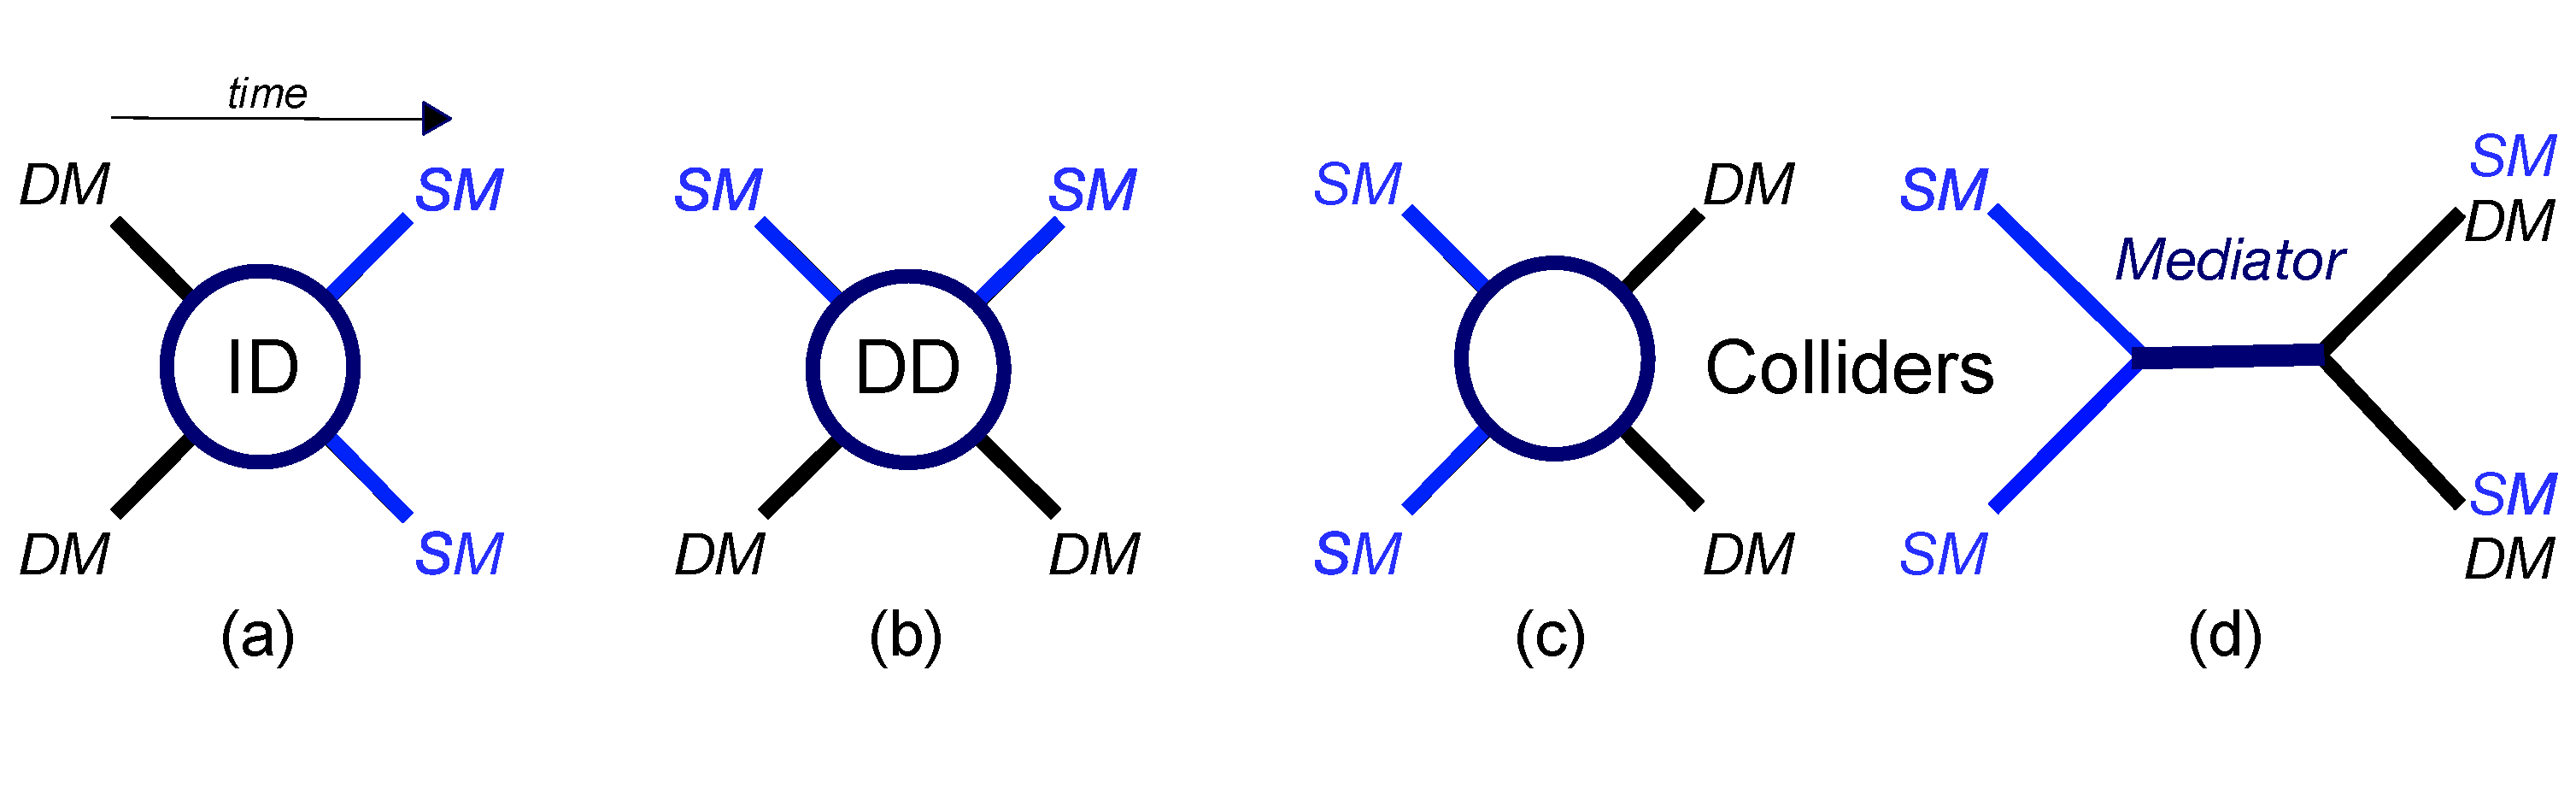
\includegraphics[width=\textwidth]{figures/EFTSimplifiedModels}
\caption{Schematic illustration of Dark Matter interactions and their corresponding experimental detection techniques, with time flowing from left to right. Fig. (a) shows DM annihilation to Standard Model particles, as sought by Indirect Detection (ID) experiments. Fig. (b) shows DM -> SM particle scattering, targeted by Direct Detection (DD) experiments. Fig. (c) shows the production of DM particles from the annihilation of SM particles at colliders. Fig. (d) shows again the pair production of DM at colliders as in (c), but in this case the interaction occurs through a mediator particle between DM and SM particles. From~\cite{monoXfig}, inspired by ~\cite{Bauer:2013ihz}.}
\label{fig:Complementarity}
\end{figure}

It is also worth mentioning that, even though comparisons between collider, DD and ID are becoming the standard for these communities,
the comparison with LHC, DD and ID results with results from astrophysics beyond the relic density is a growing field. 
This is particularly important since all the observational evidence of DM that we have is gravitational,
so DM properties such as mass and density in our and other galaxies
can be inferred from galaxy simulations or deviations in astrophysical observables, 
and signatures of DM self-interactions in rotation galaxies or cluster collisions can complement and verify any DD 
observations. Even though we do not cover this topic in detail in this review we refer to~\cite{Buckley:2017ijx}. 

\subsection{Comparing LHC constraints from visible and invisible searches with non-collider results}

The comparison of results from complementary experiments needs a mechanism to relate the processes
that will produce a signal in each type of detectors. This ultimately means that any comparison between LHC, DD and ID
needs a fully specified theoretical benchmark to be predictive and consistent. Since there are a large possible number of options to choose from, it is always important to keep in mind that such comparisons are model-dependent and the choice of benchmark can have severe implications for the conclusions drawn. 

%%LHC -> DD/ID

%EFT
Tevatron and Run-1 LHC searches mainly used EFTs as the common theoretical ground to compare their constraints on DM across experiments, or full models such as SUSY. EFTs are a good and flexible benchmark model to represent DM interactions in DD and ID experiment, since the momentum transfer of the collision is sufficiently low not to resolve the theory beyond the scale of the interaction and certainly below the electroweak scale. As discussed in Sec.~\ref{sub:EFT}, this is not always the case for high-energy collider experiments. The difference in interaction scales also requires that any operator in the model is evolved from the scale of the LHC collisions to the nuclear scale of DD through renormalization group expansion (RGE)~\cite{DEramo:2014nmf} for full consistency of the results. %is it clear enough that this has to be done for simplified models too? 
An example of a comparison plot between collider and DD results using EFT operators in the WIMP-nucleon cross-section vs WIMP mass plane\footnote{The formulas to translate LHC limits to this plane can be found in Ref.~\cite{Goodman:2010ku}}, without evolving the operators using RGE but showing the effects of the truncation of the events where the EFT is invalid, is shown for the LHC Run-1 results in Fig.~\ref{fig:SIATLASEFT}. %There isn't enough space to describe the results of the truncation in detail
What can be inferred from the plot is that within this class of models and spin assumption %We could have a footnote on SD and SI but no room in text?
the ideal region for the discovery of DM is that where WIMPs have masses above 10 GeV, as both collider and DD experiments are sensitive and could verify each other's claims. Next-generation DD experiments are expected to lower the minimum sensitivity thresholds in the next decade, see e.g.~\cite{Agnese:2016cpb}. 

\begin{figure}[!htpb]
%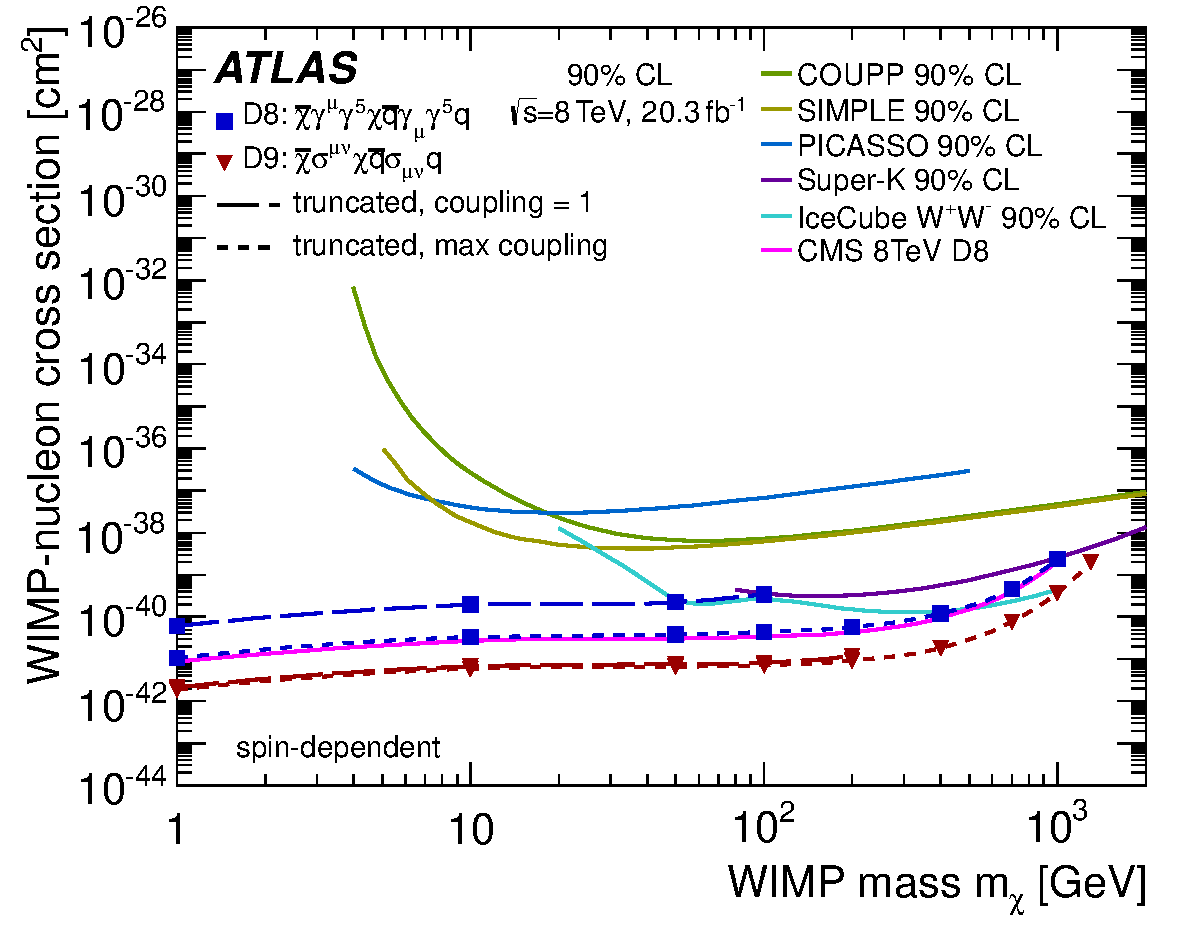
\includegraphics[width=0.35\textwidth]{figures/Monojet8TeV_EFT_SD}
%Can't have both so choose less controversial
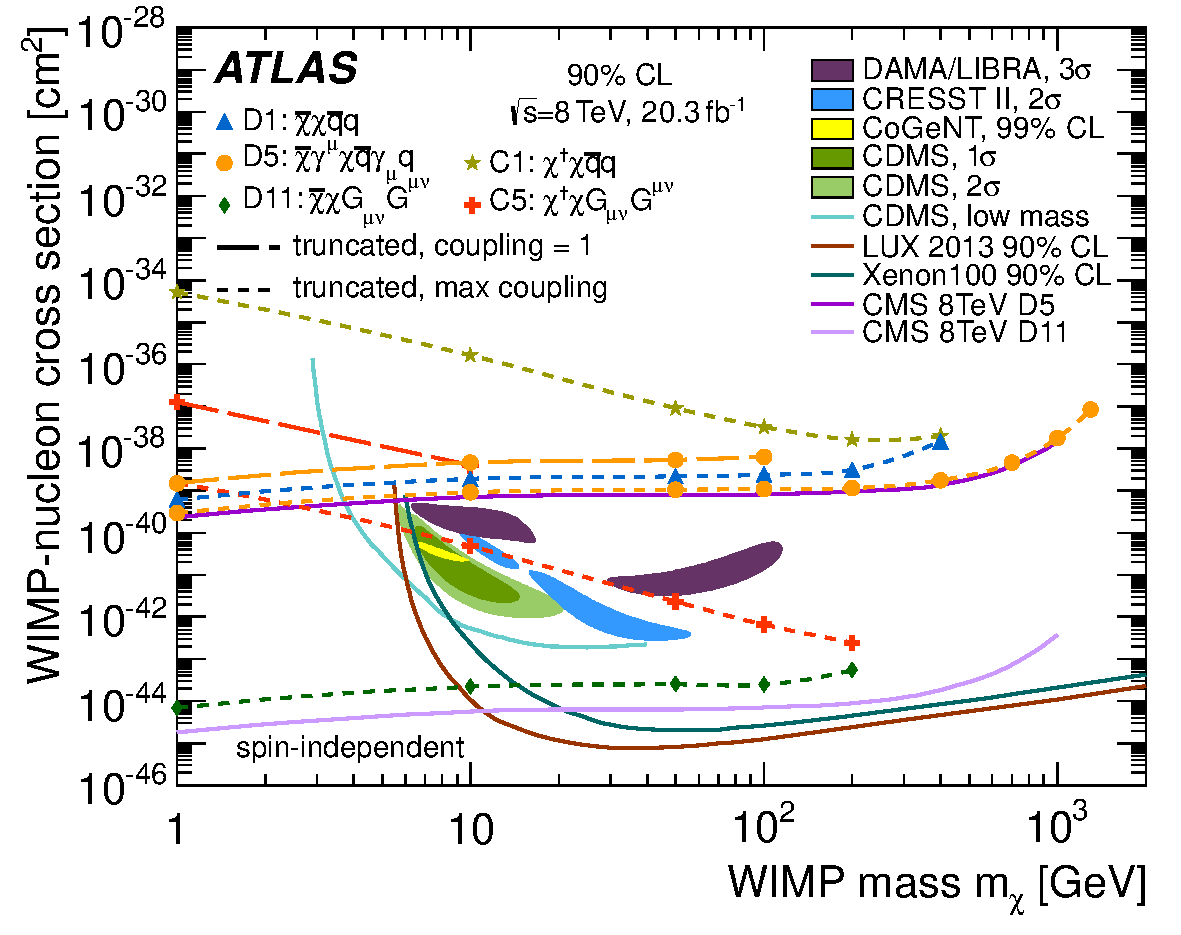
\includegraphics[width=0.9\textwidth]{figures/Monojet8TeV_EFT_SI}
\caption{Inferred 90\% CL limits on (left) the spin-independent and (right) spin-dependent WIMP--nucleon scattering cross section as a function of DM mass m? for different operators. Results from direct-detection experiments for the spin-independent and spin-dependent cross section, and the CMS (untruncated) results are shown for comparison. From~\cite{monoXfig}.}
\label{fig:SIATLASEFT}
\end{figure}

%Simp

\begin{figure}[!htpb]
%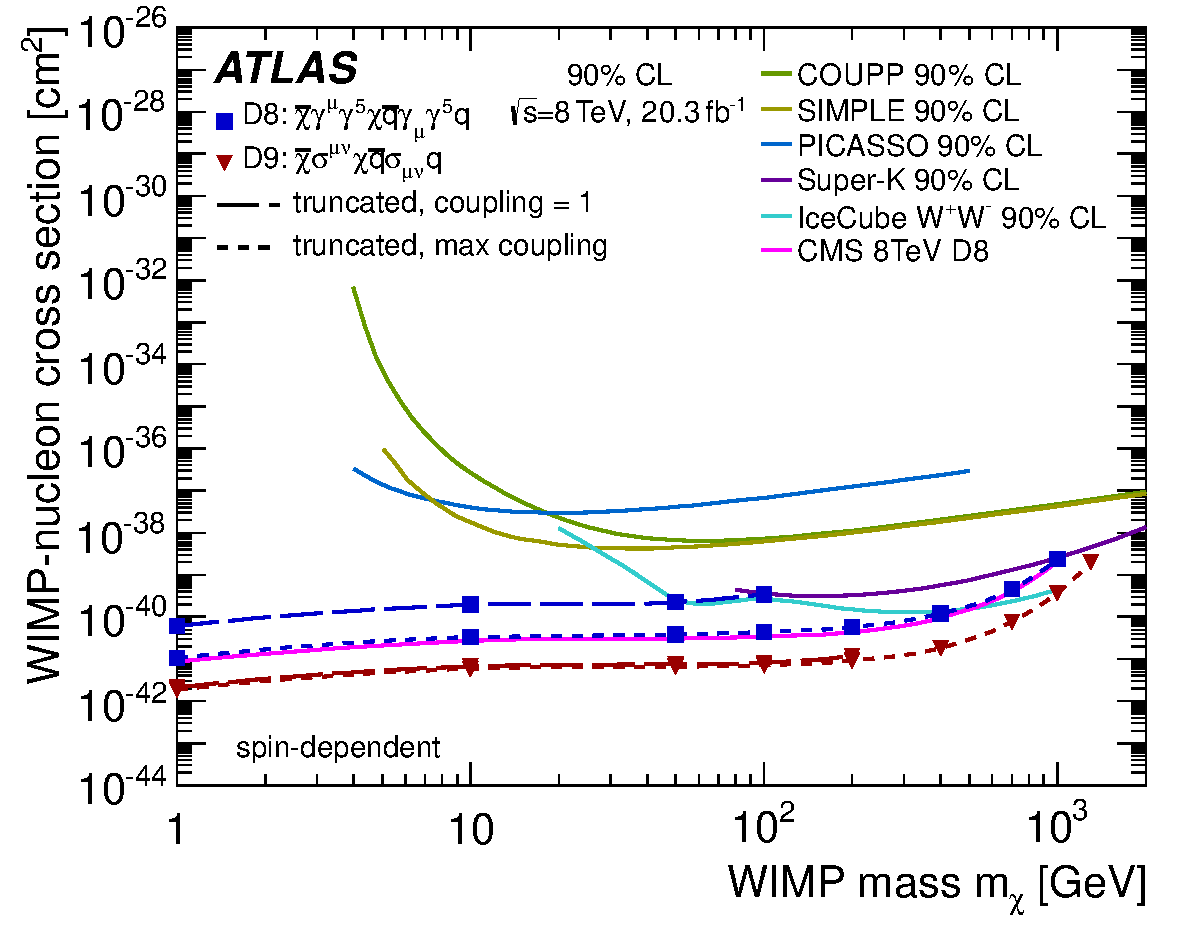
\includegraphics[width=0.35\textwidth]{figures/Monojet8TeV_EFT_SD}
%Can't have both so choose less controversial
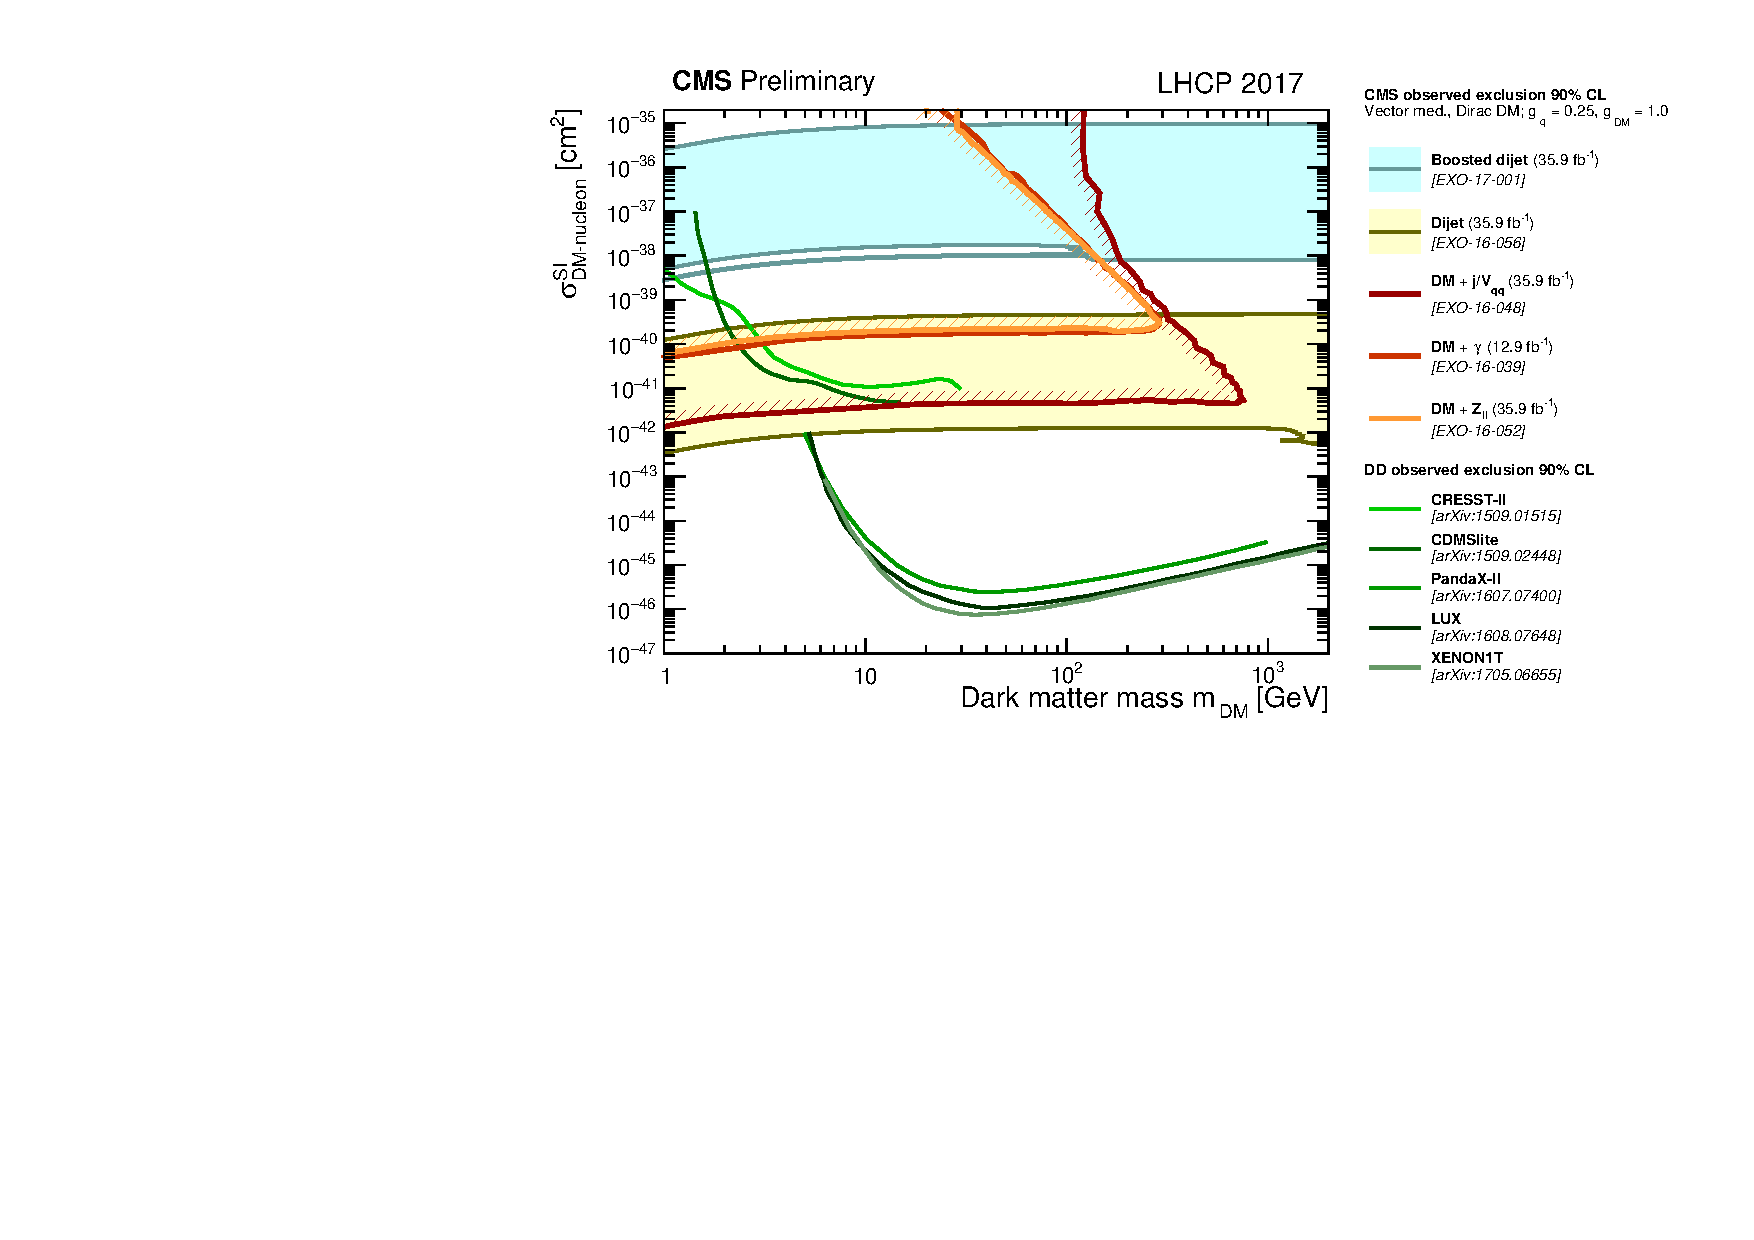
\includegraphics[width=0.9\textwidth]{figures/SI_CMSDD_Summary}
\caption{The 90\% CL CMS constraints in the \mdm-spin-independent DM-nucleon plane, for a vector mediator, Dirac DM and couplings gq = 0.25 and gDM = 1.0, compared with DD experiments. From~\cite{CMSSummary}.}
%We can update if something else comes out
\label{fig:SICMS}
\end{figure}
%Q: use SD? it will piss off more people but maybe we could make that point as well
%We could cite PDG review on spin-dependent vs spin-independent

With the adoption of simplified models of DM by LHC searches in Run-2~\cite{Abercrombie:2015wmb}, the
constraints and caveats of the comparisons between DD and ID have been made clearer, even though the comparisons themselves have become more model-specific and so far privileged vector and axial vector $s-$channel models with fixed coupling values. ATLAS and CMS follow a series of recommendations and well-defined procedure by the Dark Matter Working Group~\cite{Boveia:2016mrp}. LHC experimentalists and theorists have chosen to translate the collider results on visible mediator and invisible DM searches from the \mdm, \mmed plane to the DD and ID planes, so that all information on the results that are reinterpreted are available and all assumptions can be clearly spelled out. An example of such a comparison including the most recent LHC and DD results is shown in Fig.~\ref{fig:SICMSEFT}. In this kind of comparisons, it should be noted that the colliders limits do not include any constraint on the relic density, and that absolute exclusion of the different collider searches as well as their relative importance depend strongly on the benchmark scenario and its coupling. We also note that neither this procedure nor the benchmark models used are explicitly accounting for effects that may be important for mediators with masses below 100 GeV, such as interference and mixing with the X boson, quarkonia resonances and unitarity violation. 
%Could cite this for more consistent w/completion and ID: Jacques:2016dqz, but not sure what it adds, I prefer to talk about Linda's result
For reinterpretation of LHC results and their comparisons to DD and ID for scalar and pseudoscalar mediators, also in the context of 2HDM, see e.g.~\cite{Athron:2017kgt,Banerjee:2017wxi,Ipek:2014gua,Bell:2016ekl}.
%Proposals exist so that the plots should be truncated for cross-sections corresponding to a minimum mass.  
%Q: mention discussion from Landsberg? Would be nice. 
%https://indico.cern.ch/event/563066/contributions/2306614/attachments/1340042/2017991/DMWG-09-20-16.pdf
%Mention how low can one go in mdm - AB knows better here? 
%%DD/ID -> LHC
The comparison of collider and ID results using simplified model benchmarks has received new attention since the publication of~\cite{Boveia:2016mrp}. In traditional comparisons, only one DM annihilation state at a time has been used for the comparison of collider and ID results (e.g. $b\bar{b}$, see for example~\cite{Agrawal:2014una}). The work in~\cite{Carpenter:2016thc} considers multiple final state fermions and interprets ID and LHC results in simplified models with $s-$ and $t-$channel mediators. 

Recently, LHC results have also started to be utilized by DD collaboration for constraints of simplified models of DM, see e.g.\cite{PhysRevLett.118.251301,Balazs:2017hxh}. IceCube and other experiments have used constraints from a MSSM scan, see e.g.~\cite{Aartsen:2016zhm}. The pMSSM is also a good framework to highlight the complementarity of LHC, direct and indirect detection experiments, as shown in e.g. Ref,~\cite{Cahill-Rowley:2014twa}.  %CD: maybe add some quantitative results?

%Would be nice to have a figure but probably too complicated to get as it's published

%Mention Gambit? I would rather describe it in the "SUSY fits" part

%We aren't talking about uncertainties on DD and ID, maybe we should or at least we should cite?
%https://arxiv.org/abs/1409.5446

All experimental results, be it from DD, ID or collider, are affected by experimental and theoretical uncertainties.
%"We advocate that": not sure i want to put that in
A further step towards a more informative comparison between these results is to convey 
an idea of the impact of those uncertainties in the plots. 
The main uncertainties for LHC searches have been outlined in Sec.~\ref{03_ExperimentalResults},
and they are traditionally displayed as one-sigma bands around the LHC constraints. 
Additional uncertainties in the procedure that translate collider results in the DD and ID planes
stem from the matrix elements of the nuclei, but this is an uncertainty that
affects DD as well. %Could make this clearer and cite? 
The situation is less straightforward when comparing collider results to measurements subject to astrophysical
uncertainties (for a summary of DD and ID uncertainties, see~\cite{Feldstein:2014ufa,d300ef23986a49099715e661295a4d72}
and references therein) as those are difficult to estimate and can have a large impact that affects 
different kinds of experiments differently. 
The experimental and theoretical communities have not yet agreed on a common presentation of experimental uncertainties, 
but we expect the discussion will continue in the future. 

\subsection{Comparing LHC constraints from visible and invisible searches with the DM relic density}

%need to match this with the stuff in the introduction and make sure it does not repeat
The observed abundance of DM in the universe today, derived from fits of the Cosmic Microwave Background
measured with the Planck satellite~\cite{Ade:2015xua}, is one
of the few %the only? 
available quantitative DM observations. 
As shown in Fig.~\ref{fig:sensitivityComparison} LHC experiments overlay a line corresponding to 
a dark matter density of $\omega_c = 0.12 h^2$ according to the standard thermal history as calculated
from programs such as MadDM and MicrOMEGas~\cite{Backovic:2015cra,Barducci:2016pcb}, to 
illustrate where a given simplified model is sufficient to explain the observed DM abundance. 

Conclusions on whether a model is ruled out by information on relic density alone cannot be drawn for simplified models, 
as there may be additional physics processes beyond those included in the simplified model that influence the DM abundance.
Moreover, the assumption of a standard thermal history where the current DM density is achieved via freeze-out  
%does the reader know what a standard thermal history is?
%how do we treat the assumption of LambdaCDM? way too big a discussion to start here
is only one of the possibilities~\cite{Bernal:2017kxu}. 
Nevertheless, the relic density remains a useful guiding principle for DM searches if these assumptions are correct~\cite{Busoni:2014gta,Catena:2017xqq}. 

%Confronting the entire set of collider results with the relic density using a full model requires a 
%careful framework that is able to test model points against data. A variety of tools are available for this purpose,
%notably Mastercode~/cite{MC} and Gambit~/cite{G}. [Do we want to describe? Sentence is empty this way but we have no more space]. 

%DMWG 
%Relic density calculations can be overlaid on the mass-mass plot to indicate where the particles and interactions of a specific simplified model are by themselves su cient for explaining the observed DM abundance. For the simplified models recommended by the ATLAS/CMS DM Forum, this curve corresponds to the parameters for which the observed relic abundance is compatible with a single species of DM Dirac fermion and a single mediator that couples to all SM quarks with equal strength. One should not conclude that a simplified model is ruled out for values of model parameters that are inconsistent with the relic density overlay. Rather, one should conclude that additional physics beyond the simplified model was relevant for determining the DM abundance in the early Universe.




\section{FUTURE EVOLUTION OF COLLIDER SEARCHES}
\label{sec:05_Future}
In this chapter, we identify a set of future directions for searches of dark matter at colliders that will become interesting in the coming years. 
We note in any case that this is not an exhaustive list, and gives only a personal perspective. 

Idea here: have a couple of sentences in future directions divided by chapter. One page max. 

%Higgs and Z portals
%For future: mention future e+e- colliders in VH production. 
%New: https://arxiv.org/abs/1712.07237
Mention inclusive vs exclusive searches, monojet is the basic event selection then one selects more things on top of that. 
%Link to:
%Moreover, the sensitivity hierarchy of \MET+X searches does not privilege the jet+\MET final state if there is a direct new physics coupling between a vector boson and the DM, as in the case of the EFT model mentioned in Section~\ref{sub:EFT}, or if the radiated object is a new particle~\cite{Autran:2015mfa}. 
%This latter signal motivates searches in the \MET+generic resonance final state CD: keep for later. 

A generic event selection for excesses of \MET also provides an inclusive sample for more targeted searches as it will be discussed in Chapter~\ref{sec:05_Future}. 

Chapter 2

What models are we developing? 
- the scalar has low x-sec, will be more interesting when we can probe with mu < 1 
- LLPs and why and how
- t-channel are going away from the dominance of s-channel
- SUSY electroweak is the future (Mike Hance's talk?)

%too LLP? "we need this, an example of a way to do it is here"
Motivated by the wide variety of theoretically possible, experimentally challenging long-lived particle signatures, various efforts are ongoing to derive a prioritized set of benchmark models for collider searches in a similar fashion as Ref.~\cite{Abercrombie:2015wmb}. Among the various possibilities, we note the bottom-up approach adopted in~\cite{Buchmueller:2017uqu}, choosing masses and couplings for the models described in~\ref{sub:simplifiedModels} so that they must include a long-lived particle. The categorization of the models by production operator and final state permits to adopt a more systematic set of benchmarks for this kind of signatures. These models can then be mapped onto more complete theories. However, no attempts have yet been made to connect the models in~\cite{Buchmueller:2017uqu} to cosmological history. 

Chapter 3

Remind people of how TLA was developed out of a hole, and in the same way develop simplified model connection to dark photons, are there holes?
- search for other scalars below the Higgs mass, lighter than the Z (1612.07282)
- this will need special triggering strategies, especially track triggers and triggerless readout (cite LHCb's MikeW)

Try and do searches with MET+ISR+weird stuff (or ISR is a new resonance like the Z' but do we really have to cite Whiteson?)

HL-LHC and future colliders a couple of sentences
- phil's stuff: under a particular set of assumptions, only the scalar will be left (i don't like that message)
- making use of highest lumi/CoM requires precise understanding of backgrounds
- some LLP (cite Curtin)

Chapter 4

Next generation of ID and DD, and maybe directional, will give us a lot more results on thermal wimps

%"We advocate that": not sure i want to put that in
A further step towards a more informative comparison between these results is to convey an idea of the impact of those uncertainties in the plots. 
The main uncertainties for LHC searches have been outlined in Sec.~\ref{03_ExperimentalResults}, and they are traditionally displayed as one-sigma bands around the LHC constraints. 
Additional uncertainties in the procedure that translate collider results in the DD and ID planes stem from the matrix elements of the nuclei, but this is an uncertainty that
affects DD as well. %Could make this clearer and cite? 
The situation is less straightforward when comparing collider results to measurements subject to astrophysical uncertainties (for a summary of DD and ID uncertainties, see~\cite{Feldstein:2014ufa,d300ef23986a49099715e661295a4d72} and references therein) as those are difficult to estimate and can have a large impact that affects different kinds of experiments differently. 
The experimental and theoretical communities have not yet agreed on a common presentation of experimental uncertainties, but we expect the discussion will continue in the future. 


It is also worth mentioning that, even though comparisons between collider, DD and ID are becoming the standard for these communities,
the comparison with LHC, DD and ID results with results from astrophysics beyond the relic density is a growing field. 
This is particularly important since all the observational evidence of DM that we have is gravitational,
so DM properties such as mass and density in our and other galaxies
can be inferred from galaxy simulations or deviations in astrophysical observables, 
and signatures of DM self-interactions in rotation galaxies or cluster collisions can complement and verify any DD 
observations. Even though we do not cover this topic in detail in this review we refer to~\cite{Buckley:2017ijx}. 



These are exciting times. %I kinda want to finish with this sentence

\clearpage

% Summary Points, one sentence each
\begin{summary}[SUMMARY POINTS]
\begin{enumerate}
\item Summary point Note. These should be full sentences.
\item Summary point 1. Both broad and targeted searches at the LHC are necessary
\item Summary point 2. The LHC is a mediator-producing machine
\item Summary point 3. DM is a good motivation to implement novel techniques 
\item Summary point 4. DM connected people in the DMF and DMWG, LHC community effort, so the reader can get involved or have questions
\item Summary point 5. Complementarity is important to elucidate DM 
\item Summary point 6. Nevertheless, these benchmark models have motivated novel search techniques
to look for low-coupling, low-mass resonances below the TeV scale that would
have otherwise not been explored in early Run-2 data due to experimental difficulties make same point for dark photons
\end{enumerate}
\end{summary}

% Future Issues
\begin{issues}[FUTURE ISSUES]
\begin{enumerate}
\item Summary point Note. These should be full sentences.
\item Future issue 1. HL-LHC and precision searches
\item Future issue 2. Dark sectors and DM particles near the range of the SM are worth looking for, not just high-mass EW scale WIMPs
\item Future issue 3. Look out for community efforts, try to include DD and ID and low-mass experiments 
\end{enumerate}
\end{issues}

%Disclosure
\section*{DISCLOSURE STATEMENT}
The authors are not aware of any affiliations, memberships, funding, or financial holdings that
might be perceived as affecting the objectivity of this review. 

% Acknowledgements
\section*{ACKNOWLEDGMENTS}
We thank Suchita Kulkarni, Valerio Ippolito, Christian Ohm and Frederik Ruehr for the help and advice in preparing this manuscript. 
We also thank Teng Jian Khoo, Ulrich Haisch, for useful discussion.
Add DOE and ERC grant info. 
% References
%
% Margin notes within bibliography
%\section*{LITERATURE\ CITED}
%To download the appropriate bibliography style file, please see \url{http://www.annualreviews.org/page/authors/author-instructions/preparing/latex}. 
%Please see the Style Guide document for instructions on preparing your Literature Cited.
%The citations should be numbered in order of appearance. For example:

\bibliography{AnnRev_Main}
\bibliographystyle{ar-style5}

\end{document}
